%!TEX ROOT = thesis.tex
\chapter{ Evaluation of Findings/ Research Contribution }
\section{Introduction}
This chapter explained about the findings of the project. The results for homogeneous, heterogeneous, and single ANN model are explained in details. It is also explained the limitation and research contribution to the research community.

\section{Results Discussion}

Each currency is appled to the models individually to get the optimal model for that specific currency. The results of exchange rates forecasting models for six currencies such as United State Dollar (USD), British Pound (GBP), Euro (EUR), Swiss Franc (CHF), Australian Dollar (AUD), and Singapore Dollar (SGD) to Malaysian Ringgit (RM)  are explained in each training ratio with two different ensemble models.

\subsection{USD to RM}

USD currency exchange rates data is given as inputs to train with homogeneous, and heterogeneous ensemble models using three different training datasets ratio such as 80\%, 70\%, and 60\%. 

\subsubsection{Homogeneous Model}

The results of the model which applied with 80\% of the dataset as training dataset are shown in table 6.1. Since 10 predictor orders starting from 3 until 10  are being experimented for the homogeneous model, the optimal model for each predictor order, the number of neurons, RMSE, MAE, activation function and fusion function applied are shown in details.
	
% USD Train 80%
\setlength{\tabcolsep}{0.5em} % for the horizontal padding
{\renewcommand{\arraystretch}{1.2}
	\begin{table}[ht]
		
		\begin{tabular}{@{}rrrrrrr@{}}
			\toprule
			\textbf{PO}&\textbf{Neurons}& \textbf{RMSE} & \textbf{MAE} & \textbf{Act\_F} & \textbf{Learn\_Rate}&\textbf{ Fus\_Fuc} \\ 
			\midrule
			 3 & 12 & 0.0247992772 & 0.0180001557 & tanh & 0.1& MAX \\ 
			 4 & 10 & 0.0243007401 & 0.0173911180 & tanh & 0.1& MAX \\ 
			 5 & 9 & 0.0251915153 & 0.0180703980 & tanh & 0.1 & MAX \\ 
			 6 & 12 & 0.0257844240 & 0.0183796312 & tanh & 0.2 & MAX \\ 
			 7 & 5 & 0.0259657339 & 0.0186208974 & tanh & 0.1 & MAX \\ 
			 8 & 16 & 0.0277265519 & 0.0196592407 & tanh & 0.1 & MEAN \\ 
			 9 & 19 & 0.0255866507 & 0.0183451946 & tanh & 0.1 & MEAN \\ 
			10 & 11 & 0.0257735911 & 0.0188042714 & tanh & 0.1 & MAX \\ 
			\hline
		\end{tabular}
		\hspace*{1cm}
		\caption{Results On USD Homogeneous Model Using 80\% Training Ratio }
	\end{table}	

For the 80\% training ratio, the best optimal model  produced 0.0243007401 RMSE value. This result  is a little higher RMSE error rate compared to the current literature result which is 0.02065 RMSE value \cite{chan:2010}. The best optimal model which has lowest RMSE error is the predictor order 4 with 10 neurons in the hidden layer with the MAX fusion function. The applied activation function is hyperbolic tangent function with the learning rate of 0.1.

The following histogram explain the minimum and maximum error produced by the best optimal model. The bins of the histogram is 0.0079. The bins is based on the range of error values occurred in each model.

\begin{figure}[hbt!]\centering
	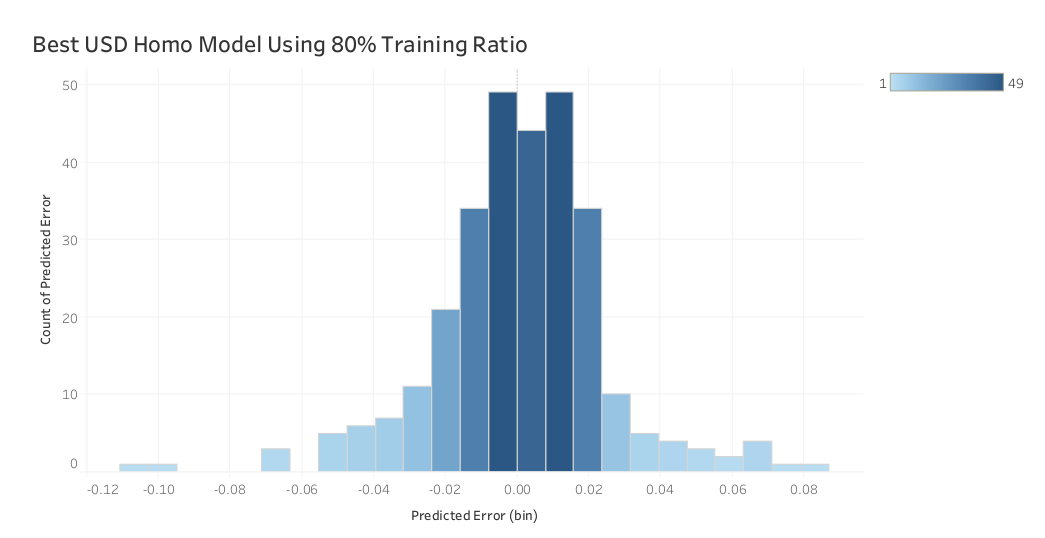
\includegraphics[width=1\textwidth]{homo_usd_80}
	\caption{The error produced by USD Homo model using 80\% training ratio}
\end{figure}
\pagebreak

The testing dataset, 10\% of the datasets, has 295 testing results, therefore 295 errors are produced. Among these errors results, the majority of the errors are in between -0.02 and 0.02. There are some outliers with the values between -0.06 and -0.12. The error, actual and predicted value produced by model are shown in figure 6.2  in graphical manner. The figure 6.2  compared the actual and predicted values in a line graph manner to demonstrate the difference along side with error.


\begin{figure}[hbt!]\centering
	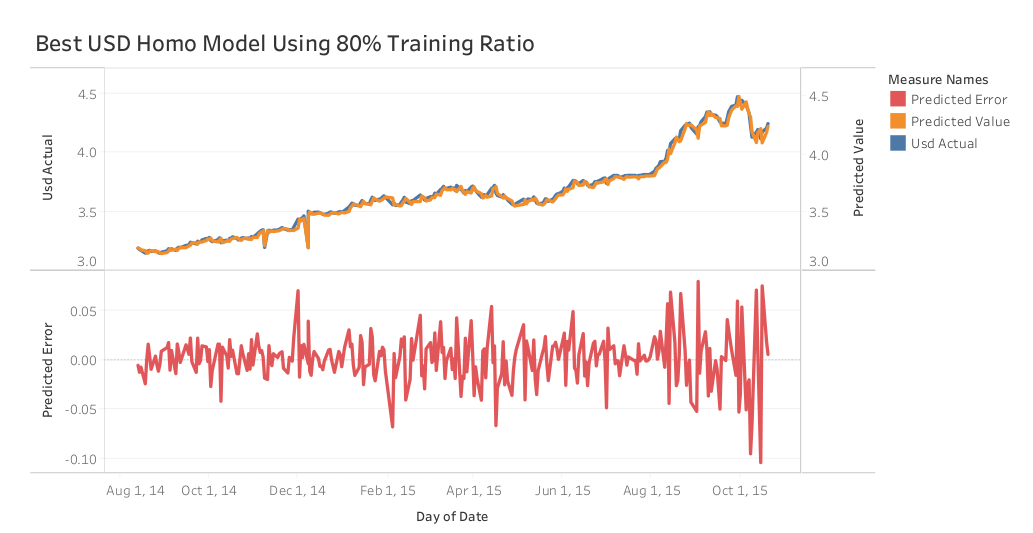
\includegraphics[width=0.9\textwidth]{best_usd_homo_APV_80}
	\caption{The error, actual and predicted produced by USD Homo model  value using 80\% training ratio }
\end{figure}
\pagebreak


The error rate is increased in near December 2014, as well as, in the year end of 2015. Even though it is a bit higher than current literature accuracy , the 80\% of training data ratio can be considered as reliable to some extent. In the figure, it can be seen that most of the error range between -0.05 to 0.05. Some outliers can be spotted in the graph. 

% USD Train 70%

The model which trained with 70\% of the dataset as training dataset are shown in table 6.2. Same like the previous ratio, the model is  experimented with 10 predictor orders for the homogeneous model, the optimal model for each predictor order, the number of neurons, RMSE, MAE, activation function and fusion function applied are shown in details.


The results of the model which trained with 70\% training dataset ratio is shown in following table.

\setlength{\tabcolsep}{0.5em} % for the horizontal padding
{\renewcommand{\arraystretch}{1.2}

\begin{table}[ht]
	\centering
	\begin{tabular}{@{}rrrrrrrr@{}}
		\toprule
		\textbf{PO}&\textbf{Neurons}& \textbf{RMSE} & \textbf{MAE} & \textbf{Act\_F}  & \textbf{Learn\_Rate} &\textbf{ Fus\_Fuc}\\ 
		\midrule
		 3 & 2 & 0.0149640699 & 0.0112025965 & tanh & 0.1 & MAX \\ 
		 4 & 16 & 0.0149954731 & 0.0111664128 & tanh & 0.1 & MAX \\ 
		 5 & 11 & 0.0150098779 & 0.0111655724 & tanh & 0.1 & MAX \\ 
		 6 & 18 & 0.0149943274 & 0.0112014273 & tanh & 0.1 & MAX \\ 
		 7 & 6 & 0.0149067162 & 0.0110502987 & tanh & 0.1 & MAX \\ 
		 8 & 11 & 0.0149265112 & 0.0111363227 & tanh & 0.1 & MAX \\ 
		 9 & 9 & 0.0149356726 & 0.0111709546 & tanh & 0.1 & MAX \\ 
		 10 & 12 & 0.0151702214 & 0.0112393181 & tanh & 0.1& MAX \\ 
		 
		\hline
	\end{tabular}
	\hspace*{1cm}
	\caption{Results On USD Homogeneous Model Using 70\% Training Ratio }
\end{table}

For the model trained with 70\%,  the best optimal model produced 0.0149067162 RMSE value. The result is lower RMSE error rate than the current literature result which is 0.02065 RMSE value \cite{chan:2010}. The best optimal model which has lowest RMSE error is the predictor order 7 with 6 neurons in the hidden layer with the MAX fusion function. The applied activation function hyperbolic tangent function with the learning rate of 0.1.

The histogram below explains the minimum and maximum error produced by the best optimal model. The bandwidth of the histogram is 0.0055.

\begin{figure}[hbt!]\centering
	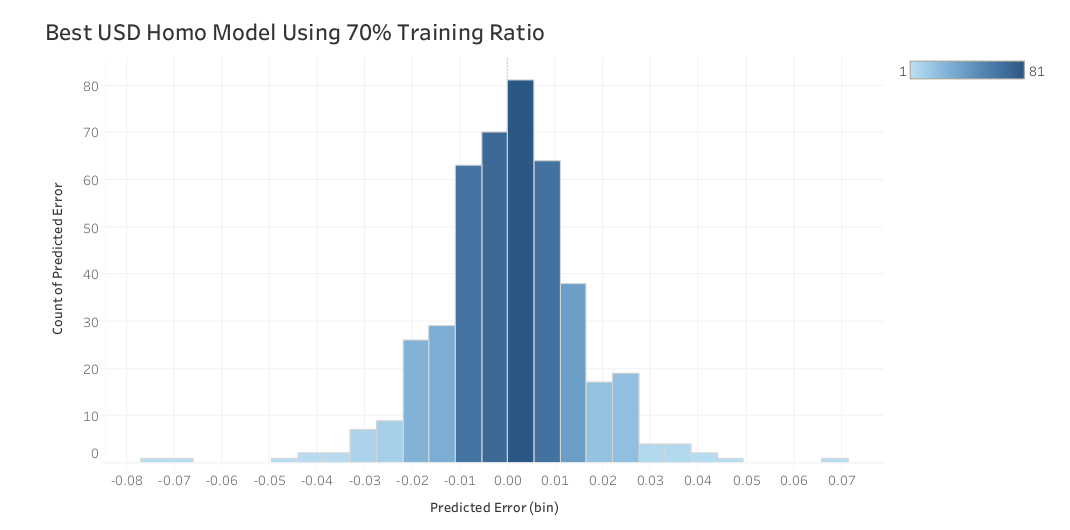
\includegraphics[width=1\textwidth]{homo_usd_70}
	\caption{The error produced by USD Homogeneous model  using 70\% training ratio}
\end{figure}


The testing dataset, 20\% of the datasets, has 443 experiments, which means 443 errors are yield. The majority of errors are range from -0.01 to 0.02. Therefore, this 70\% training ratio produced good reliable accuracy rate compared to 80\% training ratio since majority of the error are in between -0.01 and 0.02.

The error, actual and predicted value produced by model are shown in following figure in graphical manner.  It can said that the error rate is increased in near October 2013, as well as, in the year end of 2014 until 2015. The model from 70\% training ratio yield better than the model from 80\% training ratio.

\begin{figure}[hbt!]\centering
	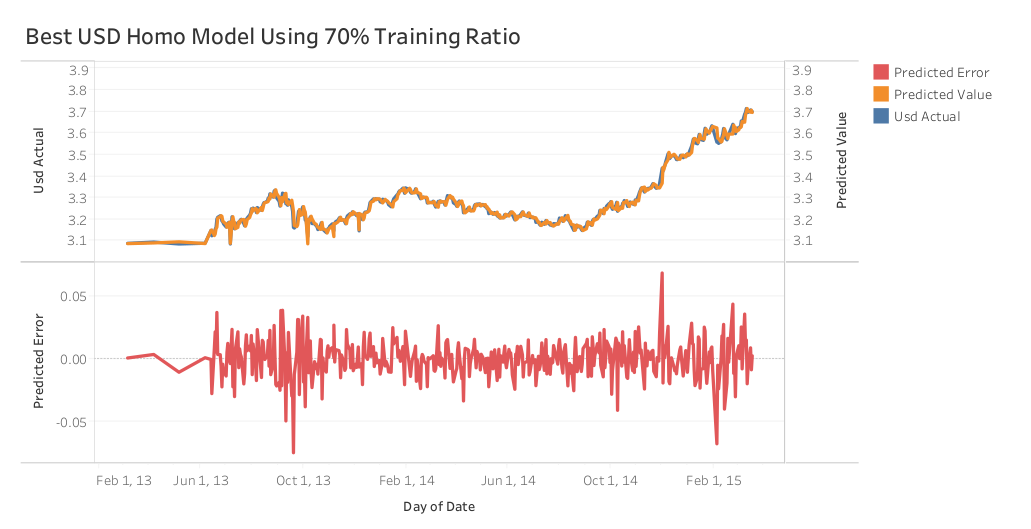
\includegraphics[width=1\textwidth]{best_usd_homo_APV_70}
	\caption{The error, actual and predicted value produced by USD Homo model using 70\% training ratio }
\end{figure}
\pagebreak

 
% USD Train 60% 
The model which trained with 60\% of the dataset as training dataset are shown in the following table. Same like the previous ratio, the model is  experimented with 10 predictor orders for the homogeneous model, the optimal model for each predictor order, the number of neurons, RMSE, MAE, activation function and fusion function applied are shown in details. The results of the model which trained with 60\% training dataset ratio is shown in following table.
\\

\setlength{\tabcolsep}{0.5em} % for the horizontal padding
{\renewcommand{\arraystretch}{1.2}
	
	\begin{table}[ht]
		\centering
		\begin{tabular}{@{}rrrrrrrr@{}}
			\toprule
			\textbf{PO}&\textbf{Neurons}& \textbf{RMSE} & \textbf{MAE} & \textbf{Act\_F}  & \textbf{Learn\_Rate} &\textbf{ Fus\_Fuc}\\ 
			\midrule
			   3 & 8 & 0.0126389229 & 0.0092759801 & tanh & 0.1 & MAX \\ 
			   4 & 6 & 0.0126247514 & 0.0092954307 & tanh & 0.1 & MAX \\ 
			   5 & 11 & 0.0127076343 & 0.0093388155 & tanh & 0.1 & MAX \\ 
			   6 & 13 & 0.0126398482 & 0.0093336256 & tanh & 0.1 & MAX \\ 
			   7 & 17 & 0.0126448159 & 0.0092991726 & tanh & 0.1 & MAX \\ 
			   8 & 16 & 0.0126379473 & 0.0092539342 & tanh & 0.1 & MAX \\ 
			   9 & 9 & 0.0125983879 & 0.0092687522 & tanh & 0.1 & MAX \\ 
			   10 & 16 & 0.0126719687 & 0.0093139147 & tanh & 0.1 & MEAN \\
			\hline
		\end{tabular}
		\hspace*{1cm}
		\caption{Results On USD Homogeneous Model Using 60\% Training Ratio}
	\end{table}
	
For the 60\% training datasets applied model, the best optimal model produced 0.01259839 RMSE value. The result yield highest  accuracy performance  compared to both the previous models and the current literature result. This model is obtained with the predictor order 9 with 9 neurons in the hidden layer with the MAX fusion function. The applied activation function hyperbolic tangent function with the learning rate of 0.1.
	
The histogram below explains the minimum and maximum error produced by the best optimal model. The bandwidth of the histogram is 0.0043.

\begin{figure}[hbt!]\centering
		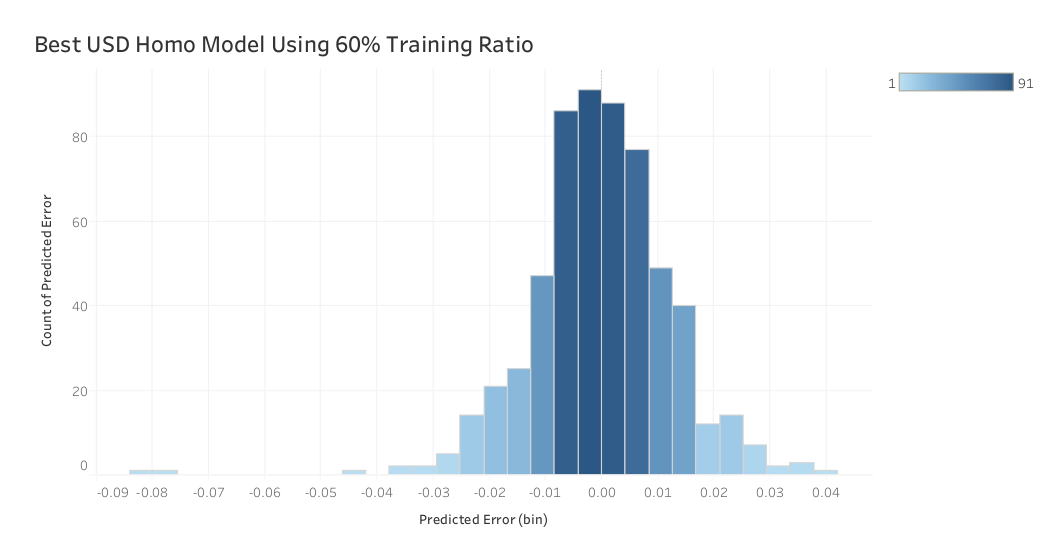
\includegraphics[width=1\textwidth]{homo_usd_60}
		\caption{The error produced by USD Homo model using 60\% training}
\end{figure}
\pagebreak
	
The testing dataset, 20\% of the datasets, has 591 experiments. The most errors are lied between -0.0086 and 0.01. The figure 6.6 compared the actual and predicted values in a line graph manner to demonstrate the difference.It can said that the error rate is increased in near October 2013, as well as, in the year end of 2014 until 2015.\\

\begin{figure}[hbt!]\centering
	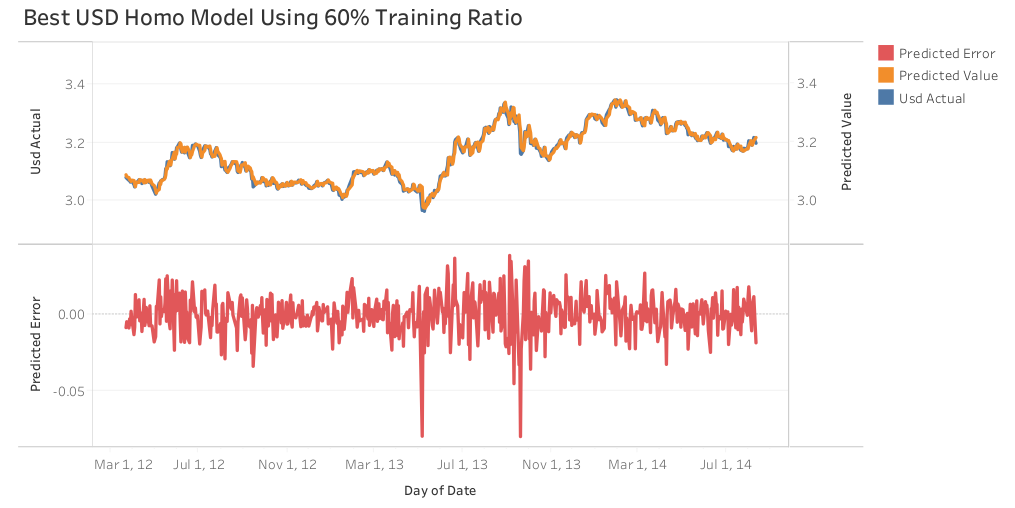
\includegraphics[width=1\textwidth]{best_usd_homo_APV_60}
	\caption{The error, actual and predicted value produced by USD Homo model using 60\% training ratio}
\end{figure}

The table below summarized the outcomes for three training ratio and their best performance of the homogeneous model for USD currency.

\setlength{\tabcolsep}{0.5em} % for the horizontal padding
{\renewcommand{\arraystretch}{1.2}
	
	\begin{table}[ht]
		\centering
		\begin{tabular}{@{}rrrrrrrrr@{}}
			\toprule
		\textbf{Ratio}&\textbf{PO}&\textbf{Neurons}& \textbf{RMSE} & \textbf{MAE} & \textbf{Act\_F} & \textbf{Learn\_Rate} &\textbf{ Fus\_Fuc}\\ 
			\midrule
		60\% & 9 & 9 & 0.012598 & 0.009269 & tanh & 0.1 & MAX \\
		70\% & 7 & 6 & 0.014907 & 0.011050 & tanh & 0.1 & MAX \\ 	
		80\% & 4 & 10 & 0.024301 & 0.017391 & tanh & 0.1& MAX \\
		\hline
	\end{tabular}
	\hspace*{1cm}
	\caption{The three optimal USD Homo models with different training ratio}
	
\end{table}
Among these homogeneous models, the model which trained with 60\% ratio is the best model which yield the lowest RMSE error rate. The second best optimal model produced is the model which trained with 70\% training datasets ratio. The 80\% training datasets ratio yield the higher RMSE error than compared to other two. Therefore, this 60\% training ratio produced the best reliable accuracy rate compared to both  80\% training ratio  and 70\% training ratio models.

\subsubsection{Heterogeneous Model}

The results of the model which applied to heterogeneous model with 80\% of the dataset as training dataset are shown in table

% USD Train 80%
\setlength{\tabcolsep}{0.5em} % for the horizontal padding
{\renewcommand{\arraystretch}{1.2}
	\begin{table}[ht]
		
		\begin{tabular}{@{}rrrrrrr@{}}
			\toprule
			\textbf{PO}&\textbf{Neurons}& \textbf{RMSE} & \textbf{MAE} & \textbf{Act\_F} & \textbf{Learn\_Rate}&\textbf{ Fus\_Fuc} \\ 
			\midrule
			3 & 4 & 0.031532 & 0.023844 & tanh & 0.1 & MAX \\ 
			4 & 10 & 0.028456 & 0.021538 & tanh & 0.1 & MAX \\ 
			5 & 8 & 0.029833 & 0.020852 & tanh & 0.1 & MEAN \\ 
			6 & 7 & 0.036018 & 0.027498 & tanh & 0.1 & MAX \\ 
			7 & 8 & 0.029543 & 0.020445 & tanh & 0.1 & MAX \\ 
			8 & 20 & 0.027242 & 0.018329 & tanh & 0.1 & MAX \\ 
			9 & 17 & 0.031911 & 0.021349 & tanh & 0.1 & MAX \\ 
			10 & 16 & 0.029723 & 0.020743 & tanh & 0.1 & MAX \\ 
			\hline
		\end{tabular}
		\hspace*{1cm}
		\caption{Results On USD Heterogeneous Model Using 80\% Training Ratio }
	\end{table}	
	
	For the 80\% training ratio, the best optimal model  produced 0.027242 RMSE value. This result  is a little higher RMSE error rate compared to the current literature result which is 0.02065 RMSE value \cite{chan:2010}. The best optimal model which has lowest RMSE error is the predictor order 8 with 20 neurons in the hidden layer with the MAX fusion function. The applied activation function is hyperbolic tangent function with the learning rate of 0.1.
	
	The following histogram explain the minimum and maximum error produced by the best optimal model. The bins of the histogram is 0.0212. The bins is based on the range of error values occurred in each model.
	
	\begin{figure}[hbt!]\centering
		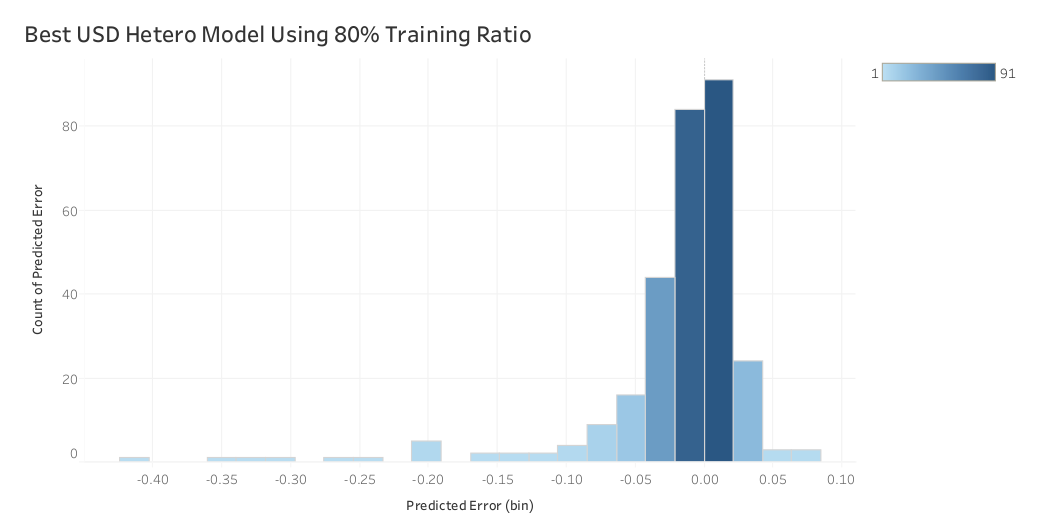
\includegraphics[width=1\textwidth]{hetro_usd_80}
		\caption{The error produced by USD Hetro model using 80\% training ratio}
	\end{figure}
	\pagebreak
	
	The majority of the errors are in between -0.05 and 0.05. The error, actual and predicted value produced by model are shown in figure 6.2  in graphical manner. The following figure compared the actual and predicted values in a line graph manner to demonstrate the difference along side with error.
	
	
	\begin{figure}[hbt!]\centering
		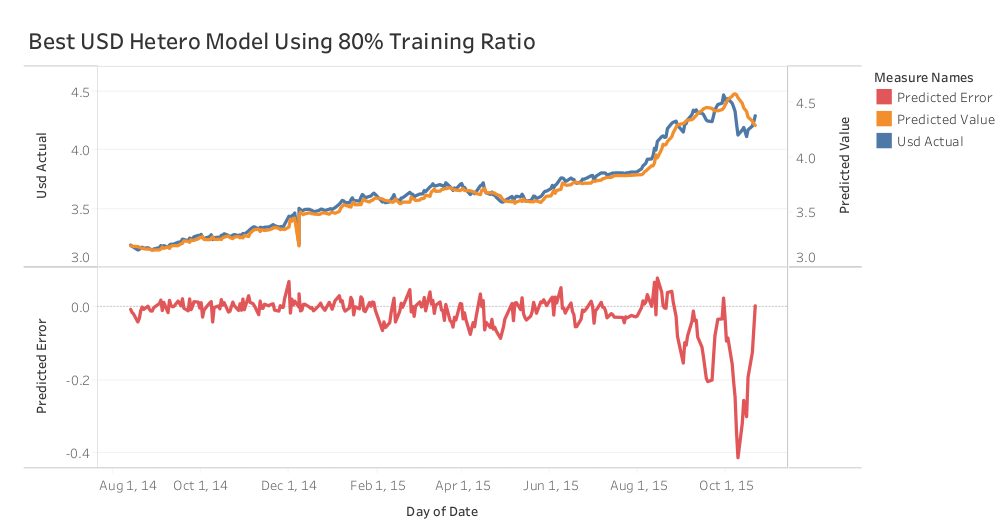
\includegraphics[width=0.9\textwidth]{best_usd_hetero_APV_80}
		\caption{The error, actual and predicted produced by USD Hetero model  value using 80\% training ratio }
	\end{figure}
	\pagebreak
	
	% USD Train 70%
	
	The model which trained with 70\% of the dataset as training dataset are shown in table. Same like the previous ratio, the model is  experimented with 10 predictor orders for the homogeneous model, the optimal model for each predictor order, the number of neurons, RMSE, MAE, activation function and fusion function applied are shown in details.
	
	
	The results of the model which trained with 70\% training dataset ratio is shown in following table.
	
	\setlength{\tabcolsep}{0.5em} % for the horizontal padding
	{\renewcommand{\arraystretch}{1.2}
		
		\begin{table}[ht]
			\centering
			\begin{tabular}{@{}rrrrrrrr@{}}
				\toprule
				\textbf{PO}&\textbf{Neurons}& \textbf{RMSE} & \textbf{MAE} & \textbf{Act\_F}  & \textbf{Learn\_Rate} &\textbf{ Fus\_Fuc}\\ 
				\midrule
				3 & 4 & 0.015116 & 0.011275 & tanh & 0.1 & MAX \\ 
				4 & 14 & 0.015845 & 0.011630 & logistic & 0.1 & MAX \\ 
				5 & 16 & 0.015555 & 0.011540 & tanh & 0.1 & MAX \\ 
				6 & 8 & 0.016041 & 0.011644 & logistic & 0.1 & MAX \\ 
				7 & 9 & 0.016508 & 0.011865 & logistic & 0.1 & MAX \\ 
				8 & 7 & 0.016419 & 0.011802 & logistic & 0.1 & MAX \\ 
				9 & 13 & 0.016889 & 0.012048 & logistic & 0.1 & MAX \\ 
				10 & 16 & 0.015230 & 0.011424 & tanh & 0.1 & MAX \\ 
				
				\hline
			\end{tabular}
			\hspace*{1cm}
			\caption{Results On USD Heterogeneous Model Using 70\% Training Ratio }
		\end{table}
		
		For the model trained with 70\%,  the best optimal model produced 0.015116 RMSE value. The result is lower RMSE error rate than the current literature result which is 0.02065 RMSE value \cite{chan:2010}. The best optimal model which has lowest RMSE error is the predictor order 3 with 4 neurons in the hidden layer with the MAX fusion function. The applied activation function hyperbolic tangent function with the learning rate of 0.1.
		
		The histogram below explains the minimum and maximum error produced by the best optimal model. The bandwidth of the histogram is 0.0055.
		
		\begin{figure}[hbt!]\centering
			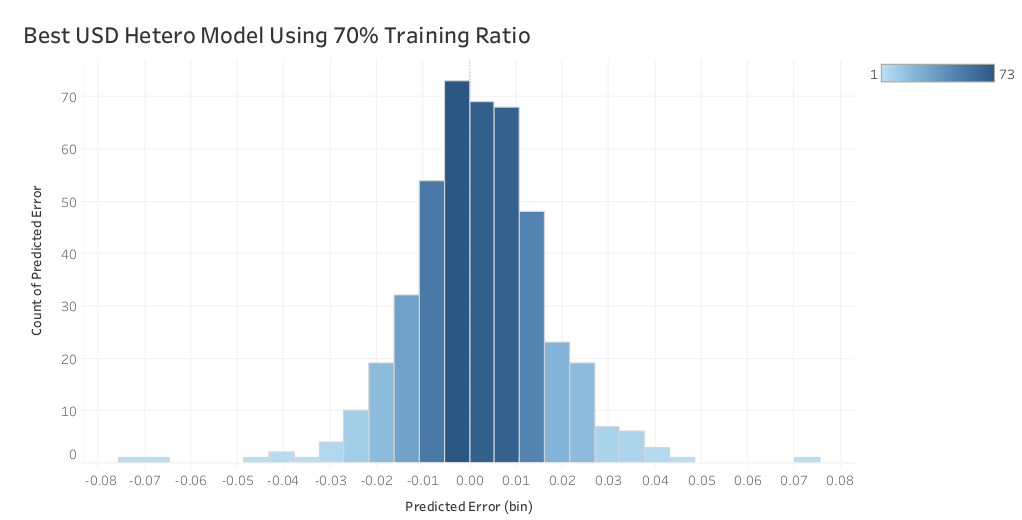
\includegraphics[width=1\textwidth]{hetero_usd_70}
			\caption{The error produced by USD Hetero model  using 70\% training ratio}
		\end{figure}
		\pagebreak
		The majority of errors are range from -0.05 to 0.05. The error, actual and predicted value produced by model are shown in following figure in graphical manner.  
		\begin{figure}[hbt!]\centering
			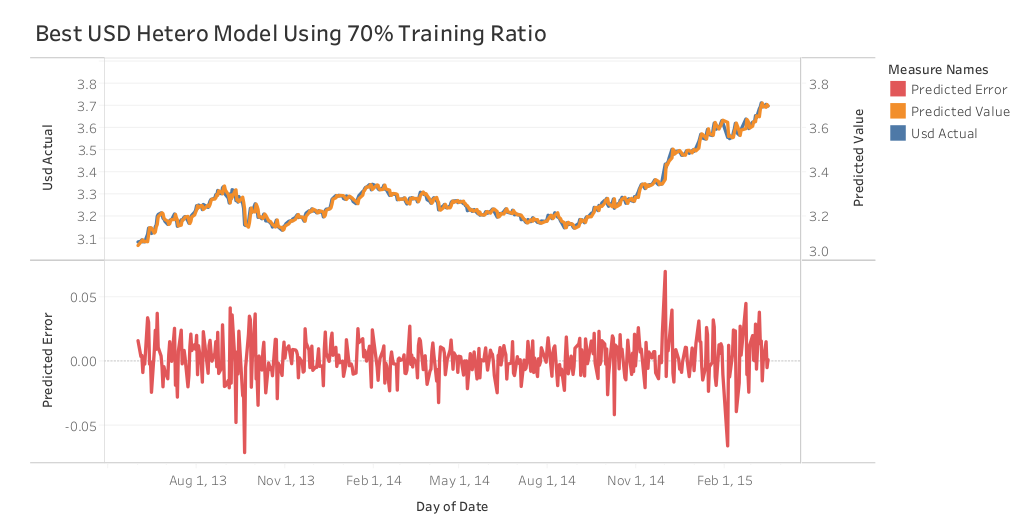
\includegraphics[width=1\textwidth]{best_usd_hetero_APV_70}
			\caption{The error, actual and predicted value produced by USD Hetero model using 70\% training ratio }
		\end{figure}
		\pagebreak
		
		
		% USD Train 60% 
		The model which trained with 60\% of the dataset as training dataset are shown in the following table. Same like the previous ratio, the model is  experimented with 10 predictor orders for the homogeneous model, the optimal model for each predictor order, the number of neurons, RMSE, MAE, activation function and fusion function applied are shown in details. The results of the model which trained with 60\% training dataset ratio is shown in following table.
		\\
		
		\setlength{\tabcolsep}{0.5em} % for the horizontal padding
		{\renewcommand{\arraystretch}{1.2}
			
			\begin{table}[ht]
				\centering
				\begin{tabular}{@{}rrrrrrrr@{}}
					\toprule
					\textbf{PO}&\textbf{Neurons}& \textbf{RMSE} & \textbf{MAE} & \textbf{Act\_F}  & \textbf{Learn\_Rate} &\textbf{ Fus\_Fuc}\\ 
					\midrule
					3 & 17 & 0.012704 & 0.009321 & tanh & 0.1 & MAX \\ 
					4 & 5 & 0.012779 & 0.009452 & tanh & 0.1 & MAX \\ 
					5 & 15 & 0.012739 & 0.009392 & tanh & 0.1 & MAX \\ 
					6 & 7 & 0.012942 & 0.009500 & tanh & 0.1 & MIN \\ 
					7 & 17 & 0.012873 & 0.009463 & tanh & 0.1 & MAX \\ 
					8 & 5 & 0.012788 & 0.009437 & tanh & 0.1 & MAX \\ 
					9 & 15 & 0.012964 & 0.009509 & tanh & 0.1 & MAX \\ 
					10 & 17 & 0.015504 & 0.010932 & logistic & 0.1 & MAX \\ 
					\hline
				\end{tabular}
				\hspace*{1cm}
				\caption{Results On USD Heterogeneous Model Using 60\% Training Ratio}
			\end{table}
			
			For the 60\% training datasets applied model, the best optimal model produced 0.012704 RMSE value. The result yield highest  accuracy performance  compared to both the previous models and the current literature result. This model is obtained with the predictor order 3 with 17 neurons in the hidden layer with the MAX fusion function. The applied activation function hyperbolic tangent function with the learning rate of 0.1.
			
			The histogram below explains the minimum and maximum error produced by the best optimal model. The bandwidth of the histogram is 0.0043.
			
			\begin{figure}[hbt!]\centering
				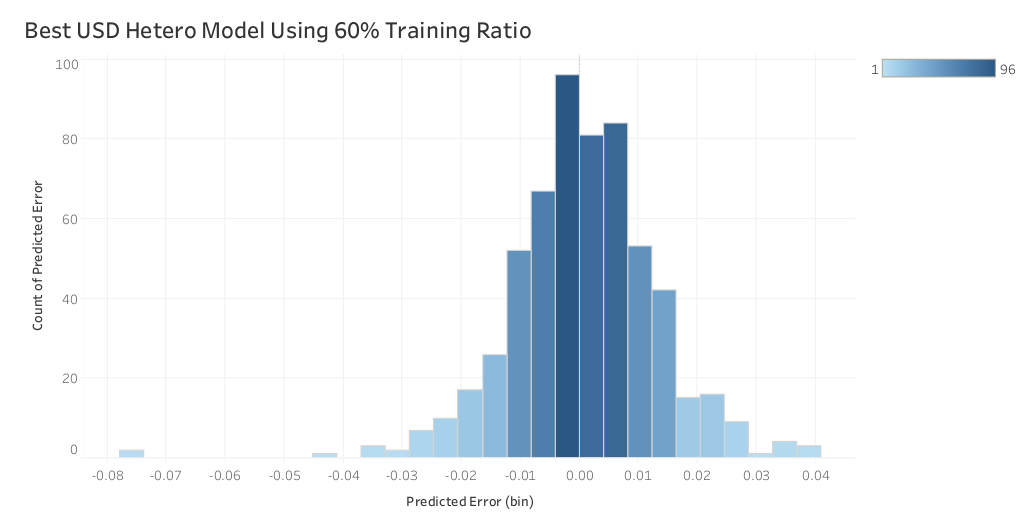
\includegraphics[width=1\textwidth]{hetero_usd_60}
				\caption{The error produced by USD Hetero model using 60\% training}
			\end{figure}
			\pagebreak
			
			The most errors are lied between -0.01 and 0.01. The following figure compared the actual and predicted values in a line graph manner to demonstrate the difference.
			
			\begin{figure}[hbt!]\centering
				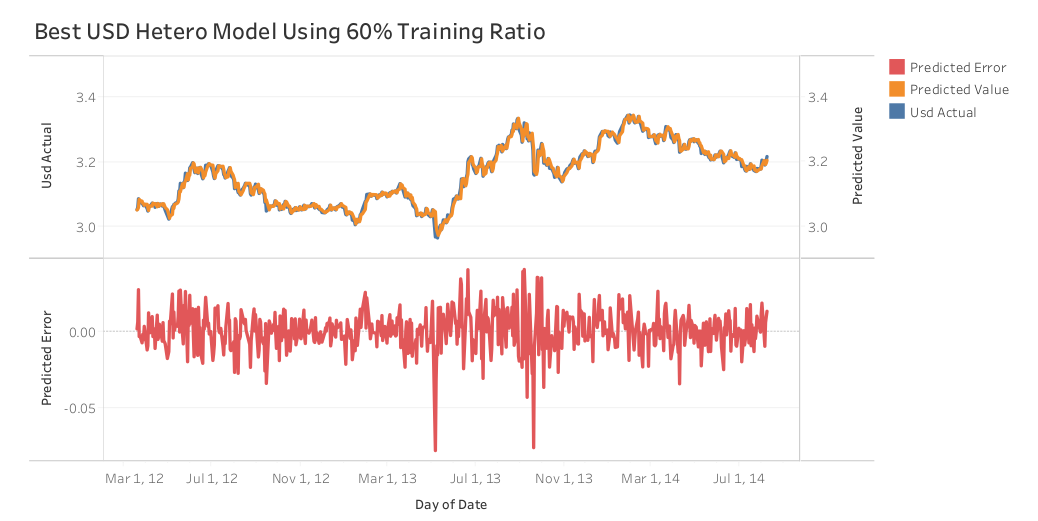
\includegraphics[width=1\textwidth]{best_usd_hetero_APV_60}
				\caption{The error, actual and predicted value produced by USD Hetero model using 60\% training ratio}
			\end{figure}
			
			The table below summarized the outcomes for three training ratio and their best performance of the homogeneous model for USD currency.
			
			\setlength{\tabcolsep}{0.5em} % for the horizontal padding
			{\renewcommand{\arraystretch}{1.2}
				
				\begin{table}[ht]
					\centering
					\begin{tabular}{@{}rrrrrrrrr@{}}
						\toprule
						\textbf{Ratio}&\textbf{PO}&\textbf{Neurons}& \textbf{RMSE} & \textbf{MAE} & \textbf{Act\_F} & \textbf{Learn\_Rate} &\textbf{ Fus\_Fuc}\\ 
						\midrule
						60\% & 3 & 17 & 0.012704 & 0.009321 & tanh & 0.1 & MAX \\
						70\% & 3 & 4 & 0.015116 & 0.011275 & tanh & 0.1 & MAX \\	
						80\% & 8 & 20 & 0.027242 & 0.018329 & tanh & 0.1 & MAX \\
						\hline
					\end{tabular}
					\hspace*{1cm}
					\caption{The three optimal USD Hetero models with different training ratio}
					
				\end{table}
Among these homogeneous models, the model which trained with 60\% ratio is the best model which yield the lowest RMSE error rate. The second best optimal model produced is the model which trained with 70\% training datasets ratio. The 80\% training datasets ratio yield the higher RMSE error than compared to other two. Therefore, this 60\% training ratio produced the best reliable accuracy rate compared to both  80\% training ratio  and 70\% training ratio models.
				
\subsubsection{Ensemble and Single Models}

The optimal two ensemble models for the USD to RM exchange rate are shown together with the training ratio that yield the optimal models and their predictor order, RMSE, MAE, activation function, learning rate, and fusion function applied.
 
\begin{table}[ht]
	\centering
	\begin{tabular}{@{}rrrrrrrrrr@{}}
		\toprule
		\textbf{Ensemble} &\textbf{Ratio}&\textbf{PO}&\textbf{Neurons}& \textbf{RMSE} & \textbf{MAE} & \textbf{Act\_F} & \textbf{LR} &\textbf{ Fus\_Fuc}\\ 
		\midrule
		
		HOMO	& 60\% & 9 & 9 & 0.012598 & 0.009269 & tanh & 0.1 & MAX \\ 	
		HETERO	& 60\% & 3 & 17 & 0.012704 & 0.009321 & tanh & 0.1 & MAX \\
		
		\hline
	\end{tabular}
	\hspace*{1cm}
	\caption{The optimal ensemble  Homo and Hetero models for USD to RM }
	\end{table}
	
Based on the RMSE rate, the homogeneous ensemble model out perform the heterogeneous model. However, the performance accuracy different for both models is not much, and they both yield better accuracy that current literature accuracy rate for the USD to RM exchange.

The three  single models for the USD to RM exchange rate are shown together with the training ratio that yield the optimal models and their predictor order, RMSE, MAE, activation function, and learning rate. Since the homogeneous ensemble yield higher performance accuracy rate, the training parameters from homogeneous model is applied to test in the single models.

\begin{table}[ht]
	\centering
	\begin{tabular}{@{}rrrrrrrrrr@{}}
		\toprule
		\textbf{Single} &\textbf{Ratio}&\textbf{PO}&\textbf{Neurons}& \textbf{RMSE} & \textbf{MAE} & \textbf{Act\_Func} & \textbf{Learn\_Rate} \\ 
		\midrule
		MLP	& 60\% & 9 & 9 & 0.012717 &  0.009399 & tanh & 0.1 \\	
		RNN	& 60\% & 9 & 9 & 0.034810 &  0.026693 & tanh & 0.1 \\
		RBF	& 60\% & 9 & 9 & 0.050619 & 0.045792 & tanh & 0.1  \\
		\hline
	\end{tabular}
	\hspace*{1cm}
	\caption{The optimal three single models for USD to RM }
\end{table}

Among these single network models, only MLP yield the reliable accuracy compared to ensemble networks models. Therefore, the homogeneous ensemble model produce the best optimal accuracy among both ensemble and single models.

	
	

	
% EUR CURRENCY

\subsection{EUR to RM}
EUR currency exchange rates data is given as inputs to train with homogeneous, and heterogeneous ensemble models using three different training datasets ratio such as 80\%, 70\%, and 60\%. 

\subsubsection{Homogeneous Model}

The results of the model which applied with 80\% of the dataset as training dataset are shown in table 6.4. 

% EUR Train 80%
\setlength{\tabcolsep}{0.5em} % for the horizontal padding
{\renewcommand{\arraystretch}{1.2}
	\begin{table}[ht]
		
		\begin{tabular}{@{}rrrrrrr@{}}
			\toprule
			\textbf{PO}&\textbf{Neurons}& \textbf{RMSE} & \textbf{MAE} & \textbf{Act\_F}  & \textbf{Learn\_Rate} &\textbf{ Fus\_Fuc}\\ 
			\midrule
			 3 & 7 & 0.0339226930 & 0.0244421541 & tanh & 0.1 & MAX \\ 
			 4 & 12 & 0.0338502790 & 0.0244173341 & tanh & 0.1 & MAX \\ 
			 5 & 6 & 0.0336998420 & 0.0243903202 & tanh & 0.1& MAX \\ 
			 6 & 11 & 0.0337860187 & 0.0243269493 & tanh & 0.1& MAX \\ 
			 7 & 8 & 0.0337054429 & 0.0245761797 & tanh & 0.1 & MEAN \\ 
			 8 & 14 & 0.0339012770 & 0.0247441538 & logistic & 0.1 & MEAN \\ 
			 9 & 19 & 0.0337353202 & 0.0245331215 & tanh & 0.1& MEAN \\ 
			 10 & 16 & 0.0336048425 & 0.0246993289 & tanh & 0.1 & MAX \\ 
			\hline
		\end{tabular}
		\hspace*{1cm}
		\caption{Results On EUR Homogeneous Model Using 80\% Training Ratio }
	\end{table}	

For the 80\% training ratio, the best optimal model  produced 0.03360484 RMSE value. The best optimal model which has lowest RMSE error is the predictor order 10 with 16 neurons in the hidden layer with the MAX fusion function. The applied activation function is hyperbolic tangent function with the learning rate of 0.1.
	
The following histogram explain the minimum and maximum error produced by the best optimal model. The bins of the histogram is 0.0109. The bins is based on the range of error values occurred in each model.
	
	\begin{figure}[hbt!]\centering
		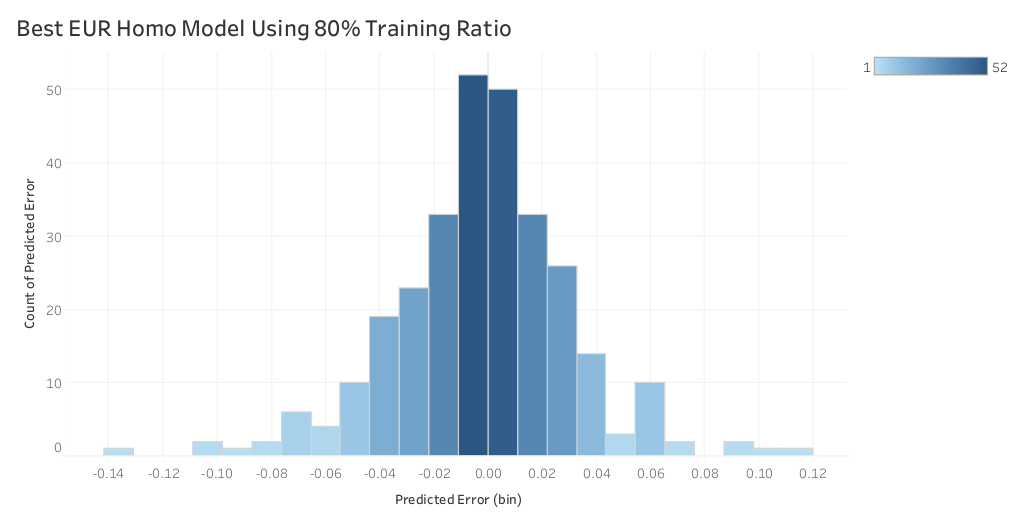
\includegraphics[width=1\textwidth]{homo_eur_80}
		\caption{The error produced by EUR Homo model using 80\% training ratio}
	\end{figure}
	
The testing dataset, 10\% of the datasets, has 295 testing results, therefore 295 errors are produced. Among these errors results, the majority of the errors are in between -0.04 and 0.04. There are some outliers with the values between -0.06 and -0.12. The error, actual and predicted value produced by model are shown in graphical manner. The following figure   compared the actual and predicted values in a line graph manner to demonstrate the difference along side with error.
	
	
	\begin{figure}[hbt!]\centering
		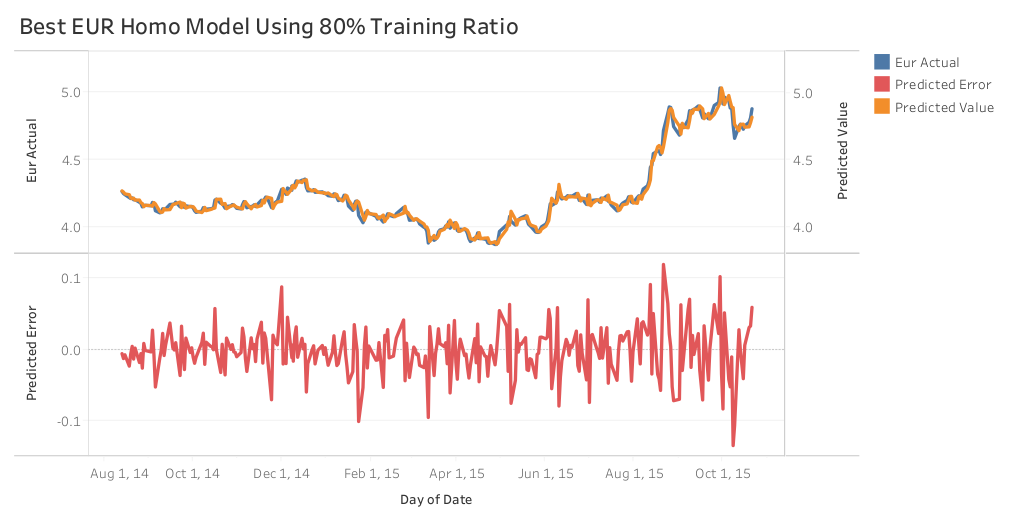
\includegraphics[width=1\textwidth]{best_eur_homo_APV_80}
		\caption{The error, actual and predicted produced by EUR Homo model  value using 80\% training ratio }
	\end{figure}

	
\pagebreak
The error rate is increased in near December 2014 to the year end of 2015.In the figure, it can be seen that most of the error range between -0.1 to 0.1. 

% EUR Train 70%
	
The model which trained with 70\% of the dataset as training dataset are shown in table.

\setlength{\tabcolsep}{0.5em} % for the horizontal padding
{\renewcommand{\arraystretch}{1.2}
		
	\begin{table}[ht]
			\centering
			\begin{tabular}{@{}rrrrrrrr@{}}
				\toprule
				\textbf{PO}&\textbf{Neurons}& \textbf{RMSE} & \textbf{MAE} & \textbf{Act\_F}  & \textbf{Learn\_Rate} &\textbf{ Fus\_Fuc}\\ 
				\midrule
			 3 & 13 & 0.0222215258 & 0.0167280367 & logistic & 0.1 & MAX \\ 
			 4 & 5 & 0.0221860931 & 0.0167081475 & logistic & 0.1 & MAX \\ 
			 5 & 6 & 0.0221670189 & 0.0166938120 & tanh & 0.1 & MAX \\ 
			 6 & 20 & 0.0221118660 & 0.0167119546 & tanh & 0.1 & MAX \\ 
			 7 & 6 & 0.0220479571 & 0.0165676103 & logistic & 0.1 & MAX \\ 
			 8 & 14 & 0.0219801189 & 0.0165407460 & tanh & 0.1 & MAX \\ 
			 9 & 14 & 0.0219828201 & 0.0165368717 & tanh & 0.1 & MAX \\ 
			 10 & 15 & 0.0219806179 & 0.0165080565 & tanh & 0.1& MAX \\ 
			\hline 
				
	\end{tabular}
			\hspace*{1cm}
			\caption{Results On EUR Homogeneous Model Using 70\% Training Ratio }
		\end{table}
		 		
For the model trained with 70\%,  the best optimal model produced 0.02198012 RMSE value. The best optimal model which has lowest RMSE error is the predictor order 8 with 14 neurons in the hidden layer with the MAX fusion function. The applied activation function hyperbolic tangent function with the learning rate of 0.1.
		
The histogram below explains the minimum and maximum error produced by the best optimal model. The bandwidth of the histogram is 0.0072.
		
		\begin{figure}[hbt!]\centering
			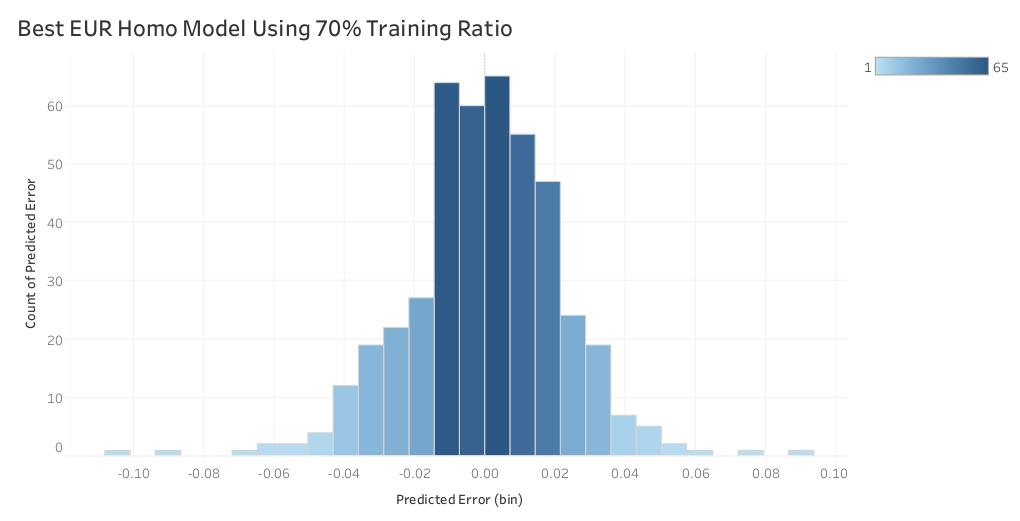
\includegraphics[width=1\textwidth]{homo_eur_70}
			\caption{The error produced by EUR Homogeneous model  using 70\% training ratio}
		\end{figure}
		
		
The testing dataset, 20\% of the datasets, has 443 experiments, which means 443 errors are yield. The majority of errors are range from -0.015 to 0.02. Therefore, this 70\% training ratio produced good reliable accuracy rate compared to 80\% training ratio since majority of the error are in between -0.01 and 0.02.

\begin{figure}[hbt!]\centering
	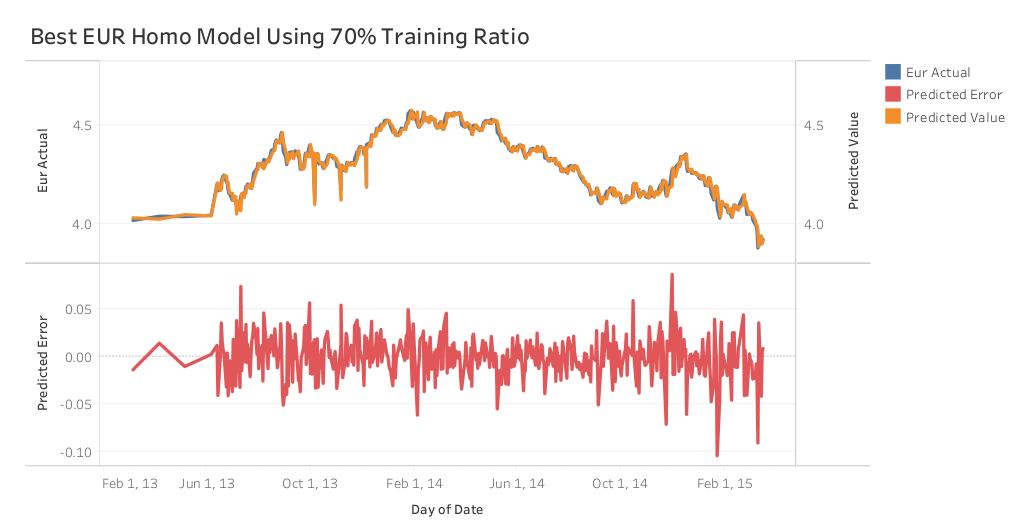
\includegraphics[width=1\textwidth]{best_eur_homo_APV_70}
	\caption{The error, actual and predicted value produced by EUR Homo model using 70\% training ratio }
\end{figure}
\pagebreak

The error, actual and predicted value produced by model are shown in following figure in graphical manner.  It can said that the error rate is increased in staring of year 2015. The model from 70\% training ratio yield better than the model from 80\% training ratio.
		
% EUR Train 60% 
The performance of the model which trained with 60\% of the dataset as training dataset are shown in the following table. 
		
\setlength{\tabcolsep}{0.5em} % for the horizontal padding
{\renewcommand{\arraystretch}{1.2}
	\begin{table}[ht]
				\centering
				\begin{tabular}{@{}rrrrrrrr@{}}
					\toprule
					\textbf{PO}&\textbf{Neurons}& \textbf{RMSE} & \textbf{MAE} & \textbf{Act\_F}  & \textbf{Learn\_Rate}&\textbf{ Fus\_Fuc}\\ 
					\midrule
			 3 & 8 & 0.0191164927 & 0.0146161327 & tanh & 0.1 & MIN \\ 
			 4 & 6 & 0.0191093934 & 0.0146561527 & tanh & 0.1 & MEAN \\ 
			 5 & 7 & 0.0191212515 & 0.0147426950 & tanh & 0.1 & MEAN \\ 
			 6 & 11 & 0.0191805262 & 0.0146793531 & logistic & 0.1 & MEAN \\ 
			 7 & 5 & 0.0191199849 & 0.0146579718 & tanh & 0.1& MIN \\ 
			 8 & 7 & 0.0191491369 & 0.0147424623 & tanh & 0.1 & MEAN \\ 
			9 & 10 & 0.0190938455 & 0.0146765891 & logistic & 0.1 & MIN \\ 
		   10 & 19 & 0.0190871132 & 0.0147453517 & logistic & 0.1 & MIN \\			
			\hline
				\end{tabular}
				\hspace*{1cm}
				\caption{Results On EUR Homogeneous Model Using 60\% Training Ratio}
	\end{table}
			
For the 60\% training datasets applied model, the best optimal model produced 0.0191164927 RMSE value. The result yield highest  accuracy performance  compared to both the previous models and the current literature result. This model is obtained with the predictor order 3 with 8 neurons in the hidden layer with the MIN fusion function. The applied activation function hyperbolic tangent function with the learning rate of 0.1.
			
The histogram below explains the minimum and maximum error produced by the best optimal model. The bandwidth of the histogram is 0.0055.
			
	\begin{figure}[hbt!]\centering
			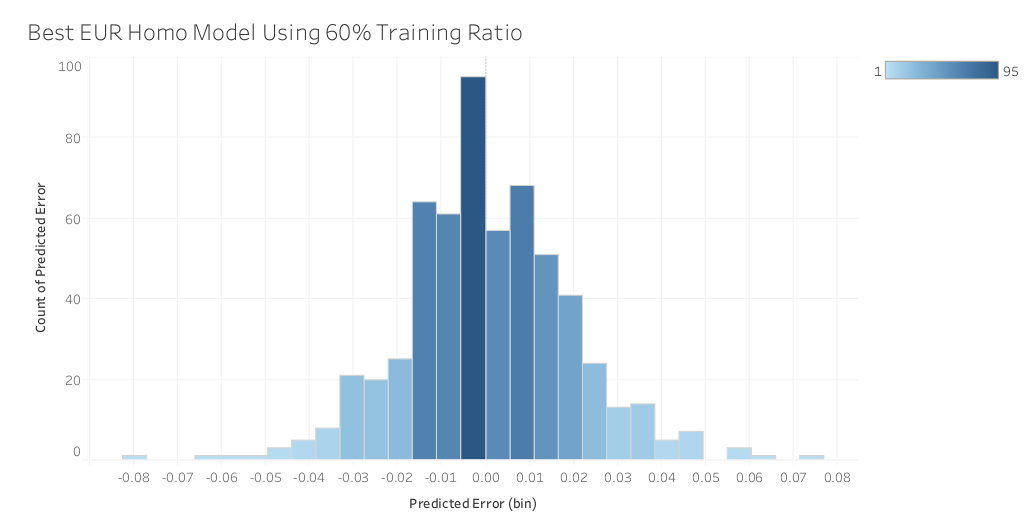
\includegraphics[width=1\textwidth]{homo_eur_60}
			\caption{The error produced by EUR Homo model using 60\%
				training}
	\end{figure}

			
The testing dataset, 20\% of the datasets, has 591 experiments. The most errors are lied between -0.019 and 0.019. The figure below compared the actual and predicted values in a line graph manner to demonstrate the difference.\\
			
	\begin{figure}[hbt!]\centering
		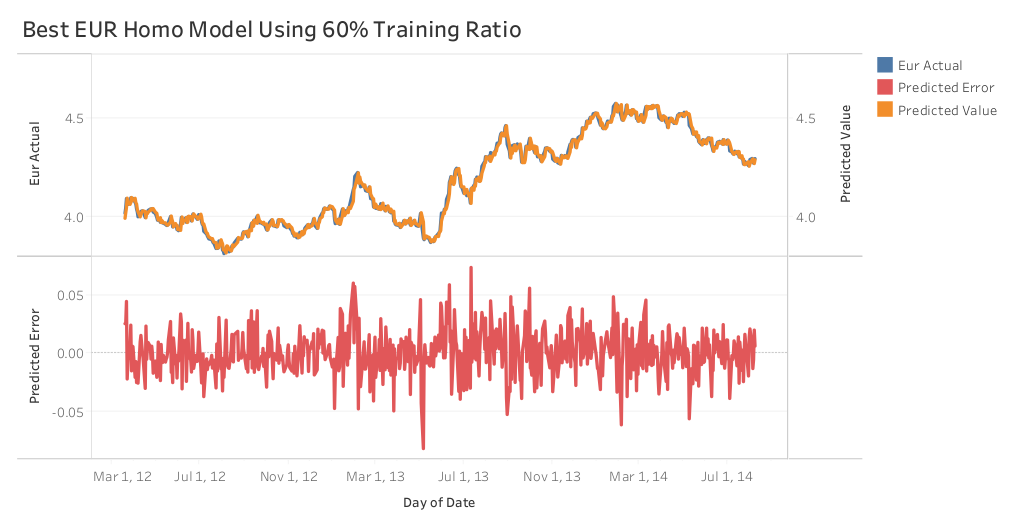
\includegraphics[width=1\textwidth]{best_eur_homo_APV_60}
		\caption{The error, actual and predicted value produced by EUR Homo model using 60\% training ratio}
	\end{figure}
	\pagebreak


The Table 6.8 summarized the outcomes for three training ratio and their best performance of the homogeneous model for EUR currency.

\setlength{\tabcolsep}{0.5em} % for the horizontal padding
{\renewcommand{\arraystretch}{1.2}
	
	\begin{table}[ht]
		\centering
		\begin{tabular}{@{}rrrrrrrrr@{}}
			\toprule
			\textbf{Ratio}&\textbf{PO}&\textbf{Neurons}& \textbf{RMSE} & \textbf{MAE} & \textbf{Act\_F} & \textbf{Learn\_Rate} &\textbf{ Fus\_Fuc}\\ 
			\midrule
			60\% & 3 & 8 & 0.019116 & 0.014616 & tanh & 0.1 & MIN \\ 
			70\% &  8 & 14 & 0.021980 & 0.016541 & tanh & 0.1 & MAX \\	
			80\% & 10 & 16 & 0.033605 & 0.024699 & tanh & 0.1 & MAX \\ 
			\hline
		\end{tabular}
		\hspace*{1cm}
		\caption{The three optimal EUR Homo models with different training ratio}
		
	\end{table}

Among these homogeneous models, the model which trained with 60\% ratio is the best model which yield the lowest RMSE error rate. The second best optimal model produced is the model which trained with 70\% training datasets ratio. The 80\% training datasets ratio yield the higher RMSE error than compared to other two. Therefore, this 60\% training ratio produced the best reliable accuracy rate compared to both  80\% training ratio  and 70\% training ratio models.

\subsubsection{Heterogeneous Model}

The results of the model which applied to heterogeneous model with 80\% of the dataset as training dataset are shown in table

% EUR Train 80%
\setlength{\tabcolsep}{0.5em} % for the horizontal padding
{\renewcommand{\arraystretch}{1.2}
	\begin{table}[ht]
		
		\begin{tabular}{@{}rrrrrrr@{}}
			\toprule
			\textbf{PO}&\textbf{Neurons}& \textbf{RMSE} & \textbf{MAE} & \textbf{Act\_F} & \textbf{Learn\_Rate}&\textbf{ Fus\_Fuc} \\ 
			\midrule
			 3 & 11 & 0.036177 & 0.025778 & logistic & 0.1 & MEAN \\ 
			 4 & 16 & 0.039176 & 0.027597 & logistic & 0.1 & MEAN \\ 
			 5 & 14 & 0.034322 & 0.024755 & tanh & 0.1 & MAX \\ 
			 6 & 19 & 0.039191 & 0.028041 & logistic & 0.1 & MEAN \\ 
			 7 & 20 & 0.038268 & 0.027482 & logistic & 0.1 & MEAN \\ 
			 8 & 15 & 0.034412 & 0.025085 & tanh & 0.1 & MAX \\ 
			 9 & 20 & 0.034823 & 0.025187 & tanh & 0.1 & MAX \\ 
			 10 & 19 & 0.036925 & 0.026207 & logistic & 0.1 & MEAN \\  
			\hline
		\end{tabular}
		\hspace*{1cm}
		\caption{Results On EUR Heterogeneous Model Using 80\% Training Ratio }
	\end{table}	
	
For the 80\% training ratio, the best optimal model  produced 0.034322 RMSE value. The best optimal model which has lowest RMSE error is the predictor order 5 with 14 neurons in the hidden layer with the MAX fusion function. The applied activation function is hyperbolic tangent function with the learning rate of 0.1.
	
The following histogram explain the minimum and maximum error produced by the best optimal model. The bins of the histogram is 0.0144. The bins is based on the range of error values occurred in each model.
	
	\begin{figure}[hbt!]\centering
		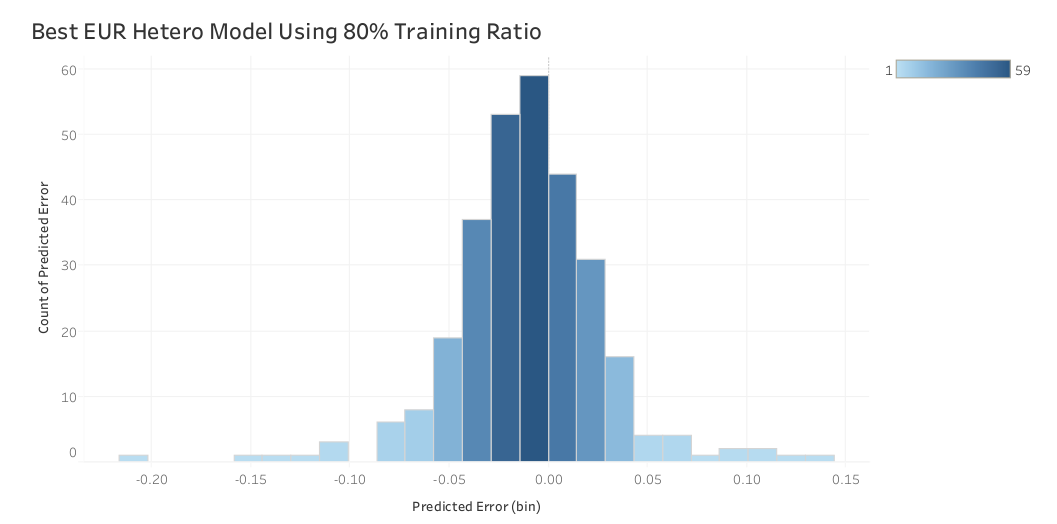
\includegraphics[width=1\textwidth]{hetro_eur_80}
		\caption{The error produced by EUR Hetro model using 80\% training ratio}
	\end{figure}
	\pagebreak
	
The majority of the errors are in between -0.05 and 0.05. The error, actual and predicted value produced by model are shown  in graphical manner. The following figure compared the actual and predicted values in a line graph manner to demonstrate the difference along side with error.
	
	
	\begin{figure}[hbt!]\centering
		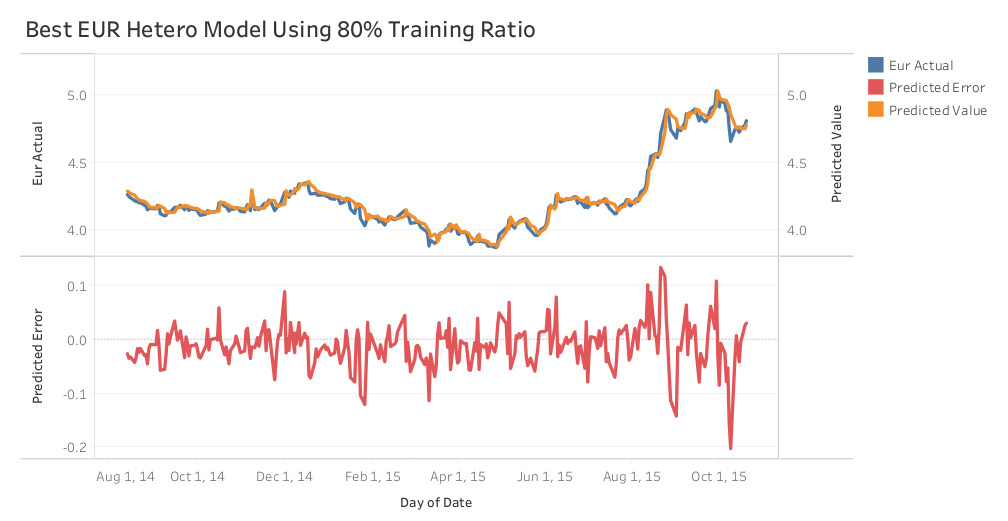
\includegraphics[width=0.9\textwidth]{best_eur_hetero_APV_80}
		\caption{The error, actual and predicted produced by EUR Hetero model  value using 80\% training ratio }
	\end{figure}
	\pagebreak
	
	% EUR Train 70%
	
The model which trained with 70\% of the dataset as training dataset are shown in table. Same like the previous ratio, the model is  experimented with 10 predictor orders for the homogeneous model, the optimal model for each predictor order, the number of neurons, RMSE, MAE, activation function and fusion function applied are shown in details.
	
	
The results of the model which trained with 70\% training dataset ratio is shown in following table.
	
	\setlength{\tabcolsep}{0.5em} % for the horizontal padding
	{\renewcommand{\arraystretch}{1.2}
		
		\begin{table}[ht]
			\centering
			\begin{tabular}{@{}rrrrrrrr@{}}
				\toprule
				\textbf{PO}&\textbf{Neurons}& \textbf{RMSE} & \textbf{MAE} & \textbf{Act\_F}  & \textbf{Learn\_Rate} &\textbf{ Fus\_Fuc}\\ 
				\midrule
				 3 & 6 & 0.022356 & 0.016851 & tanh & 0.1 & MAX \\ 
				 4 & 7 & 0.022340 & 0.016780 & tanh & 0.1 & MIN \\ 
				 5 & 20. & 0.022310 & 0.016887 & tanh & 0.1 & MAX \\ 
				 6 & 15 & 0.022244 & 0.016819 & tanh & 0.1 & MIN \\ 
				 7 & 8 & 0.022086 & 0.016629 & tanh & 0.1 & MIN \\ 
				 8 & 18 & 0.022215 & 0.016770 & tanh & 0.1 & MIN \\ 
				 9 & 16 & 0.024588 & 0.018394 & logistic & 0.1 & MEAN \\ 
				 10 & 6 & 0.022172 & 0.016761 & tanh & 0.1 & MAX \\ 
				\hline
			\end{tabular}
			\hspace*{1cm}
			\caption{Results On EUR Heterogeneous Model Using 70\% Training Ratio }
		\end{table}
		
For the model trained with 70\%,  the best optimal model produced 0.022086 RMSE value. The best optimal model which has lowest RMSE error is the predictor order 7 with 8 neurons in the hidden layer with the MIN fusion function. The applied activation function hyperbolic tangent function with the learning rate of 0.1.
		
The histogram below explains the minimum and maximum error produced by the best optimal model. The bandwidth of the histogram is 0.0055.
		
		\begin{figure}[hbt!]\centering
			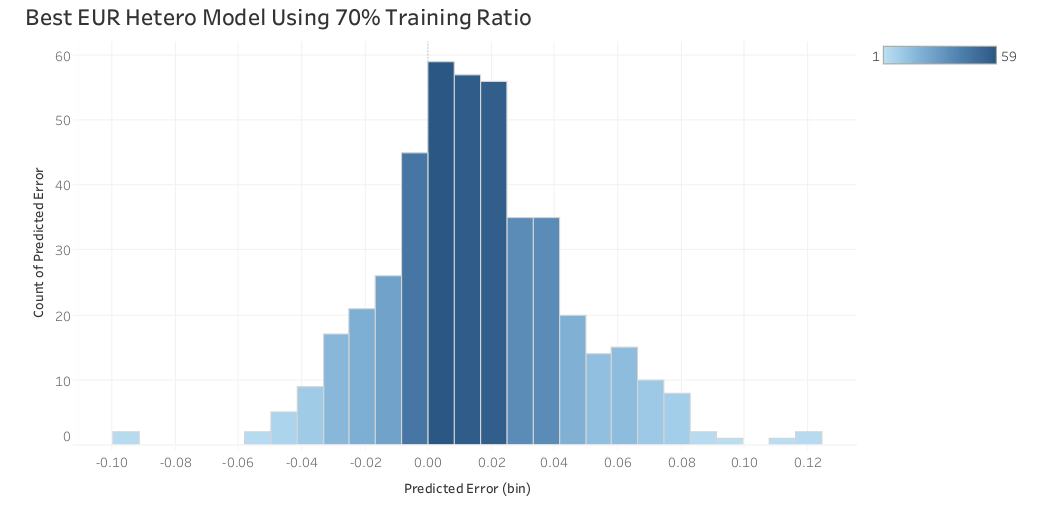
\includegraphics[width=1\textwidth]{hetero_eur_70}
			\caption{The error produced by EUR Hetero model  using 70\% training ratio}
		\end{figure}
		\pagebreak
The majority of errors are range from -0.05 to 0.05. The error, actual and predicted value produced by model are shown in following figure in graphical manner.  
		\begin{figure}[hbt!]\centering
			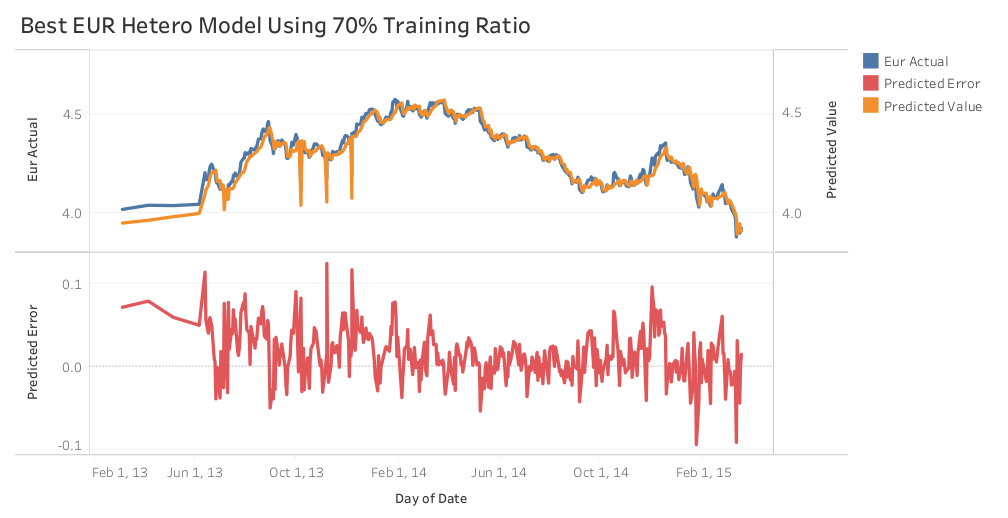
\includegraphics[width=1\textwidth]{best_eur_hetero_APV_70}
			\caption{The error, actual and predicted value produced by EUR Hetero model using 70\% training ratio }
		\end{figure}
		\pagebreak
		
% EUR Train 60% 
The model which trained with 60\% of the dataset as training dataset are shown in the following table. Same like the previous ratio, the model is  experimented with 10 predictor orders for the homogeneous model, the optimal model for each predictor order, the number of neurons, RMSE, MAE, activation function and fusion function applied are shown in details. The results of the model which trained with 60\% training dataset ratio is shown in following table.
		\\
		
		\setlength{\tabcolsep}{0.5em} % for the horizontal padding
		{\renewcommand{\arraystretch}{1.2}
			
			\begin{table}[ht]
				\centering
				\begin{tabular}{@{}rrrrrrrr@{}}
					\toprule
					\textbf{PO}&\textbf{Neurons}& \textbf{RMSE} & \textbf{MAE} & \textbf{Act\_F}  & \textbf{Learn\_Rate} &\textbf{ Fus\_Fuc}\\ 
					\midrule
					 3 & 3 & 0.019668 & 0.015139 & tanh & 0.1 & MAX \\ 
					 4 & 8 & 0.021279 & 0.016299 & tanh & 0.1 & MAX \\ 
					 5 & 15 & 0.023681 & 0.017228 & logistic & 0.1 & MIN \\ 
					 6 & 20 & 0.023745 & 0.017433 & logistic & 0.1 & MIN \\ 
					 7 & 18 & 0.021192 & 0.016901 & tanh & 0.1 & MAX \\ 
					 8 & 13 & 0.025805 & 0.019950 & tanh & 0.1 & MAX \\ 
					 9 & 15 & 0.021746 & 0.016290 & logistic & 0.1 & MIN \\ 
					 10 & 19 & 0.021767 & 0.016251 & logistic & 0.1 & MIN \\ 
					\hline
				\end{tabular}
				\hspace*{1cm}
				\caption{Results On EUR Heterogeneous Model Using 60\% Training Ratio}
			\end{table}
			
For the 60\% training datasets applied model, the best optimal model produced 0.019668 RMSE value.  This model is obtained with the predictor order 3 with 3 neurons in the hidden layer with the MAX fusion function. The applied activation function hyperbolic tangent function with the learning rate of 0.1.
			
The histogram below explains the minimum and maximum error produced by the best optimal model. The bandwidth of the histogram is 0.0045.
			
			\begin{figure}[hbt!]\centering
				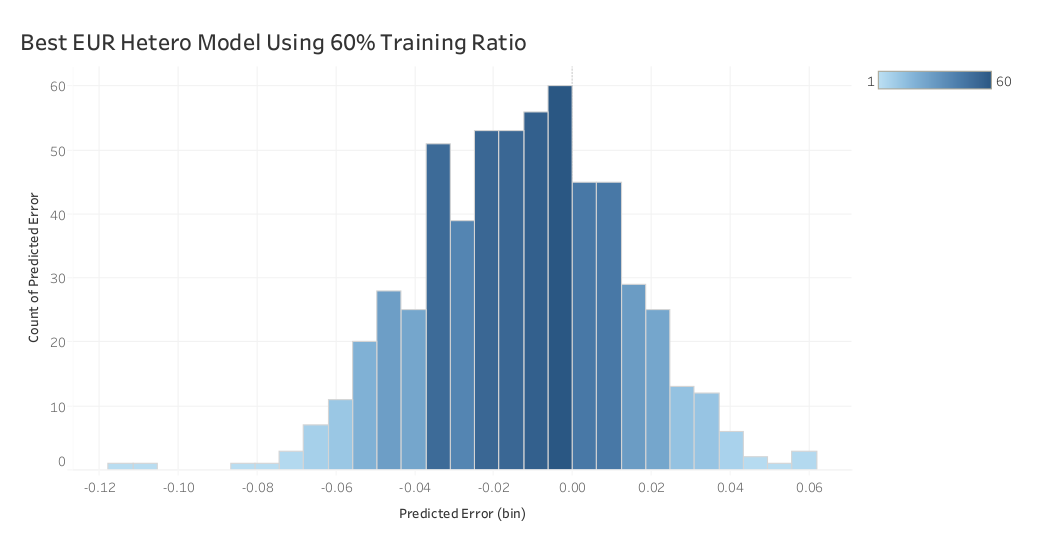
\includegraphics[width=1\textwidth]{hetero_eur_60}
				\caption{The error produced by EUR Hetero model using 60\% training}
			\end{figure}
			\pagebreak
The most errors are lied between -0.01 and 0.01. The following figure compared the actual and predicted values in a line graph manner to demonstrate the difference.
			
			\begin{figure}[hbt!]\centering
				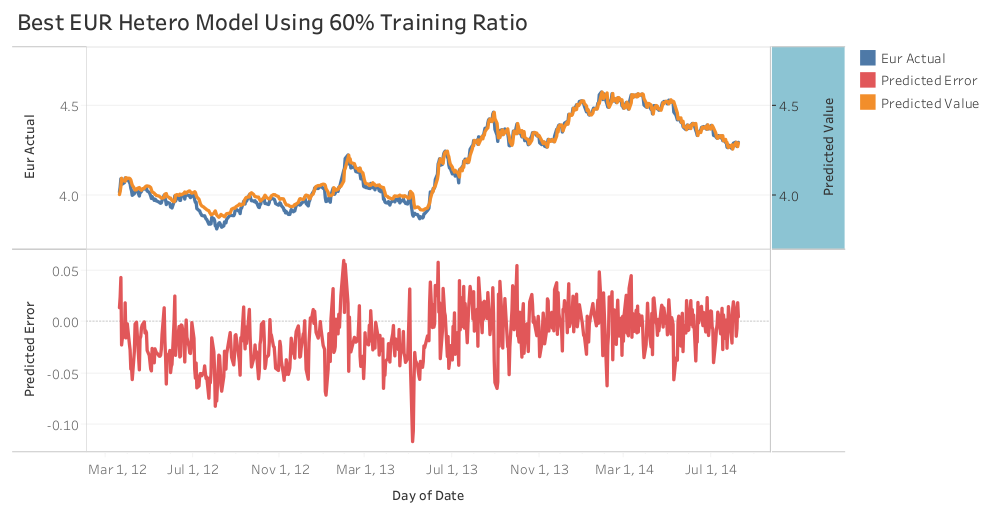
\includegraphics[width=1\textwidth]{best_eur_hetero_APV_60}
				\caption{The error, actual and predicted value produced by EUR Hetero model using 60\% training ratio}
			\end{figure}
			
The table below summarized the outcomes for three training ratio and their best performance of the homogeneous model for EUR currency.
			
			\setlength{\tabcolsep}{0.5em} % for the horizontal padding
			{\renewcommand{\arraystretch}{1.2}
				
				\begin{table}[ht]
					\centering
					\begin{tabular}{@{}rrrrrrrrr@{}}
						\toprule
						\textbf{Ratio}&\textbf{PO}&\textbf{Neurons}& \textbf{RMSE} & \textbf{MAE} & \textbf{Act\_F} & \textbf{Learn\_Rate} &\textbf{ Fus\_Fuc}\\ 
						\midrule
						60\% & 3 & 3 & 0.019668 & 0.015139 & tanh & 0.1 & MAX \\
						70\% & 7 & 8 & 0.022086 & 0.016629 & tanh & 0.1 & MIN \\
						80\% & 5 & 14 & 0.034322 & 0.024755 & tanh & 0.1 & MAX \\
						\hline
					\end{tabular}
					\hspace*{1cm}
					\caption{The three optimal EUR Hetero models with different training ratio}
					
				\end{table}
Among these heterogeneous models, the model which trained with 60\% ratio is the best model which yield the lowest RMSE error rate. The second best optimal model produced is the model which trained with 70\% training datasets ratio. The 80\% training datasets ratio yield the higher RMSE error than compared to other two. Therefore, this 60\% training ratio produced the best reliable accuracy rate compared to both  80\% training ratio  and 70\% training ratio models.

\subsubsection{Ensemble and Single Models}

The optimal two ensemble models for the EUR to RM exchange rate are shown together with the training ratio that yield the optimal models and their predictor order, RMSE, MAE, activation function, learning rate, and fusion function applied.

\begin{table}[ht]
	\centering
	\begin{tabular}{@{}rrrrrrrrrr@{}}
		\toprule
		\textbf{Ensemble} &\textbf{Ratio}&\textbf{PO}&\textbf{Neurons}& \textbf{RMSE} & \textbf{MAE} & \textbf{Act\_F} & \textbf{LR} &\textbf{ Fus\_Fuc}\\ 
		\midrule
		HOMO	& 60\% & 3 & 8 & 0.019116 & 0.014616 & tanh & 0.1 & MIN \\ 	
		HETERO	& 60\% & 3 & 3 & 0.019668 & 0.015139 & tanh & 0.1 & MAX \\
		
		\hline
	\end{tabular}
	\hspace*{1cm}
	\caption{The optimal ensemble  Homo and Hetero models for EUR to RM }
\end{table}

Based on the RMSE rate, the homogeneous ensemble model out perform the heterogeneous model. However, the performance accuracy different for both models is not much, and they both yield better accuracy that current literature accuracy rate for the EUR to RM exchange.

The three  single models for the EUR to RM exchange rate are shown together with the training ratio that yield the optimal models and their predictor order, RMSE, MAE, activation function, and learning rate. Since the homogeneous ensemble yield higher performance accuracy rate, the training parameters from homogeneous model is applied to test in the single models.

\begin{table}[ht]
	\centering
	\begin{tabular}{@{}rrrrrrrrrr@{}}
		\toprule
		\textbf{Single} &\textbf{Ratio}&\textbf{PO}&\textbf{Neurons}& \textbf{RMSE} & \textbf{MAE} & \textbf{Act\_Func} & \textbf{Learn\_Rate} \\ 
		\midrule
			MLP	& 60\% & 3 & 8 & 0.019824 &  0.015608 & tanh & 0.1 \\	
			RNN	& 60\% & 3 & 8 & 0.041590 & 0.035251 & tanh & 0.1 \\
			RBF	& 60\% & 3 & 8 & 0.030003 & 0.0238661 & tanh & 0.1  \\
			\hline
	\end{tabular}
	\hspace*{1cm}
	\caption{The optimal three single models for EUR to RM }
\end{table}

Among these single network models, only MLP yield the reliable accuracy compared to ensemble networks models. Therefore, the homogeneous ensemble model produce the best optimal accuracy among both ensemble and single models.



% GBP CURRENCY
	
\subsection{GBP to RM}
GBP currency exchange rates data is given as inputs to train with homogeneous, and heterogeneous ensemble models using three different training datasets ratio such as 80\%, 70\%, and 60\%. 

\subsubsection{Homogeneous Model}

The results of the model which applied with 80\% of the dataset as training dataset are shown in table 6.9. 

% GBP Train 80%
\setlength{\tabcolsep}{0.5em} % for the horizontal padding
{\renewcommand{\arraystretch}{1.2}
	\begin{table}[ht]
		
		\begin{tabular}{@{}rrrrrrr@{}}
			\toprule
			\textbf{PO}&\textbf{Neurons}& \textbf{RMSE} & \textbf{MAE} & \textbf{Act\_F}  & \textbf{Learn\_Rate} &\textbf{ Fus\_Fuc}\\ 
			\midrule
			 
			  3 & 7 & 0.036700 & 0.026841 & logistic & 0.1 & MAX \\ 
			  4 & 9 & 0.036678 & 0.026946 & tanh & 0.1 & MAX \\ 
			  5 & 5 & 0.036586 & 0.026800 & logistic & 0.1 & MAX \\ 
			  6 & 12 & 0.036625 & 0.026907 & logistic & 0.1 & MAX \\ 
			  7 & 13 & 0.036456 & 0.026894 & logistic & 0.1 & MAX \\ 
			  8 & 9 & 0.036913 & 0.026808 & logistic & 0.1 & MAX \\ 
			  9 & 11 & 0.036546 & 0.027029 & logistic & 0.1 & MAX \\ 
			  10 & 13 & 0.036662 & 0.026970 & logistic & 0.1 & MAX \\ 
			 \hline
			   
			\hline
		\end{tabular}
		\hspace*{1cm}
		\caption{Results On GBP Homogeneous Model Using 80\% Training Ratio }
	\end{table}	
	
	For the 80\% training ratio, the best optimal model  produced 0.038023 RMSE value. The best optimal model which has lowest RMSE error is the predictor order 7 with 13 neurons in the hidden layer with the MAX fusion function. The applied activation function is hyperbolic tangent function with the learning rate of 0.1.
	
	The following histogram explain the minimum and maximum error produced by the best optimal model. The bins of the histogram is 0.0108. The bins is based on the range of error values occurred in each model.
	
	\begin{figure}[hbt!]\centering
		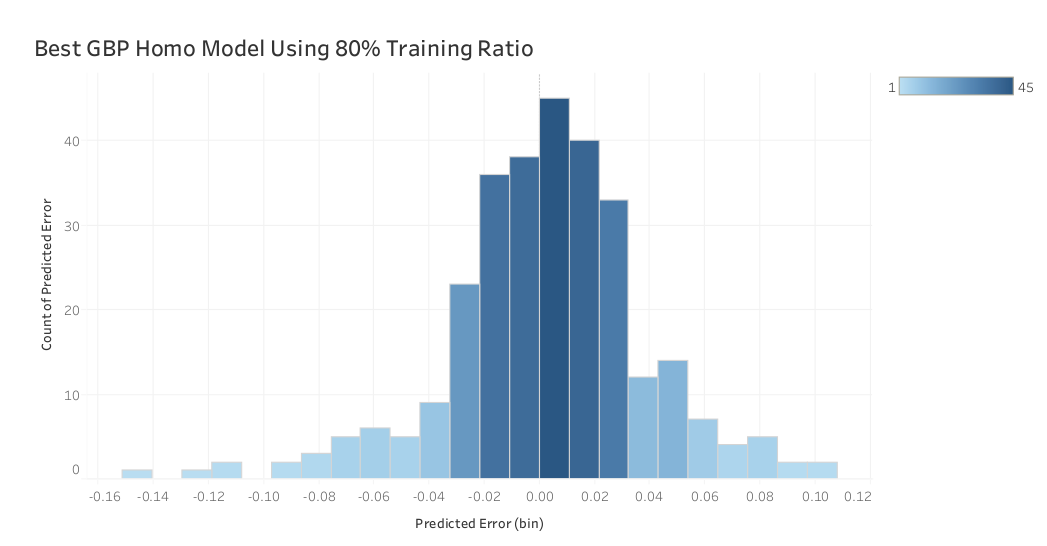
\includegraphics[width=1\textwidth]{homo_gbp_80}
		\caption{The error produced by GBP Homo model using 80\% training ratio}
	\end{figure}
	
	The testing dataset, 10\% of the datasets, has 295 testing results, therefore 295 errors are produced. Among these errors results, the majority of the errors are in between -0.03 and 0.03. There are some outliers with the values between -0.10 and -0.16. The error, actual and predicted value produced by model are shown in graphical manner. The following figure   compared the actual and predicted values in a line graph manner to demonstrate the difference along side with error.
	
	
	\begin{figure}[hbt!]\centering
		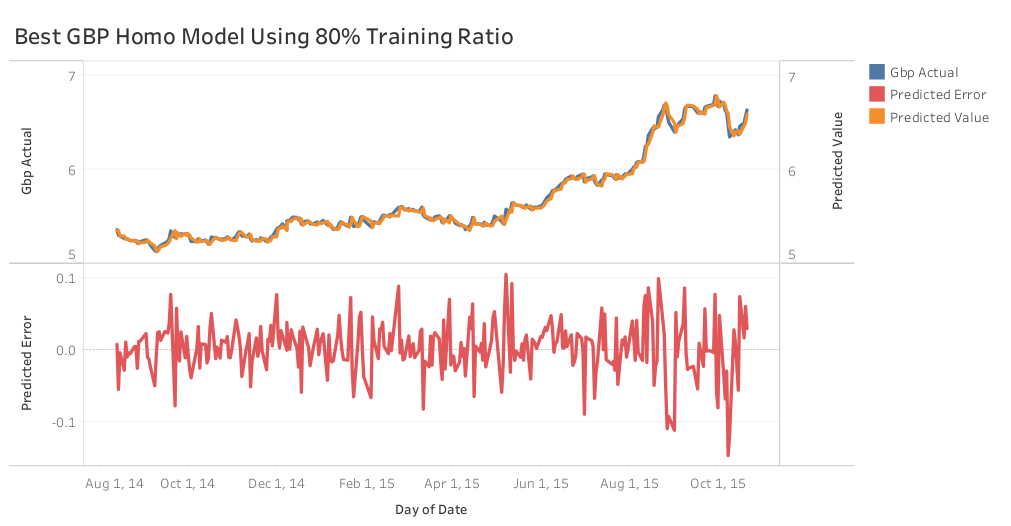
\includegraphics[width=1\textwidth]{best_gbp_homo_APV_80}
		\caption{The error, actual and predicted produced by GBP Homo model  value using 80\% training ratio }
	\end{figure}
	
	
	% EUR Train 70% Need to Modefied
	
	The model which trained with 70\% of the dataset as training dataset are shown in table 6.2. 
	
	\setlength{\tabcolsep}{0.5em} % for the horizontal padding
	{\renewcommand{\arraystretch}{1.2}
		
		\begin{table}[ht]
			\centering
			\begin{tabular}{@{}rrrrrrrr@{}}
				\toprule
				\textbf{PO}&\textbf{Neurons}& \textbf{RMSE} & \textbf{MAE} & \textbf{Act\_F}  & \textbf{Learn\_Rate} &\textbf{ Fus\_Fuc}\\ 
				\midrule
				  3 & 3 & 0.025953 & 0.019841 & logistic & 0.1 & MAX \\ 
				  4 & 5 & 0.026022 & 0.019908 & logistic & 0.1 & MAX \\ 
				  5 & 6 & 0.026114 & 0.019933 & logistic & 0.1 & MAX \\ 
				  6 & 6 & 0.026249 & 0.020033 & tanh & 0.1 & MAX \\ 
				  7 & 4 & 0.025830 & 0.019648 & logistic & 0.1 & MAX \\ 
				  8 & 5 & 0.026165 & 0.019879 & logistic & 0.1 & MAX \\ 
				  9 & 9 & 0.026152 & 0.020108 & logistic & 0.1 & MAX \\ 
				  10 & 6 & 0.025909 & 0.019802 & logistic & 0.1 & MAX \\ 
				\hline 
				
			\end{tabular}
			\hspace*{1cm}
			\caption{Results On GBP Homogeneous Model Using 70\% Training Ratio }
		\end{table}
		
For the model trained with 70\%,  the best optimal model produced 0.025830 RMSE value. The best optimal model which has lowest RMSE error is the predictor order 7 with 4 neurons in the hidden layer with the MAX fusion function. The applied activation function logistic sigmoid function with the learning rate of 0.1.
		
The histogram below explains the minimum and maximum error produced by the best optimal model. The bandwidth of the histogram is 0.0078.
		
		\begin{figure}[hbt!]\centering
			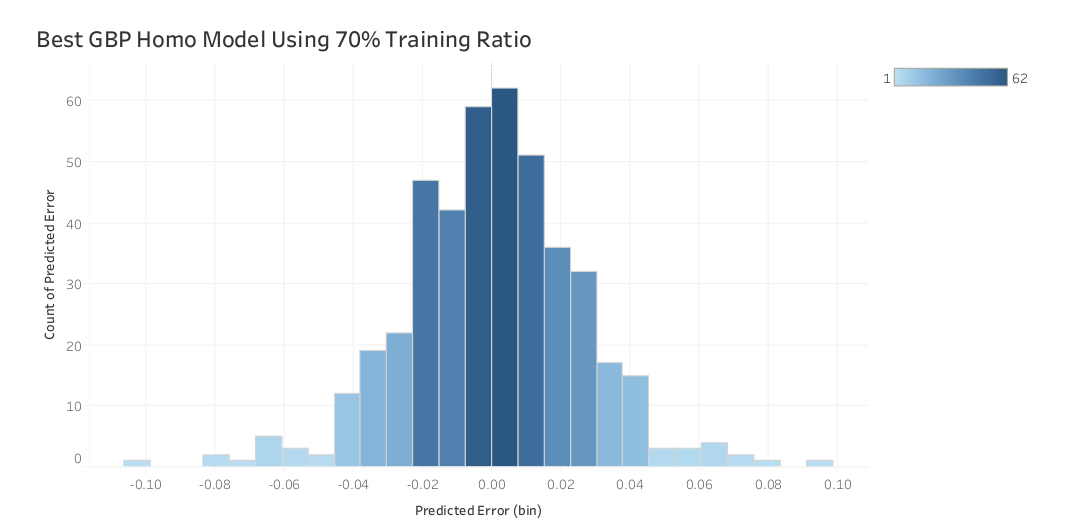
\includegraphics[width=1\textwidth]{homo_gbp_70}
			\caption{The error produced by GBP Homogeneous model  using 70\% training ratio}
		\end{figure}
		
		
The testing dataset, 20\% of the datasets, has 443 experiments, which means 443 errors are yield. The majority of errors are range from -0.03 to 0.04. 
		
		\begin{figure}[hbt!]\centering
			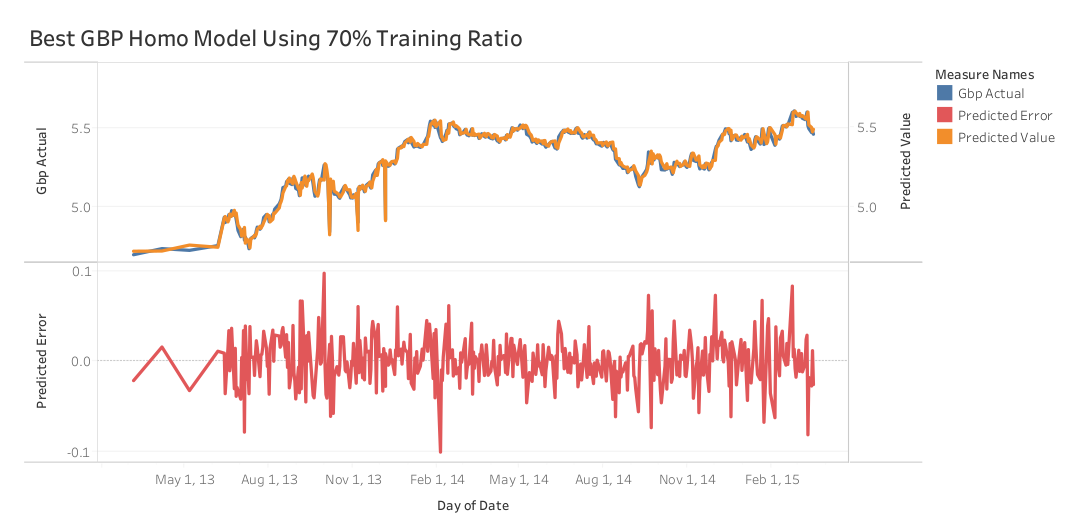
\includegraphics[width=1\textwidth]{best_gbp_homo_APV_70}
			\caption{The error, actual and predicted value produced by GBP Homo model using 70\% training ratio }
		\end{figure}
		\pagebreak
		
The error, actual and predicted value produced by model are shown in following figure in graphical manner.  It can said that the error rate is increased in  Feb 2014, as well as in the early 2015. The model from 70\% training ratio yield better than the model from 80\% training ratio.
		
% GBP Train 60% 
The performance of the model which trained with 60\% of the dataset as training dataset are shown in the following table. 
		
		\setlength{\tabcolsep}{0.5em} % for the horizontal padding
		{\renewcommand{\arraystretch}{1.2}
			\begin{table}[ht]
				\centering
				\begin{tabular}{@{}rrrrrrrr@{}}
					\toprule
					\textbf{PO}&\textbf{Neurons}& \textbf{RMSE} & \textbf{MAE} & \textbf{Act\_F}  & \textbf{Learn\_Rate}&\textbf{ Fus\_Fuc}\\ 
					\midrule
					3 & 6 & 0.022409 & 0.016851 & tanh & 0.1 & MAX \\ 
					4 & 6 & 0.022521 & 0.016944 & tanh & 0.1 & MAX \\ 
					5 & 20 & 0.022654 & 0.017081 & tanh & 0.1 & MAX \\ 
					6 & 6 & 0.022623 & 0.016988 & tanh & 0.1 & MEAN \\ 
					7 & 14 & 0.022622 & 0.017004 & tanh & 0.1 & MAX \\ 
					8 & 7 & 0.022715 & 0.017057 & logistic & 0.1 & MAX \\ 
					9 & 9 & 0.022427 & 0.016876 & logistic & 0.1 & MEAN \\ 
					10 & 9 & 0.022792 & 0.017207 & logistic & 0.1 & MAX \\ 		
					\hline
				\end{tabular}
				\hspace*{1cm}
				\caption{Results On GBP Homogeneous Model Using 60\% Training Ratio}
			\end{table}
			
For the 60\% training datasets applied model, the best optimal model produced 0.022409 RMSE value. The result yield highest  accuracy performance  compared to both the previous models and the current literature result. This model is obtained with the predictor order 3 with 6 neurons in the hidden layer with the MIN fusion function. The applied activation function hyperbolic tangent function with the learning rate of 0.1.
			
The histogram below explains the minimum and maximum error produced by the best optimal model. The bandwidth of the histogram is 0.0071.
			
			\begin{figure}[hbt!]\centering
				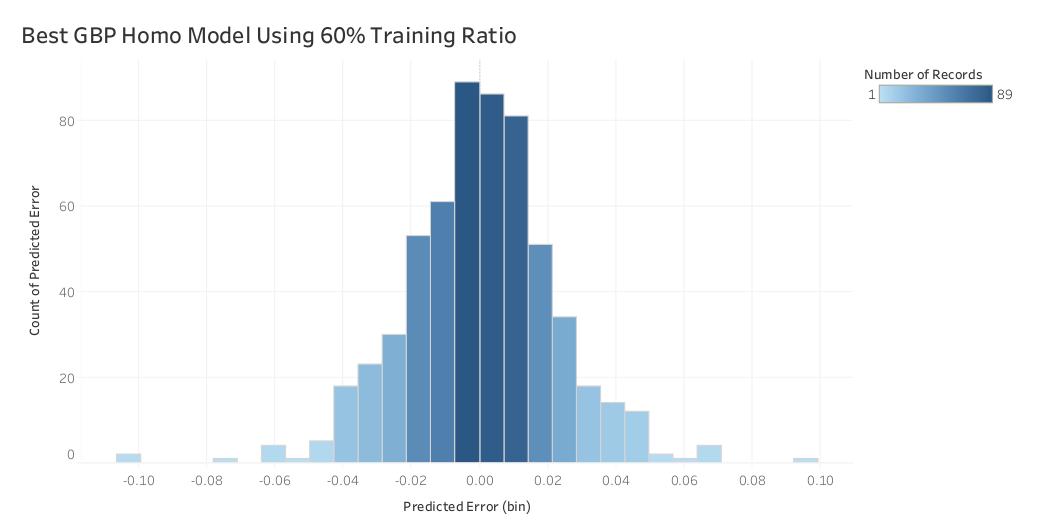
\includegraphics[width=1\textwidth]{homo_gbp_60}
				\caption{The error produced by GBP Homo model using 60\%
					training}
			\end{figure}
			
			\pagebreak
The testing dataset, 20\% of the datasets, has 591 experiments. The most errors are lied between -0.019 and 0.024. The figure below compared the actual and predicted values in a line graph manner to demonstrate the difference.\\
			
			\begin{figure}[hbt!]\centering
				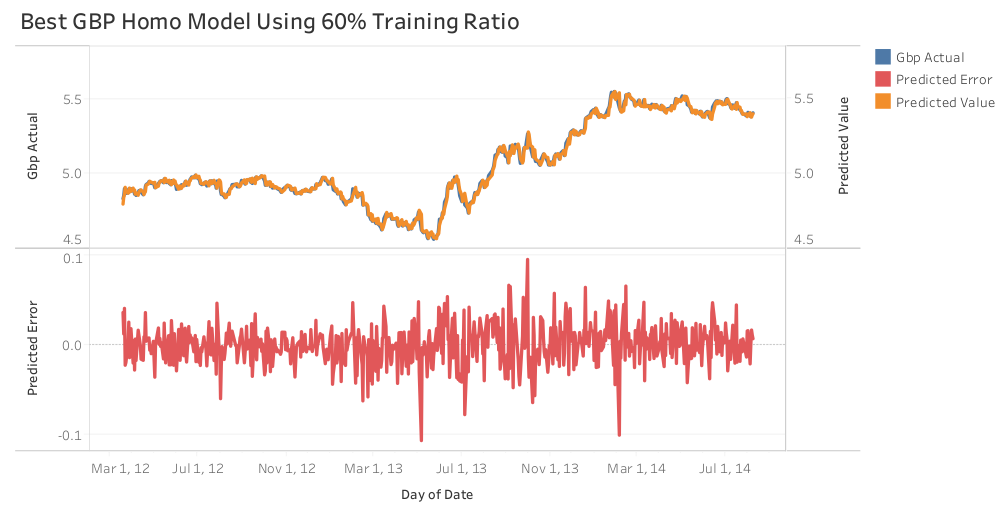
\includegraphics[width=1\textwidth]{best_gbp_homo_APV_60}
				\caption{The error, actual and predicted value produced by GBP Homo model using 60\% training ratio}
			\end{figure}
			\pagebreak
			
			
			The Table 6.12 summarized the outcomes for three training ratio and their best performance of the homogeneous model for GBP currency.
			
			\setlength{\tabcolsep}{0.5em} % for the horizontal padding
			{\renewcommand{\arraystretch}{1.2}
				
				\begin{table}[ht]
					\centering
					\begin{tabular}{@{}rrrrrrrrr@{}}
						\toprule
						\textbf{Ratio}&\textbf{PO}&\textbf{Neurons}& \textbf{RMSE} & \textbf{MAE} & \textbf{Act\_F} & \textbf{Learn\_Rate} &\textbf{ Fus\_Fuc}\\ 
						\midrule
						60\% & 3 & 6 & 0.022409 & 0.016851 & tanh & 0.1 & MAX \\
						70\% & 7 & 4 & 0.025830 & 0.019648 & logistic & 0.1 & MAX \\
						80\% & 7 & 13 & 0.036456 & 0.026894 & logistic & 0.1 & MAX \\
						\hline
					\end{tabular}
					\hspace*{1cm}
					\caption{The three optimal GBP Homo models with different training ratio}
					
				\end{table}
				
Among these homogeneous models, the model which trained with 60\% ratio is the best model which yield the lowest RMSE error rate. The second best optimal model produced is the model which trained with 70\% training datasets ratio. The 80\% training datasets ratio yield the higher RMSE error than compared to other two. Therefore, this 60\% training ratio produced the best reliable accuracy rate compared to both  80\% training ratio  and 70\% training ratio models.

\subsubsection{Heterogeneous Model}

The results of the model which applied to heterogeneous model with 80\% of the dataset as training dataset are shown in table

% EUR Train 80%
\setlength{\tabcolsep}{0.5em} % for the horizontal padding
{\renewcommand{\arraystretch}{1.2}
	\begin{table}[ht]
		
		\begin{tabular}{@{}rrrrrrr@{}}
			\toprule
			\textbf{PO}&\textbf{Neurons}& \textbf{RMSE} & \textbf{MAE} & \textbf{Act\_F} & \textbf{Learn\_Rate}&\textbf{ Fus\_Fuc} \\ 
			\midrule
			3& 15 & 0.043536 & 0.031725 & logistic & 0.1 & MEAN \\ 
			 4 & 5 & 0.046380 & 0.033913 & logistic & 0.1 & MEAN \\ 
			 5 & 6 & 0.046146 & 0.032980 & logistic & 0.1 & MEAN \\ 
			6 & 11 & 0.044436 & 0.031979 & logistic & 0.1 & MEAN \\ 
			 7 & 15 & 0.039117 & 0.028145 & tanh & 0.1 & MAX \\ 
			 8 & 20 & 0.038023 & 0.027797 & tanh & 0.1 & MAX \\ 
			 9 & 11 & 0.040405 & 0.028272 & tanh & 0.1 & MAX \\ 
			 10 & 19 & 0.047473 & 0.035794 & logistic & 0.1 & MEAN \\ 
			\hline
		\end{tabular}
		\hspace*{1cm}
		\caption{Results On GBP Heterogeneous Model Using 80\% Training Ratio }
	\end{table}	
	
For the 80\% training ratio, the best optimal model  produced 0.038023 RMSE value. The best optimal model which has lowest RMSE error is the predictor order 8 with 20 neurons in the hidden layer with the MAX fusion function. The applied activation function is hyperbolic tangent function with the learning rate of 0.1.
	
The following histogram explain the minimum and maximum error produced by the best optimal model. The bins of the histogram is 0.074. The bins is based on the range of error values occurred in each model.
	
	\begin{figure}[hbt!]\centering
		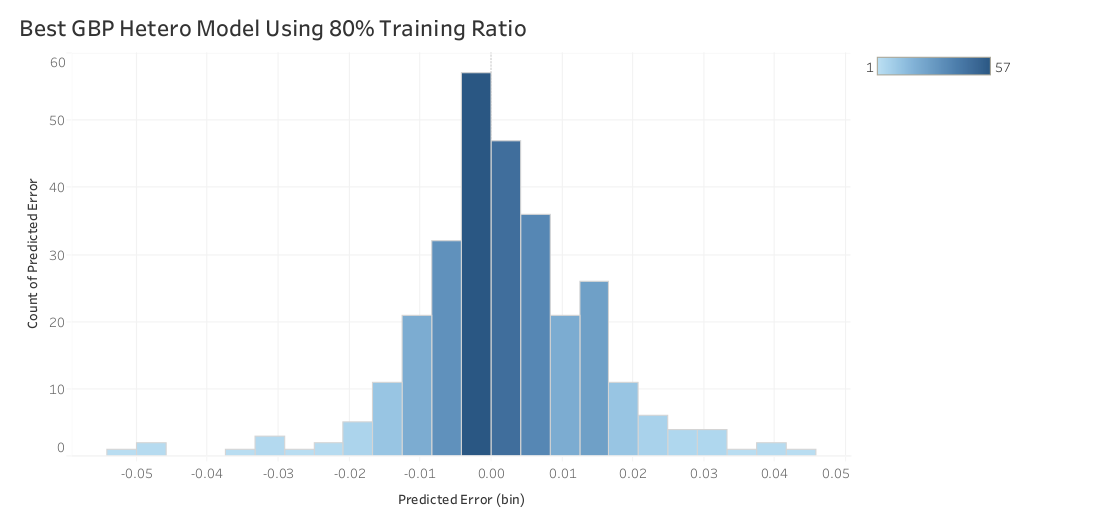
\includegraphics[width=1\textwidth]{hetro_gbp_80}
		\caption{The error produced by GBP Hetro model using 80\% training ratio}
	\end{figure}
	
	
The majority of the errors are in between -0.01 and 0.02. The error, actual and predicted value produced by model are shown  in graphical manner. The following figure compared the actual and predicted values in a line graph manner to demonstrate the difference along side with error.
	
	
	\begin{figure}[hbt!]\centering
		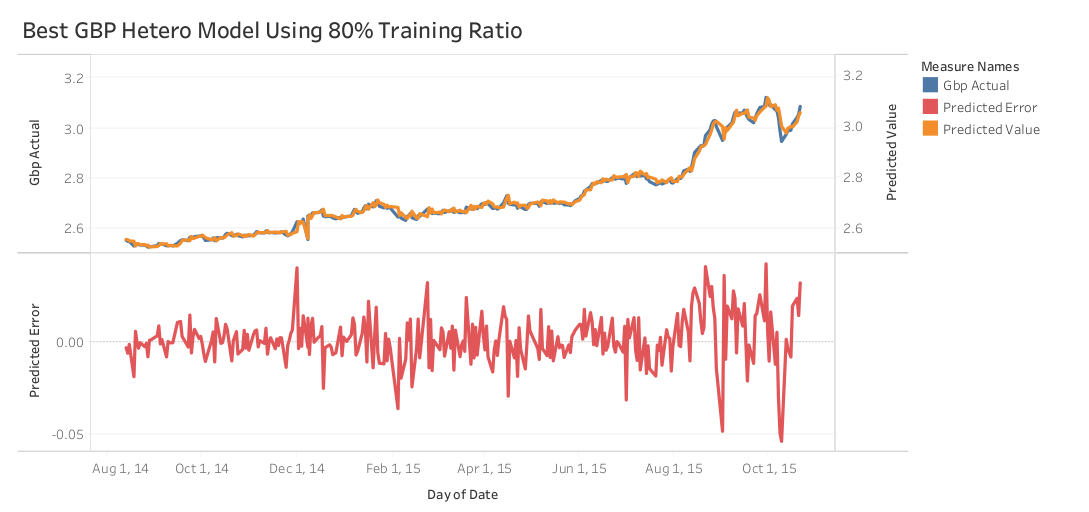
\includegraphics[width=0.9\textwidth]{best_gbp_hetero_APV_80}
		\caption{The error, actual and predicted produced by GBP Hetero model  value using 80\% training ratio }
	\end{figure}
	\pagebreak
	
	% EUR Train 70%
The model which trained with 70\% of the dataset as training dataset are shown in table. Same like the previous ratio, the model is  experimented with 10 predictor orders for the homogeneous model, the optimal model for each predictor order, the number of neurons, RMSE, MAE, activation function and fusion function applied are shown in details.
	
	
	The results of the model which trained with 70\% training dataset ratio is shown in following table.
	
	\setlength{\tabcolsep}{0.5em} % for the horizontal padding
	{\renewcommand{\arraystretch}{1.2}
		
		\begin{table}[ht]
			\centering
			\begin{tabular}{@{}rrrrrrrr@{}}
				\toprule
				\textbf{PO}&\textbf{Neurons}& \textbf{RMSE} & \textbf{MAE} & \textbf{Act\_F}  & \textbf{Learn\_Rate} &\textbf{ Fus\_Fuc}\\ 
				\midrule
				3 & 18 & 0.026537 & 0.020360 & tanh & 0.1 & MAX \\ 
				 4 & 6 & 0.026912 & 0.020816 & tanh & 0.1 & MIN \\ 
				 5 & 4 & 0.026659 & 0.020367 & tanh & 0.1 & MAX \\ 
				 6 & 9 & 0.028075 & 0.021557 & logistic & 0.1 & MAX \\ 
				 7 & 10 & 0.027663 & 0.021140 & tanh & 0.1 & MIN \\ 
				 8 & 5 & 0.027483 & 0.020764 & logistic & 0.1 & MAX \\ 
				 9 & 6 & 0.027099 & 0.020544 & tanh & 0.1 & MAX \\ 
				 10 & 13 & 0.026704 & 0.020137 & tanh & 0.1 & MAX \\ 
				\hline
			\end{tabular}
			\hspace*{1cm}
			\caption{Results On GBP Heterogeneous Model Using 70\% Training Ratio }
		\end{table}
		
For the model trained with 70\%,  the best optimal model produced 0.026537 RMSE value. The best optimal model which has lowest RMSE error is the predictor order 3 with 18 neurons in the hidden layer with the MAX fusion function. The applied activation function hyperbolic tangent function with the learning rate of 0.1.
		
The histogram below explains the minimum and maximum error produced by the best optimal model. The bandwidth of the histogram is 0.0072.
		
		\begin{figure}[hbt!]\centering
			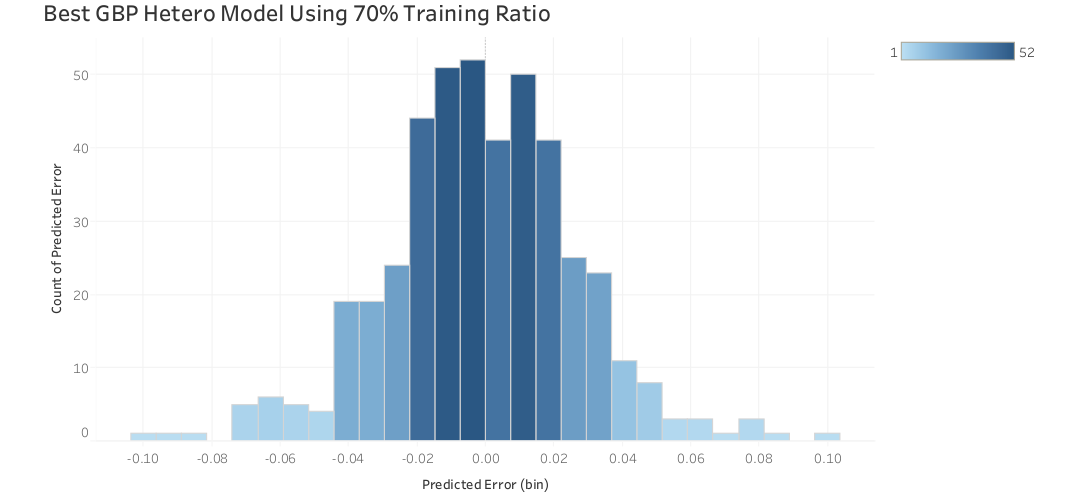
\includegraphics[width=1\textwidth]{best_gbp_hetero_70}
			\caption{The error produced by GBP Hetero model  using 70\% training ratio}
		\end{figure}
		
		The majority of errors are range from -0.04 to 0.04. The error, actual and predicted value produced by model are shown in following figure in graphical manner.  
		\begin{figure}[hbt!]\centering
			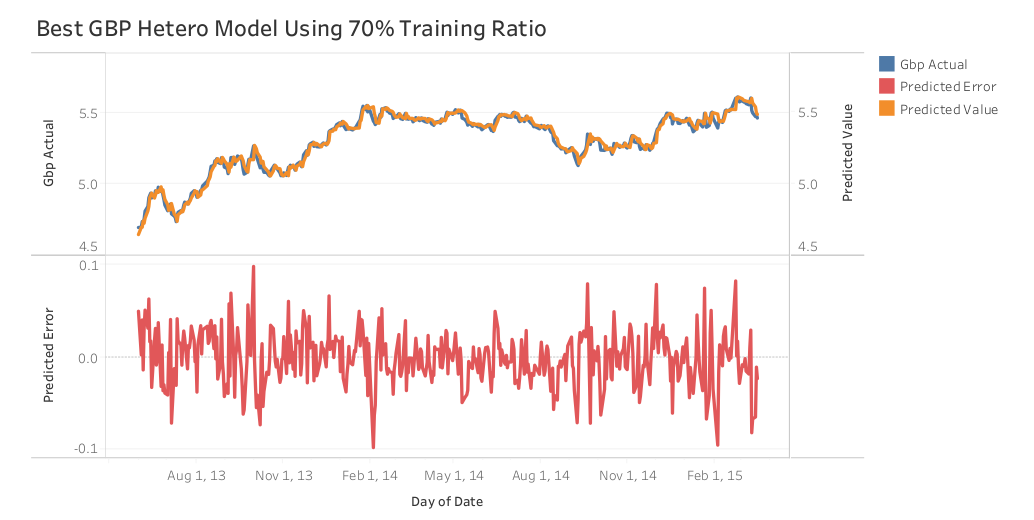
\includegraphics[width=1\textwidth]{best_gbp_hetero_APV_70}
			\caption{The error, actual and predicted value produced by EUR Hetero model using 70\% training ratio }
		\end{figure}
		\pagebreak
		
		% GBP Train 60% 
The model which trained with 60\% of the dataset as training dataset are shown in the following table. Same like the previous ratio, the model is  experimented with 10 predictor orders for the homogeneous model, the optimal model for each predictor order, the number of neurons, RMSE, MAE, activation function and fusion function applied are shown in details. The results of the model which trained with 60\% training dataset ratio is shown in following table.
		\\
		
		\setlength{\tabcolsep}{0.5em} % for the horizontal padding
		{\renewcommand{\arraystretch}{1.2}
			
			\begin{table}[ht]
				\centering
				\begin{tabular}{@{}rrrrrrrr@{}}
					\toprule
					\textbf{PO}&\textbf{Neurons}& \textbf{RMSE} & \textbf{MAE} & \textbf{Act\_F}  & \textbf{Learn\_Rate} &\textbf{ Fus\_Fuc}\\ 
					\midrule
					3 & 6 & 0.022668 & 0.017022 & tanh & 0.1 & MAX \\ 
					 4 & 6 & 0.022505 & 0.016948 & tanh & 0.1 & MAX \\ 
					 5 & 4 & 0.022905 & 0.017253 & tanh & 0.1 & MAX \\ 
					 6 & 20 & 0.022791 & 0.017240 & tanh & 0.1 & MAX \\ 
					 7 & 6 & 0.023118 & 0.017510 & tanh & 0.1 & MAX \\ 
					 8 & 10 & 0.033136 & 0.025481 & tanh & 0.1 & MEAN \\ 
					 9 & 16 & 0.022918 & 0.017395 & tanh & 0.1 & MAX \\ 
					 10 & 18 & 0.022984 & 0.017463 & tanh & 0.1 & MAX \\ 
					\hline
				\end{tabular}
				\hspace*{1cm}
				\caption{Results On GBP Heterogeneous Model Using 60\% Training Ratio}
			\end{table}
			
For the 60\% training datasets applied model, the best optimal model produced 0.022505 RMSE value.  This model is obtained with the predictor order 4 with 6 neurons in the hidden layer with the MAX fusion function. The applied activation function hyperbolic tangent function with the learning rate of 0.1.
			
The histogram below explains the minimum and maximum error produced by the best optimal model. The bandwidth of the histogram is 0.0042.
			
			\begin{figure}[hbt!]\centering
				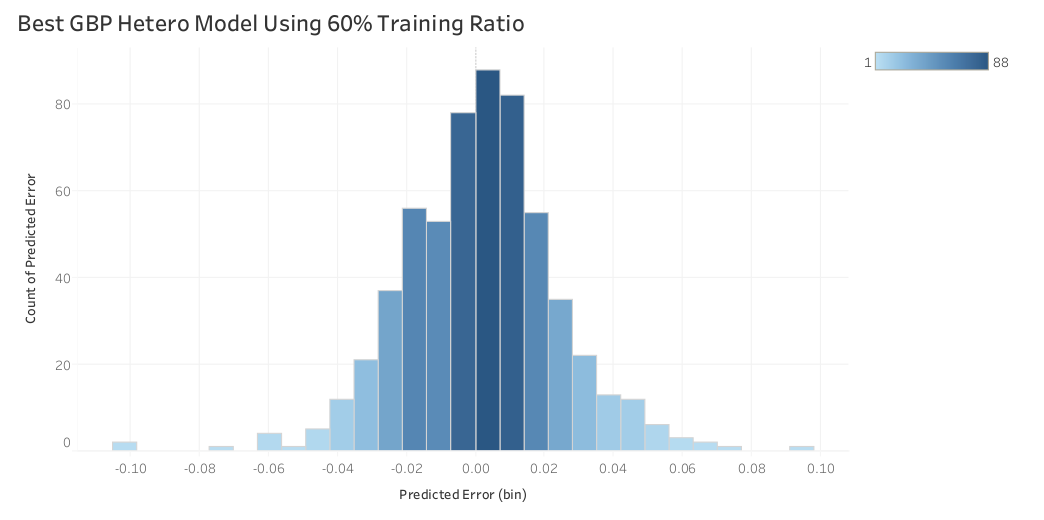
\includegraphics[width=1\textwidth]{hetero_gbp_60}
				\caption{The error produced by GBP Hetero model using 60\% training}
			\end{figure}
			
The most errors are lied between -0.02 and 0.03. The following figure compared the actual and predicted values in a line graph manner to demonstrate the difference.
			
			\begin{figure}[hbt!]\centering
				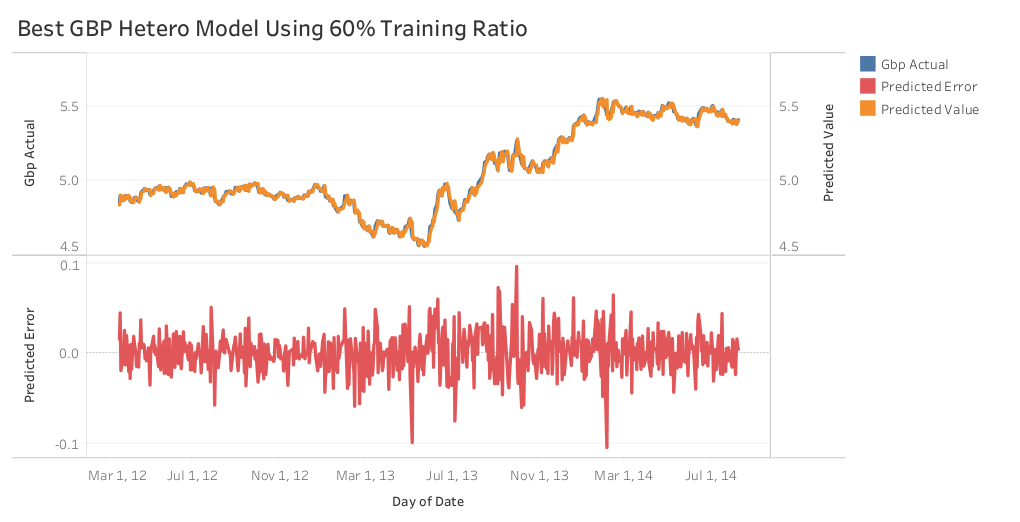
\includegraphics[width=1\textwidth]{best_gbp_hetero_APV_60}
				\caption{The error, actual and predicted value produced by EUR Hetero model using 60\% training ratio}
			\end{figure}
			\pagebreak
			The table below summarized the outcomes for three training ratio and their best performance of the homogeneous model for GBP currency.
			
			\setlength{\tabcolsep}{0.5em} % for the horizontal padding
			{\renewcommand{\arraystretch}{1.2}
				
				\begin{table}[ht]
					\centering
					\begin{tabular}{@{}rrrrrrrrr@{}}
						\toprule
						\textbf{Ratio}&\textbf{PO}&\textbf{Neurons}& \textbf{RMSE} & \textbf{MAE} & \textbf{Act\_F} & \textbf{Learn\_Rate} &\textbf{ Fus\_Fuc}\\ 
						\midrule
						60\% & 4 & 6 & 0.022505 & 0.016948 & tanh & 0.1 & MAX \\  
						70\% & 3 & 18 & 0.026537 & 0.020360 & tanh & 0.1 & MAX \\ 
						80\% & 8 & 20 & 0.038023 & 0.027797 & tanh & 0.1 & MAX \\ 
						\hline
					\end{tabular}
					\hspace*{1cm}
					\caption{The three optimal GBP Hetero models with different training ratio}
					
				\end{table}
				Among these heterogeneous models, the model which trained with 60\% ratio is the best model which yield the lowest RMSE error rate. The second best optimal model produced is the model which trained with 70\% training datasets ratio. The 80\% training datasets ratio yield the higher RMSE error than compared to other two. Therefore, this 60\% training ratio produced the best reliable accuracy rate compared to both  80\% training ratio  and 70\% training ratio models.
				

\subsubsection{Ensemble and Single Models}

The optimal two ensemble models for the GBP to RM exchange rate are shown together with the training ratio that yield the optimal models and their predictor order, RMSE, MAE, activation function, learning rate, and fusion function applied.

\begin{table}[ht]
	\centering
	\begin{tabular}{@{}rrrrrrrrrr@{}}
		\toprule
		\textbf{Ensemble} &\textbf{Ratio}&\textbf{PO}&\textbf{Neurons}& \textbf{RMSE} & \textbf{MAE} & \textbf{Act\_F} & \textbf{LR} &\textbf{ Fus\_Fuc}\\ 
		\midrule
			HOMO	& 60\% & 3 & 6 & 0.022409 & 0.016851 & tanh & 0.1 & MAX \\
			HETERO	& 60\% & 4 & 6 & 0.022505 & 0.016948 & tanh & 0.1 & MAX \\ 
			
			\hline
		\end{tabular}
		\hspace*{1cm}
		\caption{The optimal Ensemble  Homo and Hetero models for GBP to RM }
\end{table}

Based on the RMSE rate, the homogeneous ensemble model out perform the heterogeneous model. However, the performance accuracy different for both models is not much, and they both yield better accuracy that current literature accuracy rate for the GBP to RM exchange.

The three  single models for the GBP to RM exchange rate are shown together with the training ratio that yield the optimal models and their predictor order, RMSE, MAE, activation function, and learning rate. Since the homogeneous ensemble yield higher performance accuracy rate, the training parameters from homogeneous model is applied to test in the single models.

\begin{table}[ht]
	\centering
	\begin{tabular}{@{}rrrrrrrrrr@{}}
		\toprule
		\textbf{Single} &\textbf{Ratio}&\textbf{PO}&\textbf{Neurons}& \textbf{RMSE} & \textbf{MAE} & \textbf{Act\_Func} & \textbf{Learn\_Rate} \\ 
		\midrule
		MLP	& 60\% & 3 & 6 & 0.022430 &  0.016852 & tanh & 0.1 \\	
		RNN	& 60\% & 3 & 6 & 0.056163 & 0.049153 & tanh & 0.1 \\
		RBF	& 60\% & 3 & 6 & 0.040494 & 0.030088 & tanh & 0.1  \\
		\hline
	\end{tabular}
	\hspace*{1cm}
	\caption{The optimal three single models for GBP to RM }
\end{table}

Among these single network models, only MLP yield the reliable accuracy compared to ensemble networks models. Therefore, the homogeneous ensemble model produce the best optimal accuracy among both ensemble and single models.


% SGD CURRENCY 
\subsection{SGD to RM}

SGD currency exchange rates data is given as inputs to train with homogeneous, and heterogeneous ensemble models using three different training datasets ratio such as 80\%, 70\%, and 60\%. 

\subsubsection{Homogeneous Model}

The results of the model which applied with 80\% of the dataset as training dataset are shown in the table. 

% SGD Train 80%
\setlength{\tabcolsep}{0.5em} % for the horizontal padding
{\renewcommand{\arraystretch}{1.2}
	\begin{table}[ht]
		
		\begin{tabular}{@{}rrrrrrr@{}}
			\toprule
			\textbf{PO}&\textbf{Neurons}& \textbf{RMSE} & \textbf{MAE} & \textbf{Act\_F}  & \textbf{Learn\_Rate} &\textbf{ Fus\_Fuc}\\ 
			\midrule
			
			 3 & 15 & 0.012557 & 0.008928 & tanh & 0.1 & MAX \\ 
			 4 & 18 & 0.013140 & 0.009256 & tanh & 0.1 & MAX \\ 
			 5 & 6 & 0.013093 & 0.009158 & tanh & 0.1 & MAX \\ 
			 6 & 12 & 0.013203 & 0.009272 & tanh & 0.1 & MAX \\ 
			 7 & 14 & 0.014963 & 0.010255 & tanh & 0.1 & MAX \\ 
			 8 & 14 & 0.014300 & 0.009966 & tanh & 0.1 & MAX \\ 
			 9 & 19 & 0.019807 & 0.012714 & tanh & 0.1 & MAX \\ 
			 10 & 13 & 0.017241 & 0.011438 & tanh & 0.1 & MAX \\ 
		
			\hline
		\end{tabular}
		\hspace*{1cm}
		\caption{Results On SGD Homogeneous Model Using 80\% Training Ratio }
	\end{table}	
	
	
For the 80\% training ratio, the best optimal model  produced 0.012557 RMSE value. The best optimal model which has lowest RMSE error is the predictor order 3 with 15 neurons in the hidden layer with the MAX fusion function. The applied activation function is hyperbolic tangent function with the learning rate of 0.1.
	
	The following histogram explain the minimum and maximum error produced by the best optimal model. The bins of the histogram is 0.00387. The bins is based on the range of error values occurred in each model.
	
	\begin{figure}[hbt!]\centering
		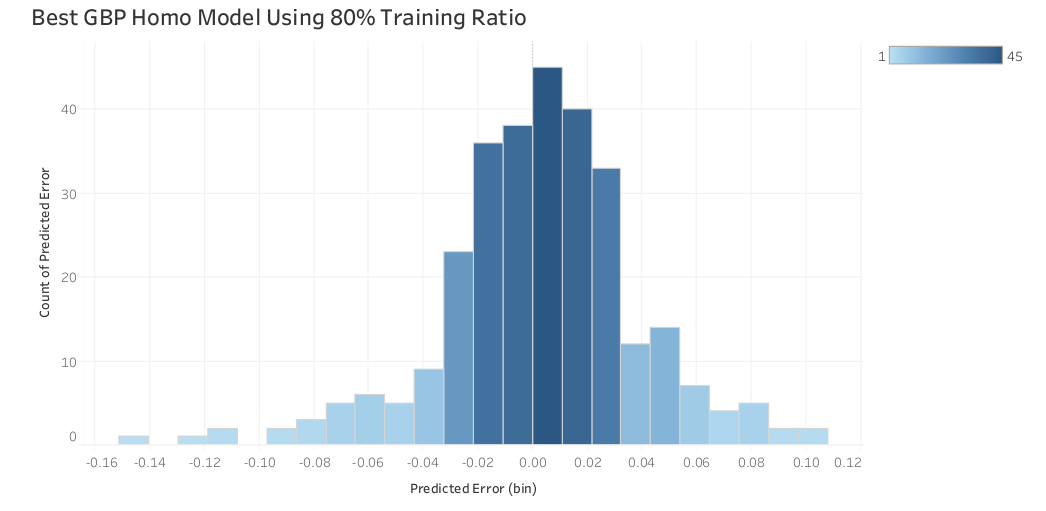
\includegraphics[width=1\textwidth]{homo_sgd_80}
		\caption{The error produced by SGD Homo model using 80\% training ratio}
	\end{figure}
	\pagebreak
The testing dataset, 10\% of the datasets, has 295 testing results, therefore 295 errors are produced. Among these errors results, the majority of the errors are in between -0.018 and 0.018. There are some outliers with the values between -0.12 and -0.16. The error, actual and predicted value produced by model are shown in graphical manner. The following figure   compared the actual and predicted values in a line graph manner to demonstrate the difference along side with error.
	
	
	\begin{figure}[hbt!]\centering
		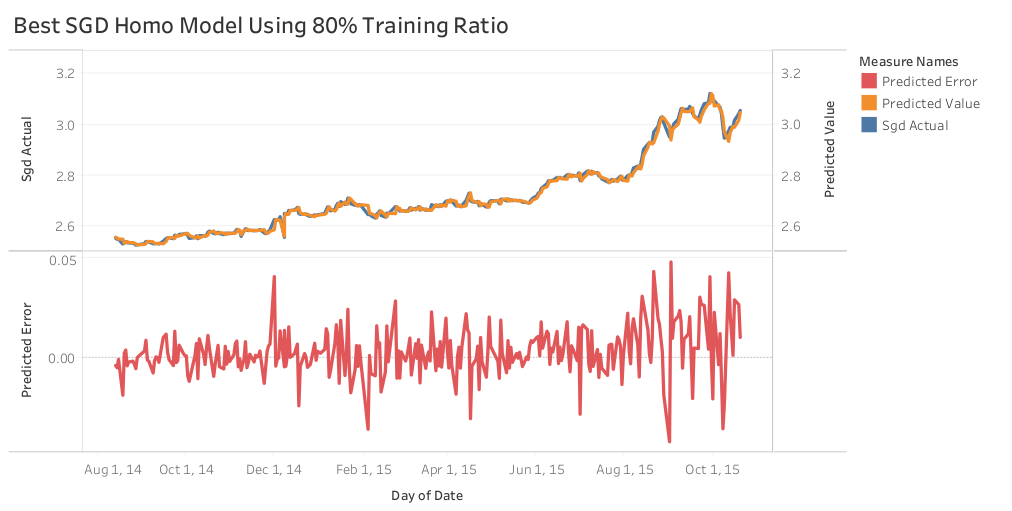
\includegraphics[width=0.9\textwidth]{best_sgd_homo_APV_80}
		\caption{The error, actual and predicted produced by SGD Homo model  value using 80\% training ratio }
	\end{figure}
	
	
	\pagebreak 
	
% SGD Train 70% 
	
The model which trained with 70\% of the dataset as training dataset are shown in table.
	
	\setlength{\tabcolsep}{0.5em} % for the horizontal padding
	{\renewcommand{\arraystretch}{1.2}
		
		\begin{table}[ht]
			\centering
			\begin{tabular}{@{}rrrrrrrr@{}}
				\toprule
				\textbf{PO}&\textbf{Neurons}& \textbf{RMSE} & \textbf{MAE} & \textbf{Act\_F}  & \textbf{Learn\_Rate} &\textbf{ Fus\_Fuc}\\ 
				\midrule
				
				 3 & 11& 0.007860 & 0.005687 & tanh & 0.1 & MAX \\ 
				 4 & 3 & 0.007889 & 0.005745 & tanh & 0.1 & MEAN \\ 
				 5 & 6 & 0.007872 & 0.005764 & tanh & 0.1 & MAX \\ 
				 6 & 12 & 0.007917 & 0.005744 & tanh & 0.1 & MAX \\ 
				 7 & 12 & 0.007937 & 0.005868 & tanh & 0.1 & MAX \\ 
				 8 & 14 & 0.007984 & 0.005864 & logistic & 0.1 & MAX \\ 
				 9 & 8 & 0.008066 & 0.005892 & logistic & 0.1 & MAX \\ 
				 10 & 18 & 0.007926 & 0.005811 & logistic & 0.1 & MAX \\ 
				
				\hline 
				
			\end{tabular}
			\hspace*{1cm}
			\caption{Results On SGD Homogeneous Model Using 70\% Training Ratio }
		\end{table}
		
For the model trained with 70\%, the best optimal model produced 0.007860 RMSE value. The best optimal model which has lowest RMSE error is the predictor order 3 with 11 neurons in the hidden layer with the MAX fusion function. The applied activation function logistic sigmoid function with the learning rate of 0.1.
		
The histogram below explains the minimum and maximum error produced by the best optimal model. The bandwidth of the histogram is 0.00295.
		
		\begin{figure}[hbt!]\centering
			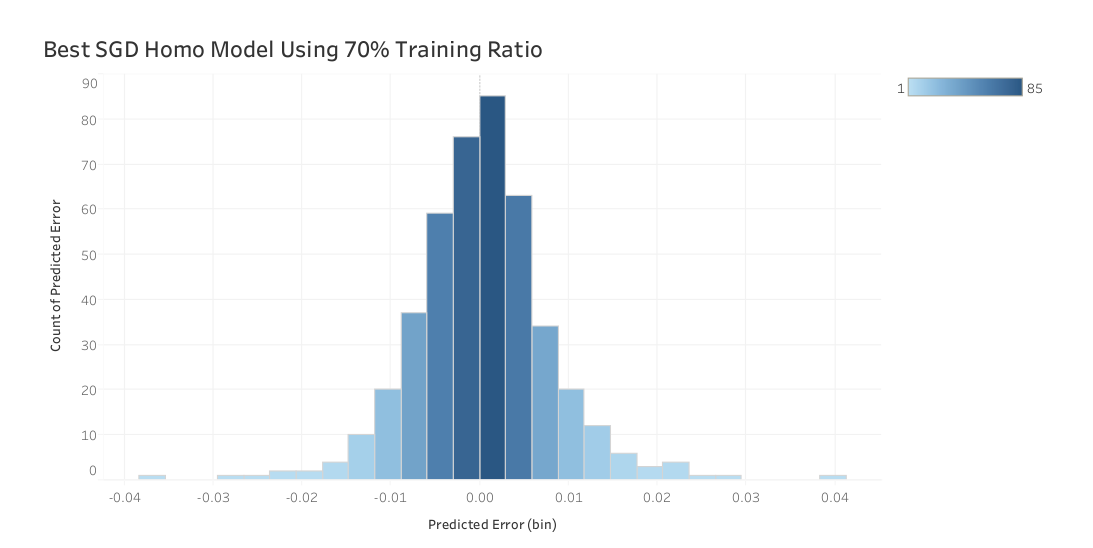
\includegraphics[width=0.9\textwidth]{homo_sgd_70}
			\caption{The error produced by SGD Homogeneous model  using 70\% training ratio}
		\end{figure}
		\pagebreak
		
The testing dataset, 20\% of the datasets, has 443 experiments, which means 443 errors are yield. The majority of errors are range from -0.005 to 0.007. 
		
		\begin{figure}[hbt!]\centering
			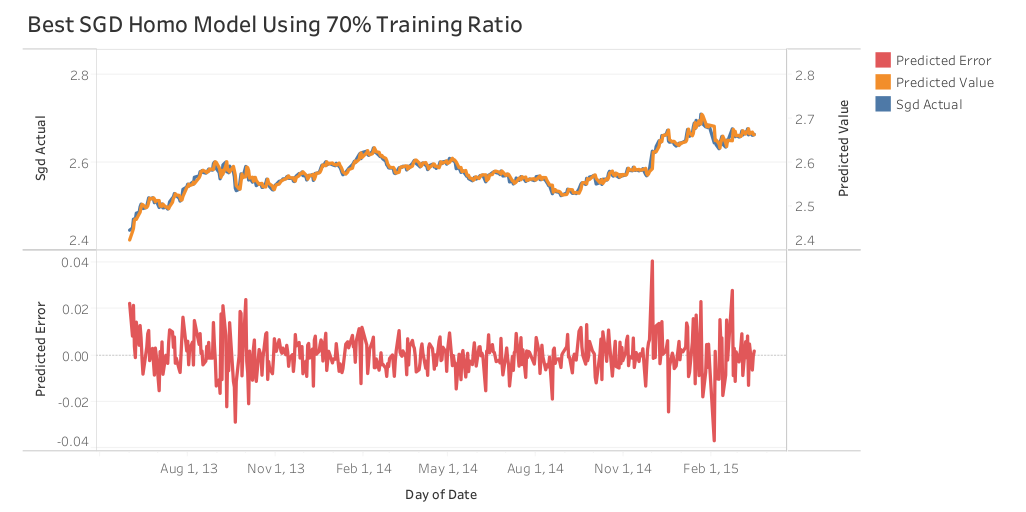
\includegraphics[width=0.9\textwidth]{best_sgd_homo_APV_70}
			\caption{The error, actual and predicted value produced by SGD Homo model using 70\% training ratio }
		\end{figure}
		
		
The error, actual and predicted value produced by model are in graphical manner.  It can said that the error rate is increased in  October 2013, as well as in the early 2015. The model from 70\% training ratio yield better than the model from 80\% training ratio.
		
% SGD Train 60% 
The performance of the model which trained with 60\% of the dataset as training dataset are shown in the following table. 
		
		\setlength{\tabcolsep}{0.5em} % for the horizontal padding
		{\renewcommand{\arraystretch}{1.2}
			\begin{table}[ht]
				\centering
				\begin{tabular}{@{}rrrrrrrr@{}}
					\toprule
					\textbf{PO}&\textbf{Neurons}& \textbf{RMSE} & \textbf{MAE} & \textbf{Act\_F}  & \textbf{Learn\_Rate}&\textbf{ Fus\_Fuc}\\ 
					\midrule
					3 & 5 & 0.006562 & 0.004605 & tanh & 0.1 & MAX \\ 
					4 & 13 & 0.006566 & 0.004640 & tanh & 0.1 & MAX \\ 
					5 & 3 & 0.006774 & 0.004754 & tanh & 0.1 & MAX \\ 
					6 & 7 & 0.006679 & 0.004729 & tanh & 0.1 & MAX \\ 
					7 & 11 & 0.006652 & 0.004770 & tanh & 0.1 & MAX \\ 
					8 & 13 & 0.006564 & 0.004666 & tanh & 0.1 & MAX \\ 
					9 & 13 & 0.006794 & 0.004837 & logistic & 0.1 & MAX \\ 
					10 & 17 & 0.006710 & 0.004772 & tanh & 0.1 & MEAN \\ 
					
					\hline
				\end{tabular}
				\hspace*{1cm}
				\caption{Results On SGD Homogeneous Model Using 60\% Training Ratio}
			\end{table}
			\pagebreak
For the 60\% training datasets applied model, the best optimal model produced 0.006562 RMSE value. The result yield highest  accuracy performance  compared to both the previous models and the current literature result. This model is obtained with the predictor order 3 with 5 neurons in the hidden layer with the MIN fusion function. The applied activation function hyperbolic tangent function with the learning rate of 0.1.
			
The histogram below explains the minimum and maximum error produced by the best optimal model. The bandwidth of the histogram is 0.00281.
			
			\begin{figure}[hbt!]\centering
				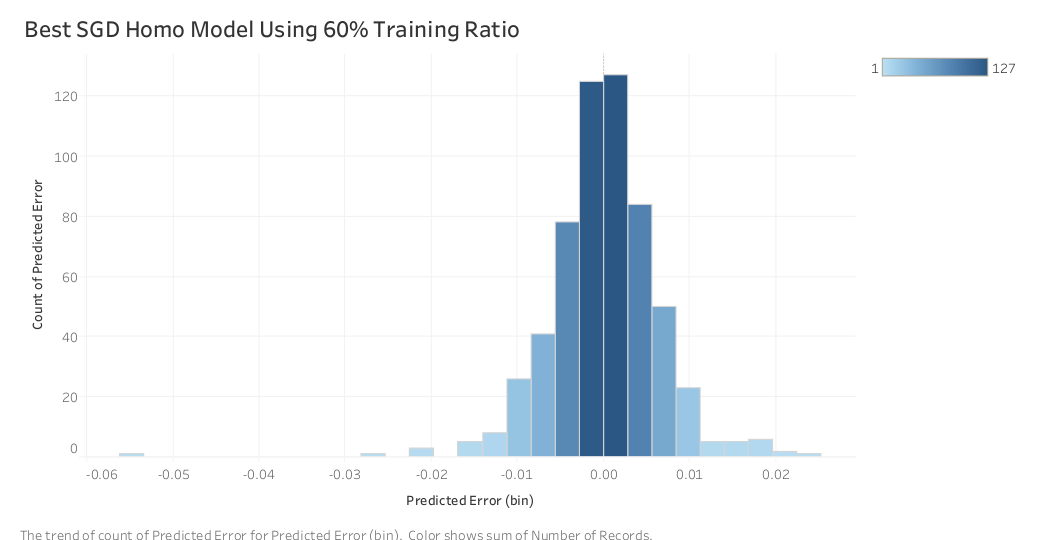
\includegraphics[width=1\textwidth]{homo_sgd_60}
				\caption{The error produced by SGD Homo model using 60\%
					training}
			\end{figure}
			
			
The testing dataset, 20\% of the datasets, has 591 experiments. The most errors are lied between -0.01 and 0.01. The figure below compared the actual and predicted values in a line graph manner to demonstrate the difference.\\
			
			\begin{figure}[hbt!]\centering
				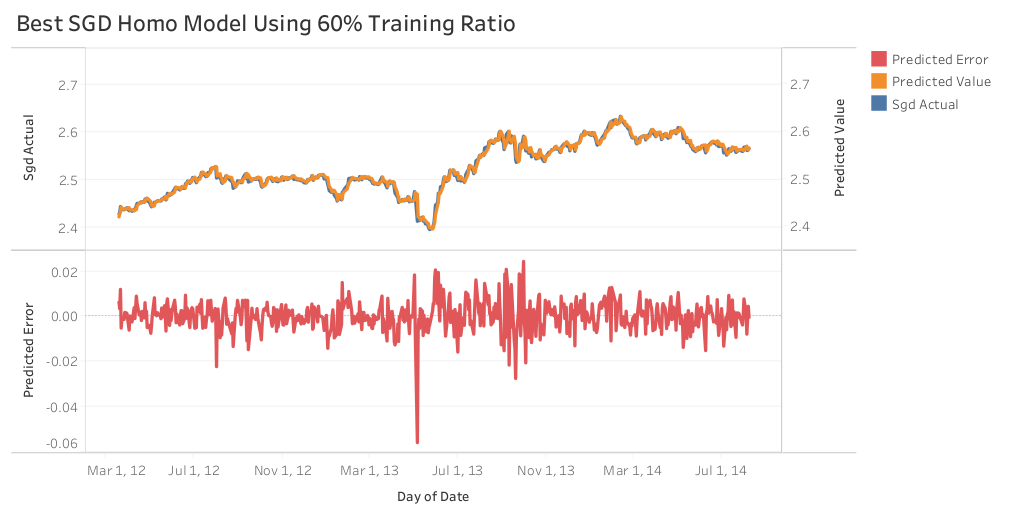
\includegraphics[width=1\textwidth]{best_sgd_homo_APV_60}
				\caption{The error, actual and predicted value produced by SGD Homo model using 60\% training ratio}
			\end{figure}
			\pagebreak
			
			
The Table 6.16 summarized the outcomes for three training ratio and their best performance of the homogeneous model for SGD currency.
			
			\setlength{\tabcolsep}{0.5em} % for the horizontal padding
			{\renewcommand{\arraystretch}{1.2}
				
				\begin{table}[ht]
					\centering
					\begin{tabular}{@{}rrrrrrrrr@{}}
						\toprule
						\textbf{Ratio}&\textbf{PO}&\textbf{Neurons}& \textbf{RMSE} & \textbf{MAE} & \textbf{Act\_F} & \textbf{Learn\_Rate} &\textbf{ Fus\_Fuc}\\ 
						\midrule
						60\% & 3 & 5 & 0.006562 & 0.004605 & tanh & 0.1 & MAX \\
						70\% & 3 & 11& 0.007860 & 0.005687 & tanh & 0.1 & MAX \\ 
						80\% & 3 & 15 & 0.012557 & 0.008928 & tanh & 0.1 & MAX \\ 
						\hline
					\end{tabular}
					\hspace*{1cm}
					\caption{The three optimal SGD Homo models with different training ratio}
					
				\end{table}
				
Among these homogeneous models, the model which trained with 60\% ratio is the best model which yield the lowest RMSE error rate. The second best optimal model produced is the model which trained with 70\% training datasets ratio. The 80\% training datasets ratio yield the higher RMSE error than compared to other two. Therefore, this 60\% training ratio produced the best reliable accuracy rate compared to both  80\% training ratio  and 70\% training ratio models.
				
\subsubsection{Heterogeneous Model}

The results of the model which applied to heterogeneous model with 80\% of the dataset as training dataset are shown in table

% SGD Train 80%
\setlength{\tabcolsep}{0.5em} % for the horizontal padding
{\renewcommand{\arraystretch}{1.2}
	\begin{table}[ht]
		
		\begin{tabular}{@{}rrrrrrr@{}}
			\toprule
			\textbf{PO}&\textbf{Neurons}& \textbf{RMSE} & \textbf{MAE} & \textbf{Act\_F} & \textbf{Learn\_Rate}&\textbf{ Fus\_Fuc} \\ 
			\midrule
			3 & 16 & 0.016432 & 0.011504 & tanh & 0.1 & MEAN \\ 
			4 & 18 & 0.013209 & 0.009360 & tanh & 0.1 & MAX \\ 
			 5 & 6 & 0.013063 & 0.009322 & tanh & 0.1 & MAX \\ 
			 6 & 4 & 0.019550 & 0.012832 & tanh & 0.1 & MAX \\ 
			 7 & 12 & 0.016472 & 0.011410 & tanh & 0.1 & MAX \\ 
			 8 & 20 & 0.013087 & 0.009369 & tanh & 0.1 & MAX \\ 
			 9 & 6 & 0.026961 & 0.016779 & tanh & 0.1 & MAX \\ 
			 10 & 11 & 0.022162 & 0.016224 & tanh & 0.1 & MEAN \\ 
			\hline
		\end{tabular}
		\hspace*{1cm}
		\caption{Results On SGD Heterogeneous Model Using 80\% Training Ratio }
	\end{table}	
	
For the 80\% training ratio, the best optimal model  produced 0.013063 RMSE value. The best optimal model which has lowest RMSE error is the predictor order 5 with 6 neurons in the hidden layer with the MAX fusion function. The applied activation function is hyperbolic tangent function with the learning rate of 0.1.
	
The following histogram explain the minimum and maximum error produced by the best optimal model. The bins of the histogram is 0.0361. The bins is based on the range of error values occurred in each model.
	
	\begin{figure}[hbt!]\centering
		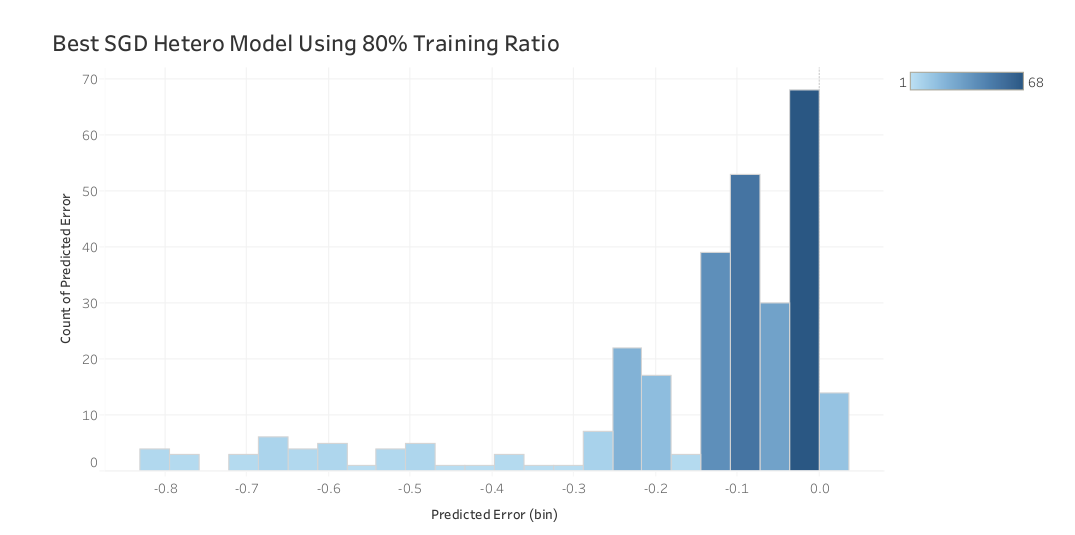
\includegraphics[width=1\textwidth]{hetro_sgd_80}
		\caption{The error produced by SGD Hetro model using 80\% training ratio}
	\end{figure}
\pagebreak
	
	
The majority of the errors are in between -0.015 and 0.01. The error, actual and predicted value produced by model are shown  in graphical manner. The following figure compared the actual and predicted values in a line graph manner to demonstrate the difference along side with error.
	
	
	\begin{figure}[hbt!]\centering
		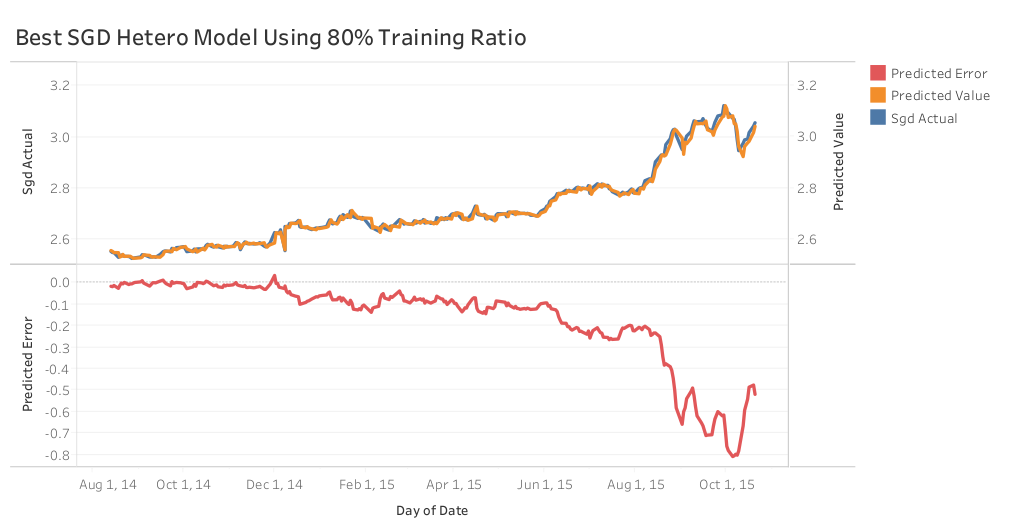
\includegraphics[width=0.9\textwidth]{best_sgd_hetero_APV_80}
		\caption{The error, actual and predicted produced by SGD Hetero model  value using 80\% training ratio }
	\end{figure}
	\pagebreak
	
% SGD Train 70%
	
The model which trained with 70\% of the dataset as training dataset are shown in table. Same like the previous ratio, the model is  experimented with 10 predictor orders for the homogeneous model, the optimal model for each predictor order, the number of neurons, RMSE, MAE, activation function and fusion function applied are shown in details.
	
	
The results of the model which trained with 70\% training dataset ratio is shown in following table.
	
	\setlength{\tabcolsep}{0.5em} % for the horizontal padding
	{\renewcommand{\arraystretch}{1.2}
		
		\begin{table}[ht]
			\centering
			\begin{tabular}{@{}rrrrrrrr@{}}
				\toprule
				\textbf{PO}&\textbf{Neurons}& \textbf{RMSE} & \textbf{MAE} & \textbf{Act\_F}  & \textbf{Learn\_Rate} &\textbf{ Fus\_Fuc}\\ 
				\midrule
				 3 & 14 & 0.008317 & 0.006099 & tanh & 0.1 & MAX \\ 
				 4 & 11 & 0.008487 & 0.006285 & tanh & 0.1 & MAX \\ 
				 5 & 5 & 0.008279 & 0.006066 & tanh & 0.1 & MAX \\ 
				 6 & 16 & 0.009038 & 0.006943 & tanh & 0.1 & MEAN \\ 
				 7 & 5 & 0.008646 & 0.006325 & tanh & 0.1 & MAX \\ 
				 8 & 20 & 0.008423 & 0.006172 & tanh & 0.1& MAX \\ 
				 9 & 16 & 0.009094 & 0.006829 & logistic & 0.1 & MAX \\ 
				 10 & 16 & 0.008740 & 0.006374 & tanh & 0.1 & MAX \\ 
				\hline
			\end{tabular}
			\hspace*{1cm}
			\caption{Results On SGD Heterogeneous Model Using 70\% Training Ratio }
		\end{table}
		
For the model trained with 70\%,  the best optimal model produced 0.008279 RMSE value. The best optimal model which has lowest RMSE error is the predictor order 5 with 5 neurons in the hidden layer with the MAX fusion function. The applied activation function hyperbolic tangent function with the learning rate of 0.1.
		
The histogram below explains the minimum and maximum error produced by the best optimal model. The bandwidth of the histogram is 0.0055.
		
		\begin{figure}[hbt!]\centering
			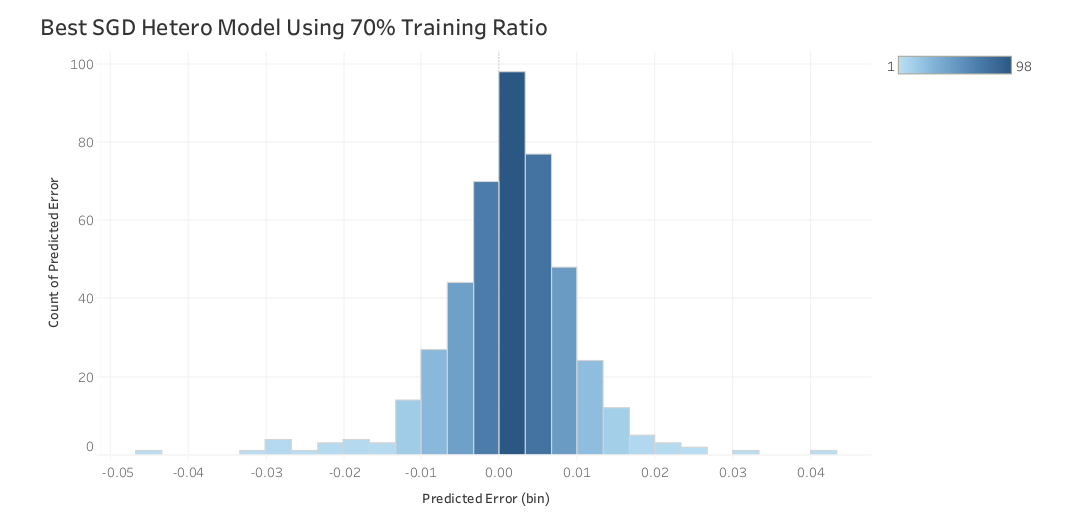
\includegraphics[width=1\textwidth]{hetero_sgd_70}
			\caption{The error produced by SGD Hetero model  using 70\% training ratio}
		\end{figure}
		\pagebreak
		The majority of errors are range from -0.01 to 0.01. The error, actual and predicted value produced by model are shown in following figure in graphical manner.  
		\begin{figure}[hbt!]\centering
			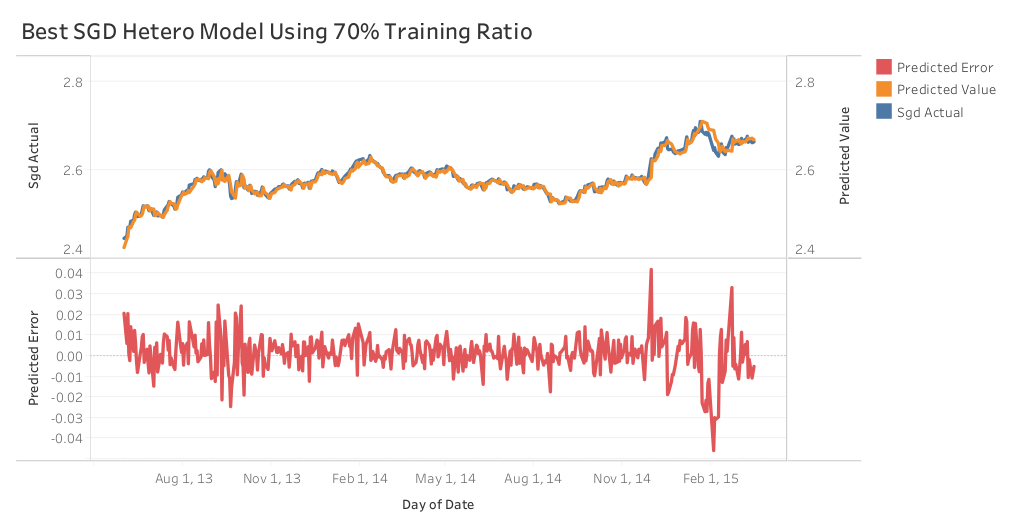
\includegraphics[width=1\textwidth]{best_sgd_hetero_APV_70}
			\caption{The error, actual and predicted value produced by SGD Hetero model using 70\% training ratio }
		\end{figure}
		\pagebreak
		
% SGD Train 60% 
The model which trained with 60\% of the dataset as training dataset are shown in the following table. Same like the previous ratio, the model is  experimented with 10 predictor orders for the homogeneous model, the optimal model for each predictor order, the number of neurons, RMSE, MAE, activation function and fusion function applied are shown in details. The results of the model which trained with 60\% training dataset ratio is shown in following table.
		\\
		
		\setlength{\tabcolsep}{0.5em} % for the horizontal padding
		{\renewcommand{\arraystretch}{1.2}
			
			\begin{table}[ht]
				\centering
				\begin{tabular}{@{}rrrrrrrr@{}}
					\toprule
					\textbf{PO}&\textbf{Neurons}& \textbf{RMSE} & \textbf{MAE} & \textbf{Act\_F}  & \textbf{Learn\_Rate} &\textbf{ Fus\_Fuc}\\ 
					\midrule
					 3 & 5 & 0.006692 & 0.004687 & tanh & 0.1 & MAX \\ 
					 4 & 7 & 0.007332 & 0.005052 & tanh & 0.1 & MAX \\ 
					 5 & 10 & 0.008026 & 0.005470 & tanh & 0.1 & MAX \\ 
					 6 & 15 & 0.007911 & 0.005577 & tanh & 0.1 & MAX \\ 
					 7& 17 & 0.008210 & 0.005781 & tanh & 0.1 & MAX \\ 
					 8 & 9 & 0.007298 & 0.005282 & tanh & 0.1 & MAX \\ 
					 9 & 6 & 0.006856 & 0.004920 & tanh & 0.1 & MAX \\ 
					 10 & 19 & 0.007111 & 0.005144 & tanh & 0.1 & MAX \\
					\hline
				\end{tabular}
				\hspace*{1cm}
				\caption{Results On SGD Heterogeneous Model Using 60\% Training Ratio}
			\end{table}
			
For the 60\% training datasets applied model, the best optimal model produced 0.006692 RMSE value.  This model is obtained with the predictor order 3 with 5 neurons in the hidden layer with the MAX fusion function. The applied activation function hyperbolic tangent function with the learning rate of 0.1.
			
The histogram below explains the minimum and maximum error produced by the best optimal model. The bandwidth of the histogram is 0.00281.
			
			\begin{figure}[hbt!]\centering
				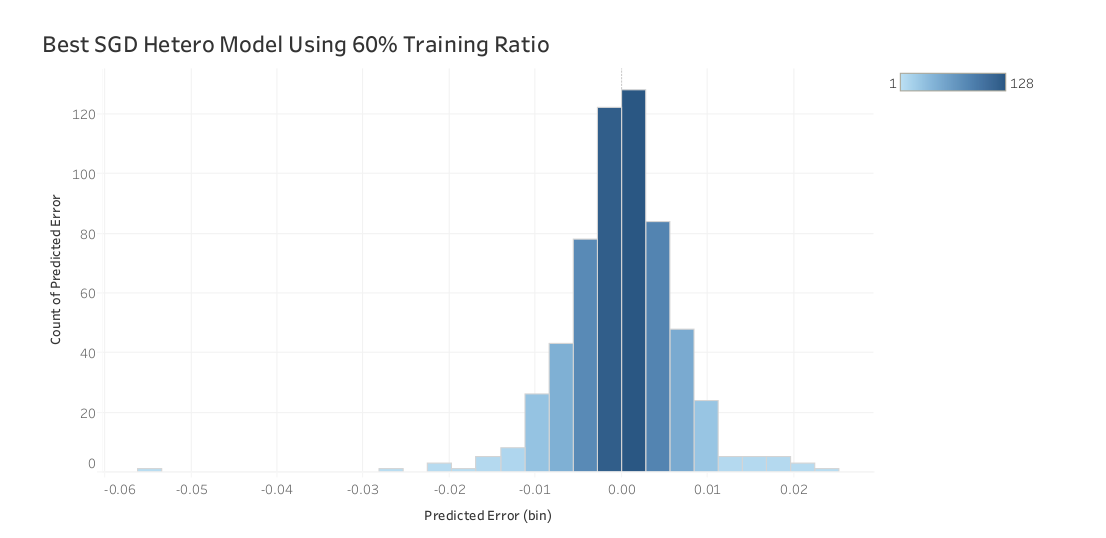
\includegraphics[width=1\textwidth]{hetero_sgd_60}
				\caption{The error produced by SGD Hetero model using 60\% training}
			\end{figure}
			\pagebreak
			
The most errors are lied between -0.01 and 0.01. The following figure compared the actual and predicted values in a line graph manner to demonstrate the difference.
			
			\begin{figure}[hbt!]\centering
				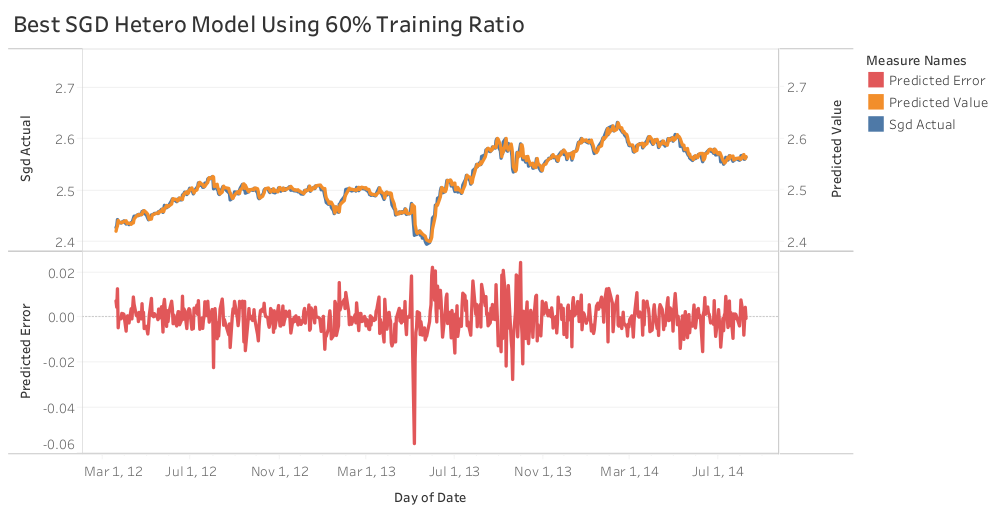
\includegraphics[width=1\textwidth]{best_sgd_hetero_APV_60}
				\caption{The error, actual and predicted value produced by SGD Hetero model using 60\% training ratio}
			\end{figure}
			
The table below summarized the outcomes for three training ratio and their best performance of the homogeneous model for EUR currency.
			
			\setlength{\tabcolsep}{0.5em} % for the horizontal padding
			{\renewcommand{\arraystretch}{1.2}
				
				\begin{table}[ht]
					\centering
					\begin{tabular}{@{}rrrrrrrrr@{}}
						\toprule
						\textbf{Ratio}&\textbf{PO}&\textbf{Neurons}& \textbf{RMSE} & \textbf{MAE} & \textbf{Act\_F} & \textbf{Learn\_Rate} &\textbf{ Fus\_Fuc}\\ 
						\midrule
						60\% & 3 & 5 & 0.006692 & 0.004687 & tanh & 0.1 & MAX \\ 
						70\% & 5 & 5 & 0.008279 & 0.006066 & tanh & 0.1 & MAX \\ 
						80\% & 5 & 6 & 0.013063 & 0.009322 & tanh & 0.1 & MAX \\ 
						\hline
					\end{tabular}
					\hspace*{1cm}
					\caption{The three optimal SGD Hetero models with different training ratio}
					
				\end{table}
Among these heterogeneous models, the model which trained with 60\% ratio is the best model which yield the lowest RMSE error rate. The second best optimal model produced is the model which trained with 70\% training datasets ratio. The 80\% training datasets ratio yield the higher RMSE error than compared to other two. Therefore, this 60\% training ratio produced the best reliable accuracy rate compared to both  80\% training ratio  and 70\% training ratio models.
\subsubsection{Ensemble and Single Models}

The optimal two ensemble models for the SGD to RM exchange rate are shown together with the training ratio that yield the optimal models and their predictor order, RMSE, MAE, activation function, learning rate, and fusion function applied.

\begin{table}[ht]
	\centering
	\begin{tabular}{@{}rrrrrrrrrr@{}}
		\toprule
		\textbf{Ensemble} &\textbf{Ratio}&\textbf{PO}&\textbf{Neurons}& \textbf{RMSE} & \textbf{MAE} & \textbf{Act\_F} & \textbf{LR} &\textbf{ Fus\_Fuc}\\ 
		\midrule
			HOMO	& 60\% & 3 & 5 & 0.006562 & 0.004605 & tanh & 0.1 & MAX \\
			HETERO	& 60\% & 3 & 5 & 0.006692 & 0.004687 & tanh & 0.1 & MAX \\ 
			
			\hline
		\end{tabular}
		\hspace*{1cm}
		\caption{The optimal ensemble  Homo and Hetero models for SGD to RM }
\end{table}

Based on the RMSE rate, the homogeneous ensemble model out perform the heterogeneous model. However, the performance accuracy different for both models is not much, and they both yield better accuracy that current literature accuracy rate for the SGD to RM exchange.

The three  single models for the SGD to RM exchange rate are shown together with the training ratio that yield the optimal models and their predictor order, RMSE, MAE, activation function, and learning rate. Since the homogeneous ensemble yield higher performance accuracy rate, the training parameters from homogeneous model is applied to test in the single models.

\begin{table}[ht]
	\centering
	\begin{tabular}{@{}rrrrrrrrrr@{}}
		\toprule
		\textbf{Single} &\textbf{Ratio}&\textbf{PO}&\textbf{Neurons}& \textbf{RMSE} & \textbf{MAE} & \textbf{Act\_Func} & \textbf{Learn\_Rate} \\ 
		\midrule
		MLP	& 60\% & 3 & 5 & 0.006596 & 0.004628 & tanh & 0.1 \\	
		RNN	& 60\% & 3 & 5 & 0.034397 & 0.028842 & tanh & 0.1 \\
		RBF	& 60\% & 3 & 5 & 0.043879 & 0.040975 & tanh & 0.1  \\
		\hline
	\end{tabular}
	\hspace*{1cm}
	\caption{The optimal three single models for SGD to RM }
\end{table}

Among these single network models, only MLP yield the reliable accuracy compared to ensemble networks models. Therefore, the homogeneous ensemble model produce the best optimal accuracy among both ensemble and single models.

\subsection{AUD to RM}
AUD currency exchange rates data is given as inputs to train with homogeneous, and heterogeneous ensemble models using three different training datasets ratio such as 80\%, 70\%, and 60\%. 

\subsubsection{Homogeneous Model}

The results of the model which applied with 80\% of the dataset as training dataset are shown in the table. 

% AUD Train 80%
\setlength{\tabcolsep}{0.5em} % for the horizontal padding
{\renewcommand{\arraystretch}{1.2}
	\begin{table}[ht]
		
		\begin{tabular}{@{}rrrrrrr@{}}
			\toprule
			\textbf{PO}&\textbf{Neurons}& \textbf{RMSE} & \textbf{MAE} & \textbf{Act\_F}  & \textbf{Learn\_Rate} &\textbf{ Fus\_Fuc}\\ 
			\midrule
			 3 & 6 & 0.019359 & 0.014763 & tanh & 0.1 & MIN \\ 
			 4 & 6 & 0.019278 & 0.014658 & tanh & 0.1 & MAX \\ 
			 5 & 4 & 0.019243 & 0.014585 & logistic & 0.1 & MAX \\ 
			 6 & 5 & 0.019320 & 0.014659 & tanh & 0.1 & MEAN \\ 
			 7 & 18 & 0.019432 & 0.014741 & tanh & 0.1 & MAX \\ 
			 8 & 15 & 0.019457 & 0.014790 & tanh & 0.1 & MAX \\ 
			 9 & 17 & 0.019448 & 0.014756 & tanh & 0.1 & MEAN \\ 
			 10 & 11 & 0.019429 & 0.014681 & tanh & 0.1 & MAX \\ 
			
			\hline
		\end{tabular}
		\hspace*{1cm}
		\caption{Results On AUD Homogeneous Model Using 80\% Training Ratio }
	\end{table}	
	\pagebreak
	
For the 80\% training ratio, the best optimal model  produced 0.019243 RMSE value. The best optimal model which has lowest RMSE error is the predictor order 5 with 4 neurons in the hidden layer with the MAX fusion function. The applied activation function is  logistic sigmoid function with the learning rate of 0.1.
	
The following histogram explain the minimum and maximum error produced by the best optimal model. The bins of the histogram is 0.0256. The bins is based on the range of error values occurred in each model.
	
	\begin{figure}[hbt!]\centering
		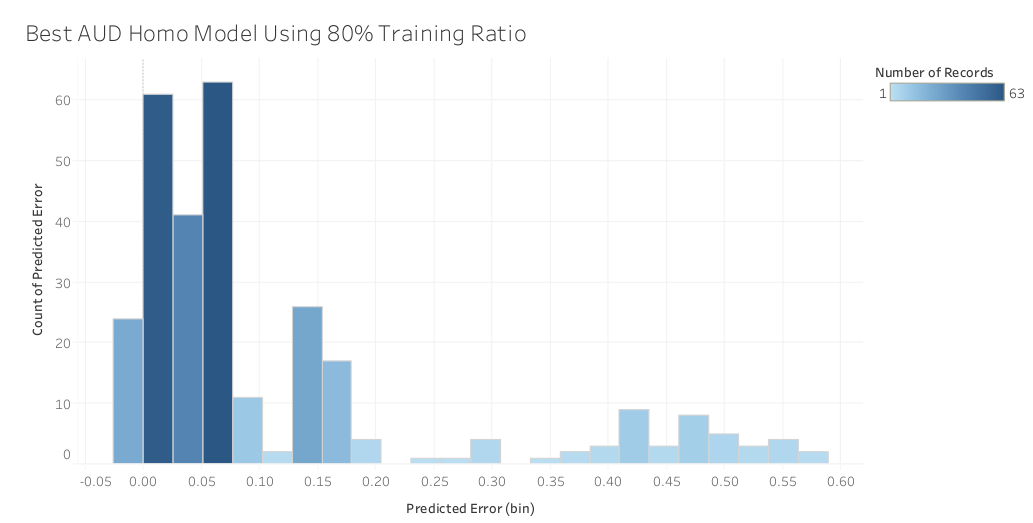
\includegraphics[width=1\textwidth]{homo_aud_80}
		\caption{The error produced by AUD Homo model using 80\% training ratio}
	\end{figure}

The testing dataset, 10\% of the datasets, has 295 testing results, therefore 295 errors are produced. Among these errors results, the majority of the errors are in between -0.05 and 0.02. There are some outliers with the values between 0.40 and 0.60 The error, actual and predicted value produced by model are shown in graphical manner. The following figure   compared the actual and predicted values in a line graph manner to demonstrate the difference along side with error.
	
\begin{figure}[hbt!]\centering
		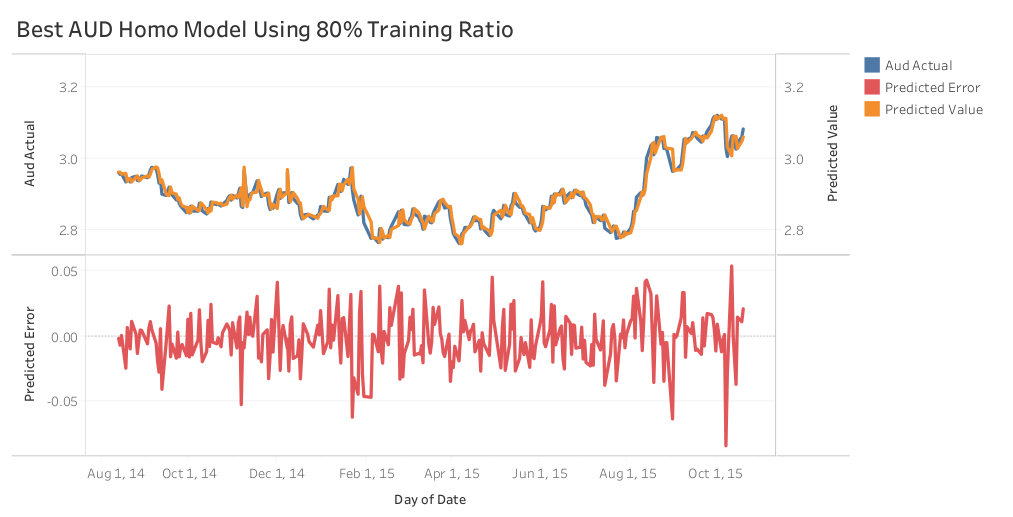
\includegraphics[width=1\textwidth]{best_aud_homo_APV_80}
		\caption{The error, actual and predicted produced by AUD Homo model  value using 80\% training ratio }
	\end{figure}

% AUD Train 70% 
		
The model which trained with 70\% of the dataset as training dataset are shown in table.
	
\pagebreak 	
	\setlength{\tabcolsep}{0.5em} % for the horizontal padding
	{\renewcommand{\arraystretch}{1.2}
		
		\begin{table}[ht]
			\centering
			\begin{tabular}{@{}rrrrrrrr@{}}
				\toprule
				\textbf{PO}&\textbf{Neurons}& \textbf{RMSE} & \textbf{MAE} & \textbf{Act\_F}  & \textbf{Learn\_Rate} &\textbf{ Fus\_Fuc}\\ 
				\midrule
				
				 3 & 6 & 0.016967 & 0.012686 & tanh & 0.1 & MIN \\ 
				 4 & 3 & 0.016945 & 0.012745 & logistic & 0.1 & MIN \\ 
				 5 & 4 & 0.017061 & 0.012822 & logistic & 0.1 & MIN \\ 
				 6 & 7 & 0.017039 & 0.012788 & tanh & 0.1 & MIN \\ 
				 7 & 9 & 0.017000 & 0.012702 & tanh & 0.1 & MIN \\ 
				 8 & 8 & 0.017011 & 0.012716 & tanh & 0.1 & MIN \\ 
				 9 & 5 & 0.017006 & 0.012705 & tanh & 0.1 & MIN \\ 
				 10 & 7 & 0.017078 & 0.012815 & tanh & 0.1 & MIN \\ 
				
				\hline 
				
			\end{tabular}
			\hspace*{1cm}
			\caption{Results On AUD Homogeneous Model Using 70\% Training Ratio }
		\end{table}
		
For the model trained with 70\%, the best optimal model produced 0.016945 RMSE value. The best optimal model which has lowest RMSE error is the predictor order 4 with 3 neurons in the hidden layer with the MIN fusion function. The applied activation function logistic sigmoid function with the learning rate of 0.1.
		
The histogram below explains the minimum and maximum error produced by the best optimal model. The bandwidth of the histogram is 0.0052.
		
		\begin{figure}[hbt!]\centering
			\includegraphics[width=1\textwidth]{homo_aud_70}
			\caption{The error produced by AUD Homogeneous model  using 70\% training ratio}
		\end{figure}
		\pagebreak
		
The testing dataset, 20\% of the datasets, has 443 experiments, which means 443 errors are yield. The majority of errors are range from 0 to 0.07. 
		
		\begin{figure}[hbt!]\centering
			\includegraphics[width=1\textwidth]{best_aud_homo_APV_70}
			\caption{The error, actual and predicted value produced by AUD Homo model using 70\% training ratio }
		\end{figure}
		
		
The error, actual and predicted value produced by model are in graphical manner.  It can said that the error rate is increased in  August 2013, as well as in the early 2015. The model from 70\% training ratio yield better than the model from 80\% training ratio.
		
% AUD Train 60% 
The performance of the model which trained with 60\% of the dataset as training dataset are shown in the following table. 

\setlength{\tabcolsep}{0.5em} % for the horizontal padding
		{\renewcommand{\arraystretch}{1.2}
			\begin{table}[ht]
				\centering
				\begin{tabular}{@{}rrrrrrrr@{}}
					\toprule
					\textbf{PO}&\textbf{Neurons}& \textbf{RMSE} & \textbf{MAE} & \textbf{Act\_F}  & \textbf{Learn\_Rate}&\textbf{ Fus\_Fuc}\\ 
					\midrule
				 3 & 16 & 0.015114 & 0.011438 & tanh & 0.1 & MIN \\ 
				 40 & 7 & 0.015101 & 0.011379 & tanh & 0.1 & MIN \\ 
				 5 & 9 & 0.015139 & 0.011413 & tanh & 0.1 & MIN \\ 
				 6 & 6 & 0.015110 & 0.011385 & tanh & 0.1 & MEAN \\ 
				 7 & 5 & 0.015098 & 0.011373 & tanh & 0.1 & MEAN \\ 
				 8 & 13 & 0.015062 & 0.011370 & tanh & 0.1 & MIN \\ 
				 9 & 5 & 0.015048 & 0.011326 & tanh & 0.1 & MEAN \\ 
				 10 & 15 & 0.015134 & 0.011443 & tanh & 0.1 & MIN \\  
					
					\hline
				\end{tabular}
				\hspace*{1cm}
				\caption{Results On AUD Homogeneous Model Using 60\% Training Ratio}
			\end{table}
			
For the 60\% training datasets applied model, the best optimal model produced 0.015048 RMSE value. The result yield highest  accuracy performance  compared to both the previous models and the current literature result. This model is obtained with the predictor order 9 with 5 neurons in the hidden layer with the MEAN fusion function. The applied activation function hyperbolic tangent function with the learning rate of 0.1.
			
The histogram below explains the minimum and maximum error produced by the best optimal model. The bandwidth of the histogram is 0.0046.
			
			\begin{figure}[hbt!]\centering
				\includegraphics[width=1\textwidth]{homo_aud_60}
				\caption{The error produced by AUD Homo model using 60\%
					training}
			\end{figure}
			
The testing dataset, 20\% of the datasets, has 591 experiments. The most errors are lied between -0.02 and 0.02. The figure below compared the actual and predicted values in a line graph manner to demonstrate the difference.\\
			
\begin{figure}[hbt!]\centering
				\includegraphics[width=1\textwidth]{best_aud_homo_APV_60}
				\caption{The error, actual and predicted value produced by AUD Homo model using 60\% training ratio}
\end{figure}
			\pagebreak
			
			
The Table 6.20 summarized the outcomes for three training ratio and their best performance of the homogeneous model for AUD currency.
			
			\setlength{\tabcolsep}{0.5em} % for the horizontal padding
			{\renewcommand{\arraystretch}{1.2}
				
				\begin{table}[ht]
					\centering
					\begin{tabular}{@{}rrrrrrrrr@{}}
						\toprule
						\textbf{Ratio}&\textbf{PO}&\textbf{Neurons}& \textbf{RMSE} & \textbf{MAE} & \textbf{Act\_F} & \textbf{Learn\_Rate} &\textbf{ Fus\_Fuc}\\ 
						\midrule
						60\% & 9 & 5 & 0.015048 & 0.011326 & tanh & 0.1 & MEAN \\ 
						70\% & 4 & 3 & 0.016945 & 0.012745 & logistic & 0.1 & MIN \\
						80\% & 5 & 4 & 0.019243 & 0.014585 & logistic & 0.1 & MAX \\ 
						\hline
					\end{tabular}
					\hspace*{1cm}
					\caption{The three optimal AUD Homo models with different training ratio}
					
				\end{table}
				
Among these homogeneous models, the model which trained with 60\% ratio is the best model which yield the lowest RMSE error rate. The second best optimal model produced is the model which trained with 70\% training datasets ratio. The 80\% training datasets ratio yield the higher RMSE error than compared to other two. Therefore, this 60\% training ratio produced the best reliable accuracy rate compared to both  80\% training ratio  and 70\% training ratio models.

\subsubsection{Heterogeneous Model}

The results of the model which applied to heterogeneous model with 80\% of the dataset as training dataset are shown in table

% AUD Train 80%
\setlength{\tabcolsep}{0.5em} % for the horizontal padding
{\renewcommand{\arraystretch}{1.2}
	\begin{table}[ht]
		
		\begin{tabular}{@{}rrrrrrr@{}}
			\toprule
			\textbf{PO}&\textbf{Neurons}& \textbf{RMSE} & \textbf{MAE} & \textbf{Act\_F} & \textbf{Learn\_Rate}&\textbf{ Fus\_Fuc} \\ 
			\midrule
			 3 & 3 & 0.019965 & 0.015367 & logistic & 0.1 & MIN \\ 
			 4 & 3 & 0.021491 & 0.016074 & logistic & 0.1 & MIN \\ 
			 5 & 11 & 0.020608 & 0.015830 & logistic & 0.1 & MIN \\ 
			 6 & 12 & 0.021469 & 0.016618 & logistic & 0.1 & MEAN \\ 
			 7 & 10 & 0.019542 & 0.014868 & tanh & 0.1 & MAX \\ 
			 8 & 10 & 0.019607 & 0.014840 & tanh & 0.1 & MAX \\ 
			 9 & 16 & 0.019546 & 0.014922 & tanh & 0.1 & MAX \\ 
			 10 & 18 & 0.019492 & 0.014970 & logistic & 0.1 & MIN \\
			\hline
		\end{tabular}
		\hspace*{1cm}
		\caption{Results On AUD Heterogeneous Model Using 80\% Training Ratio }
	\end{table}	
	
For the 80\% training ratio, the best optimal model  produced 0.019492 RMSE value. The best optimal model which has lowest RMSE error is the predictor order 10 with 18 neurons in the hidden layer with the MIN fusion function. The applied activation function is logistic function with the learning rate of 0.1.
	
The following histogram explain the minimum and maximum error produced by the best optimal model. The bins of the histogram is 0.0256. The bins is based on the range of error values occurred in each model.
	
	\begin{figure}[hbt!]\centering
		\includegraphics[width=1\textwidth]{hetro_aud_80}
		\caption{The error produced by AUD Hetro model using 80\% training ratio}
	\end{figure}
	
	
	The majority of the errors are in between -0.05 and 0.05. The error, actual and predicted value produced by model are shown  in graphical manner. The following figure compared the actual and predicted values in a line graph manner to demonstrate the difference along side with error.
	
	
	\begin{figure}[hbt!]\centering
		\includegraphics[width=0.9\textwidth]{best_aud_hetero_APV_80}
		\caption{The error, actual and predicted produced by AUD Hetero model  value using 80\% training ratio }
	\end{figure}
	\pagebreak
	
% AUD Train 70%
	
The model which trained with 70\% of the dataset as training dataset are shown in table. Same like the previous ratio, the model is  experimented with 10 predictor orders for the homogeneous model, the optimal model for each predictor order, the number of neurons, RMSE, MAE, activation function and fusion function applied are shown in details.
	
The results of the model which trained with 70\% training dataset ratio is shown in following table.
	
	\setlength{\tabcolsep}{0.5em} % for the horizontal padding
	{\renewcommand{\arraystretch}{1.2}
		
		\begin{table}[ht]
			\centering
			\begin{tabular}{@{}rrrrrrrr@{}}
				\toprule
				\textbf{PO}&\textbf{Neurons}& \textbf{RMSE} & \textbf{MAE} & \textbf{Act\_F}  & \textbf{Learn\_Rate} &\textbf{ Fus\_Fuc}\\ 
				\midrule
				 3 & 16 & 0.017101 & 0.012793 & tanh & 0.1 & MAX \\ 
				 4 & 6 & 0.018133 & 0.013553 & logistic & 0.1 & MEAN \\ 
				 5 & 9 & 0.017143 & 0.012856 & tanh & 0.1 & MAX \\ 
				 6 & 10 & 0.017079 & 0.012767 & tanh & 0.1 & MIN \\ 
				 7 & 13 & 0.017648 & 0.013336 & logistic & 0.1 & MIN \\ 
				 8 & 16 & 0.018060 & 0.013493 & logistic & 0.1 & MEAN \\ 
				 9 & 8 & 0.017133 & 0.012797 & logistic & 0.1 & MIN \\ 
				 10 & 15 & 0.017363 & 0.013115 & logistic & 0.1 & MIN \\ 
				\hline
			\end{tabular}
			\hspace*{1cm}
			\caption{Results On AUD Heterogeneous Model Using 70\% Training Ratio }
		\end{table}
		
		For the model trained with 70\%,  the best optimal model produced 0.017079 RMSE value. The best optimal model which has lowest RMSE error is the predictor order 6 with 10 neurons in the hidden layer with the MIN fusion function. The applied activation function hyperbolic tangent function with the learning rate of 0.1.
		
		The histogram below explains the minimum and maximum error produced by the best optimal model. The bandwidth of the histogram is 0.006.
		
		\begin{figure}[hbt!]\centering
			\includegraphics[width=1\textwidth]{hetero_aud_70}
			\caption{The error produced by AUD Hetero model  using 70\% training ratio}
		\end{figure}
		\pagebreak
The majority of errors are range from 0.02 to 0.04. The error, actual and predicted value produced by model are shown in following figure in graphical manner.  
		\begin{figure}[hbt!]\centering
			\includegraphics[width=1\textwidth]{best_aud_hetero_APV_70}
			\caption{The error, actual and predicted value produced by AUD Hetero model using 70\% training ratio }
		\end{figure}
		
		
% AUD Train 60% 
The model which trained with 60\% of the dataset as training dataset are shown in the following table. Same like the previous ratio, the model is  experimented with 10 predictor orders for the homogeneous model, the optimal model for each predictor order, the number of neurons, RMSE, MAE, activation function and fusion function applied are shown in details. The results of the model which trained with 60\% training dataset ratio is shown in following table.
		\\
		
		\setlength{\tabcolsep}{0.5em} % for the horizontal padding
		{\renewcommand{\arraystretch}{1.2}
			
			\begin{table}[ht]
				\centering
				\begin{tabular}{@{}rrrrrrrr@{}}
					\toprule
					\textbf{PO}&\textbf{Neurons}& \textbf{RMSE} & \textbf{MAE} & \textbf{Act\_F}  & \textbf{Learn\_Rate} &\textbf{ Fus\_Fuc}\\ 
					\midrule
					 3 & 17 & 0.015111 & 0.011378 & tanh & 0.1 & MAX \\ 
					 4 & 4 & 0.015166 & 0.011384 & tanh & 0.1 & MAX \\ 
					 5 & 17 & 0.015285 & 0.011529 & tanh & 0.1 & MAX \\ 
					 6 & 4 & 0.015164 & 0.011430 & tanh & 0.1 & MAX \\ 
					 7 & 12 & 0.015187 & 0.011479 & tanh & 0.1 & MAX \\ 
					 8 & 9 & 0.015056 & 0.011347 & tanh & 0.1 & MAX \\ 
					 9 & 8 & 0.015387 & 0.011584 & tanh & 0.1 & MIN \\ 
					 10 & 10 & 0.015308 & 0.011547 & tanh & 0.1 & MAX \\
					\hline
				\end{tabular}
				\hspace*{1cm}
				\caption{Results On AUD Heterogeneous Model Using 60\% Training Ratio}
			\end{table}
			\pagebreak
			
For the 60\% training datasets applied model, the best optimal model produced 0.015111 RMSE value.  This model is obtained with the predictor order 3 with 17 neurons in the hidden layer with the MAX fusion function. The applied activation function hyperbolic tangent function with the learning rate of 0.1.
			
The histogram below explains the minimum and maximum error produced by the best optimal model. The bandwidth of the histogram is 0.0052.
			
			\begin{figure}[hbt!]\centering
				\includegraphics[width=1\textwidth]{hetero_aud_60}
				\caption{The error produced by AUD Hetero model using 60\% training}
			\end{figure}
			\pagebreak
The most errors are lied between -0.02 and 0.02. The following figure compared the actual and predicted values in a line graph manner to demonstrate the difference.
			
			\begin{figure}[hbt!]\centering
				\includegraphics[width=1\textwidth]{best_aud_hetero_APV_60}
				\caption{The error, actual and predicted value produced by AUD Hetero model using 60\% training ratio}
			\end{figure}
			
			The table below summarized the outcomes for three training ratio and their best performance of the homogeneous model for EUR currency.
			
			\setlength{\tabcolsep}{0.5em} % for the horizontal padding
			{\renewcommand{\arraystretch}{1.2}
				
				\begin{table}[ht]
					\centering
					\begin{tabular}{@{}rrrrrrrrr@{}}
						\toprule
						\textbf{Ratio}&\textbf{PO}&\textbf{Neurons}& \textbf{RMSE} & \textbf{MAE} & \textbf{Act\_F} & \textbf{Learn\_Rate} &\textbf{ Fus\_Fuc}\\ 
						\midrule
						60\% & 3 & 17 & 0.015111 & 0.011378 & tanh & 0.1 & MAX \\
						70\% & 6 & 10 & 0.017079 & 0.012767 & tanh & 0.1 & MIN \\ 
						80\% & 10 & 18 & 0.019492 & 0.014970 & logistic & 0.1 & MIN \\
						\hline
					\end{tabular}
					\hspace*{1cm}
					\caption{The three optimal AUD Hetero models with different training ratio}
					
				\end{table}
				Among these heterogeneous models, the model which trained with 60\% ratio is the best model which yield the lowest RMSE error rate. The second best optimal model produced is the model which trained with 70\% training datasets ratio. The 80\% training datasets ratio yield the higher RMSE error than compared to other two. Therefore, this 60\% training ratio produced the best reliable accuracy rate compared to both  80\% training ratio  and 70\% training ratio models.


\subsubsection{Ensemble and Single Models}

The optimal two ensemble models for the AUD to RM exchange rate are shown together with the training ratio that yield the optimal models and their predictor order, RMSE, MAE, activation function, learning rate, and fusion function applied.

\begin{table}[ht]
	\centering
	\begin{tabular}{@{}rrrrrrrrrr@{}}
		\toprule
		\textbf{Ensemble} &\textbf{Ratio}&\textbf{PO}&\textbf{Neurons}& \textbf{RMSE} & \textbf{MAE} & \textbf{Act\_F} & \textbf{LR} &\textbf{ Fus\_Fuc}\\ 
		\midrule
		
		HOMO	& 60\% & 9 & 5 & 0.015048 & 0.011326 & tanh & 0.1 & MEAN \\ 
		HETERO	& 60\% & 3 & 17 & 0.015111 & 0.011378 & tanh & 0.1 & MAX \\
		
		\hline
	\end{tabular}
	\hspace*{1cm}
	\caption{The optimal ensemble  Homo and Hetero models for AUD to RM }
	
\end{table}

Based on the RMSE rate, the homogeneous ensemble model out perform the heterogeneous model. However, the performance accuracy different for both models is not much, and they both yield better accuracy that current literature accuracy rate for the AUD to RM exchange.

The three  single models for the AUD to RM exchange rate are shown together with the training ratio that yield the optimal models and their predictor order, RMSE, MAE, activation function, and learning rate. Since the homogeneous ensemble yield higher performance accuracy rate, the training parameters from homogeneous model is applied to test in the single models.

\begin{table}[ht]
	\centering
	\begin{tabular}{@{}rrrrrrrrrr@{}}
		\toprule
		\textbf{Single} &\textbf{Ratio}&\textbf{PO}&\textbf{Neurons}& \textbf{RMSE} & \textbf{MAE} & \textbf{Act\_Func} & \textbf{Learn\_Rate} \\ 
		\midrule
		MLP	& 60\% & 9 & 5 & 0.015056 & 0.011391 & tanh & 0.1 \\	
		RNN	& 60\% & 9 & 5 & 0.048412 & 0.036032 & tanh & 0.1 \\
		RBF	& 60\% & 9 & 5 & 0.038108 & 0.032192 & tanh & 0.1  \\
		\hline
	\end{tabular}
	\hspace*{1cm}
	\caption{The optimal three single models for AUD to RM }
\end{table}

Among these single network models, only MLP yield the reliable accuracy compared to ensemble networks models. Therefore, the homogeneous ensemble model produce the best optimal accuracy among both ensemble and single models.

	
\subsection{CHF to RM}
CHF currency exchange rates data is given as inputs to train with homogeneous, and heterogeneous ensemble models using three different training datasets ratio such as 80\%, 70\%, and 60\%. 

\subsubsection{Homogeneous Model}

The results of the model which applied with 80\% of the dataset as training dataset are shown in the table. 

% CHF Train 80%
\setlength{\tabcolsep}{0.5em} % for the horizontal padding
{\renewcommand{\arraystretch}{1.2}
	\begin{table}[ht]
		
		\begin{tabular}{@{}rrrrrrr@{}}
			\toprule
			\textbf{PO}&\textbf{Neurons}& \textbf{RMSE} & \textbf{MAE} & \textbf{Act\_F}  & \textbf{Learn\_Rate} &\textbf{ Fus\_Fuc}\\ 
			\midrule
			  3 & 12 & 0.054953 & 0.030650 & tanh & 0.1 & MAX \\ 
			  4 & 20 & 0.050344 & 0.027035 & tanh & 0.1 & MAX \\ 
			  5 & 15 & 0.055322 & 0.030876 & tanh & 0.1 & MAX \\ 
			  6 & 10 & 0.053924 & 0.029521 & tanh & 0.1 & MAX \\ 
			  7 & 4 & 0.059056 & 0.033523 & tanh & 0.1 & MAX \\ 
			  8 & 11 & 0.052332 & 0.028615 & tanh & 0.1 & MAX \\ 
			  9 & 14 & 0.053291 & 0.029243 & tanh & 0.1 & MAX \\ 
			  10 & 16 & 0.054622 & 0.029425 & tanh & 0.1 & MAX \\ 
			\hline
		\end{tabular}
		\hspace*{1cm}
		\caption{Results On CHF Homogeneous Model Using 80\% Training Ratio }
	\end{table}	
	
	
For the 80\% training ratio, the best optimal model  produced 0.050344 RMSE value. The best optimal model which has lowest RMSE error is the predictor order 4 with 20 neurons in the hidden layer with the MAX fusion function. The applied activation function is  hyperbolic tangent function with the learning rate of 0.1.

The following histogram explain the minimum and maximum error produced by the best optimal model. The bins of the histogram is 0.0322. The bins is based on the range of error values occurred in each model.
	
	\begin{figure}[hbt!]\centering
		\includegraphics[width=1\textwidth]{homo_chf_80}
		\caption{The error produced by CHF Homo model using 80\% training ratio}
	\end{figure}
\pagebreak
The testing dataset, 10\% of the datasets, has 295 testing results, therefore 295 errors are produced. Among these errors results, the majority of the errors are in between -0.1 and 0.1. There are some outliers with the values between 0.60 and 0.70 The error, actual and predicted value produced by model are shown in graphical manner.

The following figure   compared the actual and predicted values in a line graph manner to demonstrate the difference along side with error.
	
	\begin{figure}[hbt!]\centering
		\includegraphics[width=1\textwidth]{best_chf_homo_APV_80}
		\caption{The error, actual and predicted produced by CHF Homo model  value using 80\% training ratio }
	\end{figure}
	\pagebreak

% CHF Train 70% 
	
The model which trained with 70\% of the dataset as training dataset are shown in table.
	
	\setlength{\tabcolsep}{0.5em} % for the horizontal padding
	{\renewcommand{\arraystretch}{1.2}
		
		\begin{table}[ht]
			\centering
			\begin{tabular}{@{}rrrrrrrr@{}}
				\toprule
				\textbf{PO}&\textbf{Neurons}& \textbf{RMSE} & \textbf{MAE} & \textbf{Act\_F}  & \textbf{Learn\_Rate} &\textbf{ Fus\_Fuc}\\ 
				\midrule
				
				 3 & 8 & 0.036053 & 0.016791 & tanh & 0.1 & MAX \\ 
				 4 & 19 & 0.035789 & 0.016633 & tanh & 0.1 & MAX \\ 
				 5 & 14 & 0.035763 & 0.016778 & tanh & 0.1 & MAX \\ 
				 6 & 4 & 0.035855 & 0.016864 & tanh & 0.1 & MEAN \\ 
				 7 & 5 & 0.035842 & 0.016704 & logistic & 0.1 & MAX \\ 
				 8 & 20 & 0.035775 & 0.016759 & logistic & 0.1 & MAX \\ 
				 9 & 8 & 0.035708 & 0.016611 & tanh & 0.1 & MAX \\ 
				 10 & 11 & 0.035781 & 0.016691 & logistic & 0.1 & MAX \\ 
				
				\hline 
				
			\end{tabular}
			\hspace*{1cm}
			\caption{Results On CHF Homogeneous Model Using 70\% Training Ratio }
		\end{table}
		
For the model trained with 70\%, the best optimal model produced 0.035708 RMSE value. The best optimal model which has lowest RMSE error is the predictor order 9 with 8 neurons in the hidden layer with the MAX fusion function. The applied activation function hyperbolic tangent function with the learning rate of 0.1.
		
The histogram below explains the minimum and maximum error produced by the best optimal model. The bandwidth of the histogram is 0.0266.
		
		\begin{figure}[hbt!]\centering
			\includegraphics[width=1\textwidth]{homo_chf_70}
			\caption{The error produced by CHF Homogeneous model  using 70\% training ratio}
		\end{figure}
		
		
The testing dataset, 20\% of the datasets, has 443 experiments, which means 443 errors are yield. The majority of errors are range from -0.05 to 0.05. 
		
		\begin{figure}[hbt!]\centering
			\includegraphics[width=1\textwidth]{best_chf_homo_APV_70}
			\caption{The error, actual and predicted value produced by CHF Homo model using 70\% training ratio }
		\end{figure}
		
		
The error, actual and predicted value produced by model are in graphical manner.  It can said that the error rate is increased in the early 2015. The model from 70\% training ratio yield better than the model from 80\% training ratio.
		
% CHF Train 60% 
The performance of the model which trained with 60\% of the dataset as training dataset are shown in the following table. 
		
		\setlength{\tabcolsep}{0.5em} % for the horizontal padding
		{\renewcommand{\arraystretch}{1.2}
			\begin{table}[ht]
				\centering
				\begin{tabular}{@{}rrrrrrrr@{}}
					\toprule
					\textbf{PO}&\textbf{Neurons}& \textbf{RMSE} & \textbf{MAE} & \textbf{Act\_F}  & \textbf{Learn\_Rate}&\textbf{ Fus\_Fuc}\\ 
					\midrule
					 3 & 7 & 0.017547 & 0.013010 & logistic & 0.1 & MEAN \\ 
					 4 & 19 & 0.017559 & 0.013037 & tanh & 0.1 & MAX \\ 
					 5 & 4 & 0.017596 & 0.013092 & tanh & 0.1 & MAX \\ 
					 6 & 4 & 0.017622 & 0.013075 & tanh & 0.1 & MEAN \\ 
					 7 & 7 & 0.017585 & 0.012997 & logistic & 0.1 & MEAN \\ 
					 8 & 7 & 0.017538 & 0.012994 & logistic & 0.1 & MEAN \\ 
					 9 & 6 & 0.017436 & 0.012879 & logistic & 0.1 & MEAN \\ 
					 10 & 15 & 0.017530 & 0.013087 & tanh & 0.1 & MAX \\ 
					\hline
				\end{tabular}
				\hspace*{1cm}
				\caption{Results On CHF Homogeneous Model Using 60\% Training Ratio}
			\end{table}
			
For the 60\% training datasets applied model, the best optimal model produced 0.017436 RMSE value. The result yield highest  accuracy performance  compared to both the previous models and the current literature result. This model is obtained with the predictor order 9 with 6 neurons in the hidden layer with the MEAN fusion function. The applied activation function logistic sigmoid function with the learning rate of 0.1.
			
he histogram below explains the minimum and maximum error produced by the best optimal model. The bandwidth of the histogram is 0.0055.
			
			\begin{figure}[hbt!]\centering
				\includegraphics[width=1\textwidth]{homo_chf_60}
				\caption{The error produced by CHF Homo model using 60\%
					training}
			\end{figure}
			\pagebreak
			
The testing dataset, 20\% of the datasets, has 591 experiments. The most errors are lied between -0.04 and 0.04. The figure below compared the actual and predicted values in a line graph manner to demonstrate the difference.\\
			
			
			
\begin{figure}[hbt!]\centering
				\includegraphics[width=1\textwidth]{best_chf_homo_APV_60}
				\caption{The error, actual and predicted value produced by CHF  Homo model using 60\% training ratio}
\end{figure}

			
			
The Table 6.24 summarized the outcomes for three training ratio and their best performance of the homogeneous model for CHF currency.
			
			\setlength{\tabcolsep}{0.5em} % for the horizontal padding
			{\renewcommand{\arraystretch}{1.2}
				
				\begin{table}[ht]
					\centering
					\begin{tabular}{@{}rrrrrrrrr@{}}
						\toprule
						\textbf{Ratio}&\textbf{PO}&\textbf{Neurons}& \textbf{RMSE} & \textbf{MAE} & \textbf{Act\_F} & \textbf{Learn\_Rate} &\textbf{ Fus\_Fuc}\\ 
						\midrule
						60\% & 9 & 6 & 0.017436 & 0.012879 & logistic & 0.1 & MEAN \\ 
						70\% & 9 & 8 & 0.035708 & 0.016611 & tanh & 0.1 & MAX \\ 
						80\% & 4 & 20 & 0.050344 & 0.027035 & tanh & 0.1 & MAX \\ 
						\hline
					\end{tabular}
					\hspace*{1cm}
					\caption{The three optimal CHF Homo models with different training ratio}
					
				\end{table}
				
Among these homogeneous models, the model which trained with 60\% ratio is the best model which yield the lowest RMSE error rate. The second best optimal model produced is the model which trained with 70\% training datasets ratio. The 80\% training datasets ratio yield the higher RMSE error than compared to other two. Therefore, this 60\% training ratio produced the best reliable accuracy rate compared to both  80\% training ratio  and 70\% training ratio models.
\subsubsection{Heterogeneous Model}


The results of the model which applied to heterogeneous model with 80\% of the dataset as training dataset are shown in table

% CHF Train 80%
\setlength{\tabcolsep}{0.5em} % for the horizontal padding
{\renewcommand{\arraystretch}{1.2}
	\begin{table}[ht]
		
		\begin{tabular}{@{}rrrrrrr@{}}
			\toprule
			\textbf{PO}&\textbf{Neurons}& \textbf{RMSE} & \textbf{MAE} & \textbf{Act\_F} & \textbf{Learn\_Rate}&\textbf{ Fus\_Fuc} \\ 
			\midrule
			 3 & 4 & 0.054999 & 0.033070 & tanh & 0.1 & MAX \\ 
			 4 & 7 & 0.054348 & 0.032888 & tanh & 0.1 & MAX \\ 
			 5 & 6 & 0.055503 & 0.033986 & tanh & 0.1 & MAX \\ 
			 6 & 14 & 0.061526 & 0.037150 & tanh & 0.1 & MAX \\ 
			 7 & 20 & 0.058428 & 0.036019 & logistic & 0.1 & MAX \\ 
			 8 & 12 & 0.060366 & 0.035037 & tanh & 0.1 & MAX \\ 
			 9 & 14 & 0.052859 & 0.030139 & tanh & 0.1 & MAX \\ 
			 10 & 17 & 0.059115 & 0.037108 & logistic & 0.1 & MAX \\ 
			
			\hline
		\end{tabular}
		\hspace*{1cm}
		\caption{Results On CHF Heterogeneous Model Using 80\% Training Ratio }
	\end{table}	
	
	For the 80\% training ratio, the best optimal model  produced 0.052859 RMSE value. The best optimal model which has lowest RMSE error is the predictor order 9 with 14 neurons in the hidden layer with the MAX fusion function. The applied activation function is hyperbolic tangent function with the learning rate of 0.1.
	
	The following histogram explain the minimum and maximum error produced by the best optimal model. The bins of the histogram is 0.015. The bins is based on the range of error values occurred in each model.
	
	\begin{figure}[hbt!]\centering
		\includegraphics[width=1\textwidth]{hetro_chf_80}
		\caption{The error produced by CHF Hetro model using 80\% training ratio}
	\end{figure}
	
	
The majority of the errors are in between -0.06 and 0.04. The error, actual and predicted value produced by model are shown  in graphical manner. The following figure compared the actual and predicted values in a line graph manner to demonstrate the difference along side with error.
	
	
	\begin{figure}[hbt!]\centering
		\includegraphics[width=0.9\textwidth]{best_chf_hetero_APV_80}
		\caption{The error, actual and predicted produced by CHF Hetero model  value using 80\% training ratio }
	\end{figure}
	\pagebreak
	
	% CHF Train 70%
	
The model which trained with 70\% of the dataset as training dataset are shown in table. Same like the previous ratio, the model is  experimented with 10 predictor orders for the homogeneous model, the optimal model for each predictor order, the number of neurons, RMSE, MAE, activation function and fusion function applied are shown in details.
	
	
	The results of the model which trained with 70\% training dataset ratio is shown in following table.
	
	\setlength{\tabcolsep}{0.5em} % for the horizontal padding
	{\renewcommand{\arraystretch}{1.2}
		
		\begin{table}[ht]
			\centering
			\begin{tabular}{@{}rrrrrrrr@{}}
				\toprule
				\textbf{PO}&\textbf{Neurons}& \textbf{RMSE} & \textbf{MAE} & \textbf{Act\_F}  & \textbf{Learn\_Rate} &\textbf{ Fus\_Fuc}\\ 
				\midrule
				 3 & 18 & 0.036308 & 0.016807 & tanh & 0.1 & MAX \\ 
				 4 & 17 & 0.036467 & 0.017211 & tanh & 0.1 & MAX \\ 
				 5 & 15 & 0.035976 & 0.017074 & tanh & 0.1 & MAX \\ 
				 6 & 6 & 0.037078 & 0.017726 & tanh & 0.1 & MAX \\ 
				 7 & 19 & 0.037439 & 0.018094 & tanh & 0.1 & MAX \\ 
				 8 & 5 & 0.040298 & 0.023220 & tanh & 0.1 & MAX \\ 
				 9 & 19 & 0.037304 & 0.018113 & tanh & 0.1 & MAX \\ 
				 10 & 8 & 0.036631 & 0.017312 & tanh & 0.1 & MAX \\ 
				\hline
			\end{tabular}
			\hspace*{1cm}
			\caption{Results On CHF Heterogeneous Model Using 70\% Training Ratio }
		\end{table}
		
		For the model trained with 70\%,  the best optimal model produced 0.035976 RMSE value. The best optimal model which has lowest RMSE error is the predictor order 5 with 15 neurons in the hidden layer with the MAX fusion function. The applied activation function hyperbolic tangent function with the learning rate of 0.1.
		
		The histogram below explains the minimum and maximum error produced by the best optimal model. The bandwidth of the histogram is 0.006.
		
		\begin{figure}[hbt!]\centering
			\includegraphics[width=1\textwidth]{hetero_chf_70}
			\caption{The error produced by CHF Hetero model  using 70\% training ratio}
		\end{figure}
		
		The majority of errors are range from -0.05 to 0.05. The error, actual and predicted value produced by model are shown in following figure in graphical manner.  
		\begin{figure}[hbt!]\centering
			\includegraphics[width=1\textwidth]{best_chf_hetero_APV_70}
			\caption{The error, actual and predicted value produced by CHF Hetero model using 70\% training ratio }
		\end{figure}
		\pagebreak
		
% CHF Train 60% 
The model which trained with 60\% of the dataset as training dataset are shown in the following table. Same like the previous ratio, the model is  experimented with 10 predictor orders for the homogeneous model, the optimal model for each predictor order, the number of neurons, RMSE, MAE, activation function and fusion function applied are shown in details. The results of the model which trained with 60\% training dataset ratio is shown in following table.
		\\
		
		\setlength{\tabcolsep}{0.5em} % for the horizontal padding
		{\renewcommand{\arraystretch}{1.2}
			
			\begin{table}[ht]
				\centering
				\begin{tabular}{@{}rrrrrrrr@{}}
					\toprule
					\textbf{PO}&\textbf{Neurons}& \textbf{RMSE} & \textbf{MAE} & \textbf{Act\_F}  & \textbf{Learn\_Rate} &\textbf{ Fus\_Fuc}\\ 
					\midrule
					 3 & 20 & 0.017658 & 0.013140 & tanh & 0.1 & MAX \\ 
					 4 & 13 & 0.017903 & 0.013263 & tanh & 0.1 & MAX \\ 
					 5 & 11 & 0.017901 & 0.013260 & tanh & 0.1 & MAX \\ 
					 6 & 14 & 0.022585 & 0.016937 & logistic & 0.1 & MEAN \\ 
					 7 & 19 & 0.017690 & 0.013070 & tanh & 0.1 & MAX \\ 
					 8 & 18 & 0.017514 & 0.012996 & tanh & 0.1 & MAX \\ 
					 9 & 14 & 0.019867 & 0.015276 & tanh & 0.1 & MEAN \\ 
					 10 & 15 & 0.017603 & 0.013097 & tanh & 0.1 & MAX \\ 
					\hline
				\end{tabular}
				\hspace*{1cm}
				\caption{Results On CHF Heterogeneous Model Using 60\% Training Ratio}
			\end{table}
			
			For the 60\% training datasets applied model, the best optimal model produced 0.017514 RMSE value.  This model is obtained with the predictor order 8 with 18 neurons in the hidden layer with the MAX fusion function. The applied activation function hyperbolic tangent function with the learning rate of 0.1.
			
			The histogram below explains the minimum and maximum error produced by the best optimal model. The bandwidth of the histogram is 0.0045.
			
			\begin{figure}[hbt!]\centering
				\includegraphics[width=1\textwidth]{hetero_chf_60}
				\caption{The error produced by CHF Hetero model using 60\% training}
			\end{figure}
			
			The most errors are lied between -0.02 and 0.02. The following figure compared the actual and predicted values in a line graph manner to demonstrate the difference.
			
			\begin{figure}[hbt!]\centering
				\includegraphics[width=1\textwidth]{best_chf_hetero_APV_60}
				\caption{The error, actual and predicted value produced by CHF Hetero model using 60\% training ratio}
			\end{figure}
			
			The table below summarized the outcomes for three training ratio and their best performance of the homogeneous model for EUR currency.
			
			\setlength{\tabcolsep}{0.5em} % for the horizontal padding
			{\renewcommand{\arraystretch}{1.2}
				
				\begin{table}[ht]
					\centering
					\begin{tabular}{@{}rrrrrrrrr@{}}
						\toprule
						\textbf{Ratio}&\textbf{PO}&\textbf{Neurons}& \textbf{RMSE} & \textbf{MAE} & \textbf{Act\_F} & \textbf{Learn\_Rate} &\textbf{ Fus\_Fuc}\\ 
						\midrule
						60\% & 8 & 18 & 0.017514 & 0.012996 & tanh & 0.1 & MAX \\  
						70\% & 5 & 15 & 0.035976 & 0.017074 & tanh & 0.1 & MAX \\
						80\% & 9 & 14 & 0.052859 & 0.030139 & tanh & 0.1 & MAX \\
						\hline
					\end{tabular}
					\hspace*{1cm}
					\caption{The three optimal CHF Hetero models with different training ratio}
					
				\end{table}
				\pagebreak
Among these heterogeneous models, the model which trained with 60\% ratio is the best model which yield the lowest RMSE error rate. The second best optimal model produced is the model which trained with 70\% training datasets ratio. The 80\% training datasets ratio yield the higher RMSE error than compared to other two. Therefore, this 60\% training ratio produced the best reliable accuracy rate compared to both  80\% training ratio  and 70\% training ratio models.
\subsubsection{Ensemble and Single Models}

The optimal two ensemble models for the CHF to RM exchange rate are shown together with the training ratio that yield the optimal models and their predictor order, RMSE, MAE, activation function, learning rate, and fusion function applied.

\begin{table}[ht]
	\centering
	\begin{tabular}{@{}rrrrrrrrrr@{}}
		\toprule
		\textbf{Ensemble} &\textbf{Ratio}&\textbf{PO}&\textbf{Neurons}& \textbf{RMSE} & \textbf{MAE} & \textbf{Act\_F} & \textbf{LR} &\textbf{ Fus\_Fuc}\\ 
		\midrule
		
		
		HOMO	& 60\% & 9 & 6 & 0.017436 & 0.012879 & logistic & 0.1 & MEAN \\
		HETERO	& 60\% & 8 & 18 & 0.017514 & 0.012996 & tanh & 0.1 & MAX \\  
		
		\hline
	\end{tabular}
	\hspace*{1cm}
	\caption{The optimal ensemble  Homo and Hetero models for CHF to RM }
	
\end{table}

Based on the RMSE rate, the homogeneous ensemble model out perform the heterogeneous model. However, the performance accuracy different for both models is not much, and they both yield better accuracy that current literature accuracy rate for the CHF to RM exchange.

The three  single models for the CHF to RM exchange rate are shown together with the training ratio that yield the optimal models and their predictor order, RMSE, MAE, activation function, and learning rate. Since the homogeneous ensemble yield higher performance accuracy rate, the training parameters from homogeneous model is applied to test in the single models.

\begin{table}[ht]
	\centering
	\begin{tabular}{@{}rrrrrrrrrr@{}}
		\toprule
		\textbf{Single} &\textbf{Ratio}&\textbf{PO}&\textbf{Neurons}& \textbf{RMSE} & \textbf{MAE} & \textbf{Act\_Func} & \textbf{Learn\_Rate} \\ 
		\midrule
		MLP	& 60\% & 9 & 6 & 0.017722 & 0.013076 & tanh & 0.1 \\	
		RNN	& 60\% & 9 & 6 & 0.031643 & 0.024210 & tanh & 0.1 \\
		RBF	& 60\% & 9 & 6 & 0.039575 & 0.0317153 & tanh & 0.1  \\
		\hline
	\end{tabular}
	\hspace*{1cm}
	\caption{The optimal three single models for CHF to RM }
\end{table}

Among these single network models, only MLP yield the reliable accuracy compared to ensemble networks models. Therefore, the homogeneous ensemble model produce the best optimal accuracy among both ensemble and single models.


\section{Research Findings}	

For all the currencies, the models with trained with 60\% training inputs yield the best accuracy performance for both homogeneous and heterogeneous ensemble models.

The performance comparisons for both ensemble model based on the RMSE performance demonstrated in the following figure.  
\begin{figure}[hbt!]\centering
	\includegraphics[width=1\textwidth]{compare_homo_hetero}
	\caption{Comparison between optimal Ensemble Heterogeneous and Homogeneous Model}
\end{figure}

It can be said that both models yield the similar performance, but homogeneous ensemble model outperformed the heterogeneous model.

While comparing with current literature result, it is found that USD currency performance is better then current result which used MLFN (Multi-layered feed forward network)  \cite{chan:2010}. The comparisons with current literature result is further demonstrated in following table.


\begin{table}[ht]
	\centering
	\begin{tabular}{@{}rrrrrrrrrr@{}}
		\toprule
		\textbf{ANN Models}  & \textbf{RMSE} & \textbf{MAE} \\ 
		\midrule
		Homogeneous	 & 0.012598 & 0.009269 \\	
		Heterogeneous & 0.0.12704 & 0.009321  \\
		MLFN  & 0.02065 & 0.01644 \\
		\hline
	\end{tabular}
	\hspace*{1cm}
	\caption{The performance of Ensemble models compared with literature result for USD currency }
\end{table}

These two ensemble model are compared with the single models performance as well. It is found that the ensemble models outperformed the single models, and the MLP single model yield the best performance for the single models for every currency. The figure 6.74 explained their performance comparison.


\begin{figure}[hbt!]\centering
	\includegraphics[width=1\textwidth]{ensemble_single}
	\caption{Comparison between Ensemble and Single Models Performance}
\end{figure}

\pagebreak





\section{Research Contributions}

From the findings discussed above, the homogeneous model trained with 60\% training ratio produce the best optimal model for the all six currency exchange rate. In the current literature, there is only USD to RM exchange rate forecasting using ANNs methods are found. The project contributed by constructing the ensemble model which yield better performance. Moreover, other currency exchange rate such as GBP, EUR, SGD, AUD, and CHF are also forecasted using the same approach with USD to RM exchange rate forecasting.



\section{Future Work}

This project can be extended by increasing the number of predictor order since the project only experimented with predictor number 3 until 10. Moreover, the influence factors such the economic and political situation of the respective exchange rate should put as training inputs parameters. The methods of constructing the ensemble models can be also altered. 


\section{Conclusion}


The performance of ensemble models, homogeneous and heterogeneous models are compared with the single model, which are MLP, RNN, and RBF. The findings conclude that the homogeneous model trained with 60\% training ratio produce the best optimal model for the all six currency exchange rate. For the USD, the optimal homogeneous  performance is 0.012598 RMSE values. This performance is better than current literature performance. Other exchange rates forecasting is also produced reliable performance.